\chapter{Advanced UAV Control}
\section{Motivation}
\begin{figure}[htbp]
	\centering
	\framebox{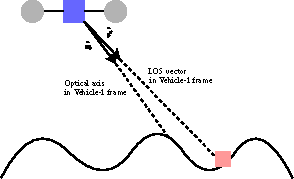
\includegraphics[width=0.6\textwidth]{images/chapter4/advanced_control_motivation.pdf}}
	\caption{Non-flat-earth model example. The unit optical axis vector $\hat{m}$ and the unit line of sight vector $\hat{l}$ are key components of the controller presented in this chapter.}
	\label{nonflatearth}
\end{figure}
The UAV control algorithm introduced in the previous chapter is relatively simple and easy to implement. However, the controller makes strong assumption that can be unrealistic in some cases. For example, it assumes that the line of sight (LOS) vector to the target and the optical axis terminate on the same flat surface which is often called 'flat-earth assumption.' In that case, the altitude of the multirotor acts as a scale factor that can be used to compute how much the UAV should move forward. The more advanced UAV controller presented in this chapter overcomes the flat-earth assumption by working with the unit LOS vector and unit optical axis vector (see Figure \ref{nonflatearth}). Also, the controller does not require the altitude of the multirotor to be known because the scale factor does not have to be recovered.

\section{Controller Derivation for Simple UAV Dynamics}
\begin{figure}[htbp]
	\centering
	\framebox{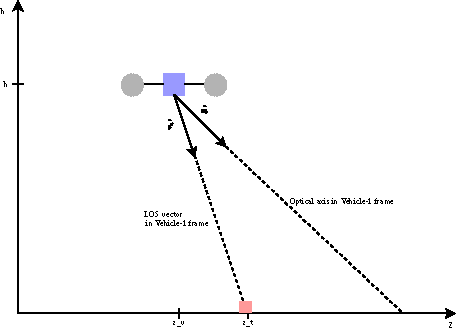
\includegraphics[width=0.6\textwidth]{images/chapter4/advanced_control_overview.pdf}}
	\caption{Graphical overview of the problem}
	\label{overview}
\end{figure}

As a first step in developing the control algorithm, we start with the simple vehicle dynamics  
\begin{equation}
\ddot{z}_v=u_1
\end{equation}
\begin{equation}
\ddot{h}=u_2
\end{equation} 
where $z_v$ is multirotor's horizontal position and $h$ is its altitude.
A required input to the proposed controller is the measured unit LOS vector $\hat{l}$. 
Let $\hat{m}$ be the unit vector aligned with the optical axis, and let the projection matrix onto the null space of $\hat{m}$ be 
\begin{equation}
P_{\hat{m}}=(I-\hat{m}\hat{m}^\top).
\end{equation}
Selecting the coordinate frame as $(\hat{z},\ \hat{z}\times\hat{h},\ \hat{h})$, $\hat{m}$ can be represented as 
\begin{equation}
\hat{m}=\begin{pmatrix}
m_1 & 0 & -m_2
\end{pmatrix}^\top.
\end{equation}
In that case, we have 
\begin{align}
P_{\hat{m}}&=\begin{pmatrix}1 & 0 & 0 \\ 0 & 1 & 0 \\ 0 & 0 & 1 \end{pmatrix}
-\begin{pmatrix} m_1 \\ 0 \\ -m_2 \end{pmatrix}\begin{pmatrix} m_1 & 0 & -m_2 \end{pmatrix}
\\&=\begin{pmatrix}1-m_1^2 & 0 & m_1m_2 \\ 0 & 1 & 0 \\ m_1m_2 & 0 & 1-m_2^2 \end{pmatrix}.
\label{p_mhat}
\end{align}
Note that the controller is developed as if the multirotor is in 3D plane even if we only show 2D dynamics.
\begin{figure}[htbp]
	\centering
	\framebox{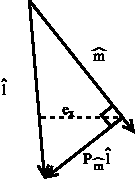
\includegraphics[width=0.2\textwidth]{images/chapter4/projection.pdf}}
	\caption{Projection onto the null space of the optical axis unit vector}
	\label{projection}
\end{figure}
The objective is to drive the horizontal component of $P_{\hat{m}}\hat{l}$ to zero. If we let
\begin{equation}
\hat{e}_1=[1 \quad 0 \quad 0]^\top,
\label{e_1}
\end{equation}
the horizontal component of $P_{\hat{m}}\hat{l}$ which is denoted by $e_x$ can be expressed as
\begin{equation}
e_x=\hat{e}_1^{\top}P_{\hat{m}}\hat{l}.
\end{equation}
Note that since $\hat{m}$ is fixed and known and $\hat{l}$ is measured, $e_x$ can also be measured. Also, since $\dot{\hat{l}}$ can be approximated by differentiating numerically,
\begin{equation}
\dot{e}_x=\hat{e}_1^{\top}P_{\hat{m}}\dot{\hat{l}}
\label{exdot}
\end{equation} is measurable.
Meanwhile, the line of sight vector is
\begin{equation}
l=\begin{pmatrix} z_t \\ 0 \\ 0 \end{pmatrix}
-\begin{pmatrix} z_v \\ 0 \\ h \end{pmatrix}.
\label{los}
\end{equation}
Differentiating equation (\ref{los}) gives 
\begin{equation}
\dot{l}=\begin{pmatrix} \dot{z}_t \\ 0 \\ 0 \end{pmatrix}
-\begin{pmatrix} \dot{z}_t \\ 0 \\ \dot{h} \end{pmatrix},
\end{equation}
and
\begin{equation}
\ddot{l}=\begin{pmatrix} \ddot{z}_t \\ 0 \\ 0 \end{pmatrix}
-\begin{pmatrix} \ddot{z}_v \\ 0 \\ \ddot{h} \end{pmatrix}.
\end{equation}
Assuming that the velocity of the target and the UAV altitude (i.e. $u_2=0$) are not changing yields
\begin{equation}
\ddot{l}=\begin{pmatrix} -\ddot{z}_v \\ 0 \\ 0 \end{pmatrix}
=\begin{pmatrix} -u_1 \\ 0 \\ 0 \end{pmatrix}.
\label{lddot}
\end{equation}
Thus, combining equations (\ref{p_mhat}), (\ref{e_1}) and (\ref{lddot})
results in 
\begin{equation}
\hat{e}_1^{\top}P_{\hat{m}}\ddot{l}=-(1-m_1^2)u_1.
\label{eplddot}
\end{equation}
Let
\begin{equation}
L=\norm{l},
\end{equation} be the unknown depth between the camera and the target, or the norm of the LOS vector. Then, the unit LOS vector is 
\begin{equation}
\hat{l}=\frac{l}{L}.
\label{lhat}
\end{equation}
Differentiating equation (\ref{lhat}) gives
\begin{equation}
\dot{\hat{l}}=\frac{\dot{l}L-l\dot{L}}{L^2}=\frac{\dot{l}}{L}-\hat{l}\bigg(\frac{\dot{L}}{L}\bigg).
\label{lhatdot}
\end{equation}
Differentiating again gives
\begin{align}
\ddot{\hat{l}}&=\frac{\ddot{l}L-\dot{l}\dot{L}}{L^2}-\dot{\hat{l}}\bigg(\frac{\dot{L}}{L}\bigg)-\hat{l}\bigg(\frac{\ddot{L}L-\dot{L}^2}{L^2}\bigg)
\\&=\frac{\ddot{l}}{L}-\bigg(\frac{\dot{l}}{L}\bigg)\bigg(\frac{\dot{L}}{L}\bigg)-\dot{\hat{l}}\bigg(\frac{\dot{L}}{L}\bigg)-\hat{l}\bigg(\frac{\ddot{L}}{L}\bigg)+\hat{l}\bigg(\frac{\dot{L}}{L}\bigg)^2.
\label{lhatddot}
\end{align}
Plugging in for $\frac{\dot{l}}{L}=\dot{\hat{l}}+\hat{l}\bigg(\frac{\dot{L}}{L}\bigg)$ from equation (\ref{lhatdot}) gives
\begin{equation}
\ddot{\hat{l}}=\frac{\ddot{l}}{L}-2\dot{\hat{l}}\bigg(\frac{\dot{L}}{L}\bigg)-\hat{l}\bigg(\frac{\ddot{L}}{L}\bigg).
\label{lhatddot}
\end{equation}
Differentiating equation (\ref{exdot}) and using equation (\ref{lhatddot}) for $\ddot{\hat{l}}$ yields
\begin{align}
\ddot{e}_x&=\hat{e}_1^{\top}P_{\hat{m}}\ddot{\hat{l}}
\\&=\hat{e}_1^{\top}P_{\hat{m}}\bigg(\frac{\ddot{l}}{L}-2\dot{\hat{l}}\bigg(\frac{\dot{L}}{L}\bigg)-\hat{l}\bigg(\frac{\ddot{L}}{L}\bigg)\bigg)
\\&=\frac{1}{L}(\hat{e}_1^{\top}P_{\hat{m}}\ddot{l})+\frac{\dot{L}}{L}(-2\hat{e}_1^{\top}P_{\hat{m}}\dot{\hat{l}})+\frac{\ddot{L}}{L}(-\hat{e}_1^{\top}P_{\hat{m}}\hat{l}).
\end{align}
Substituting (\ref{eplddot}) for $\hat{e_1}^{\top}P_{\hat{m}}\ddot{l}$ results in  
\begin{equation}
\ddot{e}_x=-\frac{1}{L}(1-m_1^2)u_1+\frac{\dot{L}}{L}(-2\hat{e}_1^{\top}P_{\hat{m}}\dot{\hat{l}})+\frac{\ddot{L}}{L}(-\hat{e}_1^{\top}P_{\hat{m}}\hat{l}).
\end{equation} 
Defining the unknown quantities
\begin{equation}
\beta_1\triangleq\frac{1}{L},\quad \beta_2\triangleq\frac{\dot{L}}{L}, \quad \beta_3\triangleq\frac{\ddot{L}}{L}
\end{equation}
and the measured quantities
\begin{equation}
\phi_1=1-m_1^2,\quad \phi_2=-2\hat{e}_1^{\top}P_{\hat{m}}\dot{\hat{l}}, \quad \phi_3=-\hat{e}_1^{\top}P_{\hat{m}}\hat{l}.
\end{equation}
we can rewrite 
\begin{equation}
\ddot{e}_x=-\beta_1\phi_1u_1+\beta_2\phi_2+\beta_3\phi_3.
\label{exddot}
\end{equation}

In order to drive $e_x$ to zero, define
\begin{equation}
s=\dot{e}_x+ke_x
\label{s}
\end{equation} where $k>0$. The reason why the equation (\ref{s}) is selected is because when $s\rightarrow0$, 
\begin{equation}
\dot{e}_x=-ke_x
\end{equation} which makes $e_x$ asymptotically stable. Thus, if we can find the control input $u_1$ that makes $s\rightarrow0$, $e_x$ will converge to zero. Differentiating equation (\ref{s}) and substituting (\ref{exddot}) for $\ddot{e}_x$ yields
\begin{align}
\dot{s}&=\ddot{e}_x+k\dot{e}_x
\\&=-\beta_1\phi_1u_1+\beta_2\phi_2+\beta_3\phi_3+k\dot{e}_x.
\label{sdot}
\end{align}
If $\beta_1$, $\beta_2$, and $\beta_3$ are known, then the ideal control input would be 
\begin{equation}
u_1=\frac{1}{\beta_1\phi_1}(\beta_2\phi_2+\beta_3\phi_3+k\dot{e}_x+\alpha s)
\end{equation}
where $\alpha>0$.
Then, 
\begin{equation}
\dot{s}=-\alpha s
\end{equation} 
which makes $s$ asymptotically stable. 
However, since we do not know $\beta_1$, $\beta_2$, and $\beta_3$, we use the control input
\begin{equation}
u_1=\frac{1}{\hat{\beta}_1\phi_1}(\hat{\beta}_2\phi_2+\hat{\beta}_3\phi_3+k\dot{e}_x+\alpha s)
\label{actualcontrol}
\end{equation}
where $\hat{\beta}_1$, $\hat{\beta}_2$, and $\hat{\beta}_3$ are the estimates of $\beta_1$, $\beta_2$, and $\beta_3$ respectively. 
In that case, we have
\begin{align}
\dot{s}&=-\beta_1\phi_1u_1+\hat{\beta}_1\phi_1u_1-\hat{\beta}_1\phi_1u_1+\beta_2\phi_2+\beta_3\phi_3+k\dot{e}_x
\label{sdot1}
\\&=-(\beta_1-\hat{\beta}_1)\phi_1u_1+(\beta_2-\hat{\beta}_2)\phi_2+(\beta_3-\hat{\beta}_3)\phi_3-\alpha s
\\&=-\tilde{\beta}_1\phi_1u_1+\tilde{\beta}_2\phi_2+\tilde{\beta}_3\phi_3-\alpha s
\\&=\tilde{B}^\top\Phi-\alpha s
\label{sdot2}
\end{align}
where 
\begin{equation}
B\triangleq\begin{pmatrix}
\beta_1 \\ \beta_2 \\ \beta_3
\end{pmatrix}, \quad
\hat{B}\triangleq\begin{pmatrix} \hat{\beta}_1 \\ \hat{\beta}_2 \\ \hat{\beta}_3 \end{pmatrix}, \quad
\tilde{B}\triangleq B-\hat{B}, \quad 
\Phi \triangleq \begin{pmatrix} -\phi_1u_1 \\ \phi_2 \\ \phi_3 \end{pmatrix}.
\end{equation}
Selecting the Lyapunov function
\begin{equation}
V=\frac{1}{2}s^2+\frac{1}{2}\tilde{B}^\top \Gamma^{-1}\tilde{B},
\label{v}
\end{equation}
and differentiating with respect to time gives
\begin{align}
\dot{V}&=s\dot{s}+\tilde{B}^\top \Gamma^{-1}\dot{\tilde{B}}
\\&=s(\tilde{B}^\top\Phi-\alpha s)+\tilde{B}^\top \Gamma^{-1}\dot{\tilde{B}}
\\&=-\alpha s^2+\tilde{B}^\top(s\Phi+\Gamma^{-1}\dot{\tilde{B}}).
\label{vdot}
\end{align}
Assuming $B$ is roughly constant or slowly varying (i.e. $\dot{B}=0$), we have that $\dot{\tilde{B}}=-\dot{\hat{B}}$ implying that
\begin{equation}
\dot{V}=-\alpha s^2+\tilde{B}^\top(s\Phi-\Gamma^{-1}\dot{\hat{B}}).
\end{equation}
Therefore, by choosing $\dot{\hat{B}}=s\Gamma\Phi$, gives
\begin{equation}
\dot{V}=-\alpha s^2
\end{equation}
which implies that $s$ is asymptotically stable. Thus, the original objective of stabilizing $e_x$ is achieved. This control scheme is simulated in Simulink and Figures \ref{simple_simulation} and \ref{another_simple_simulation} show the performance of the controller for one initial condition. 
\begin{figure}[htbp]
	\centering
	\begin{subfigure}[t]{0.45\linewidth}
		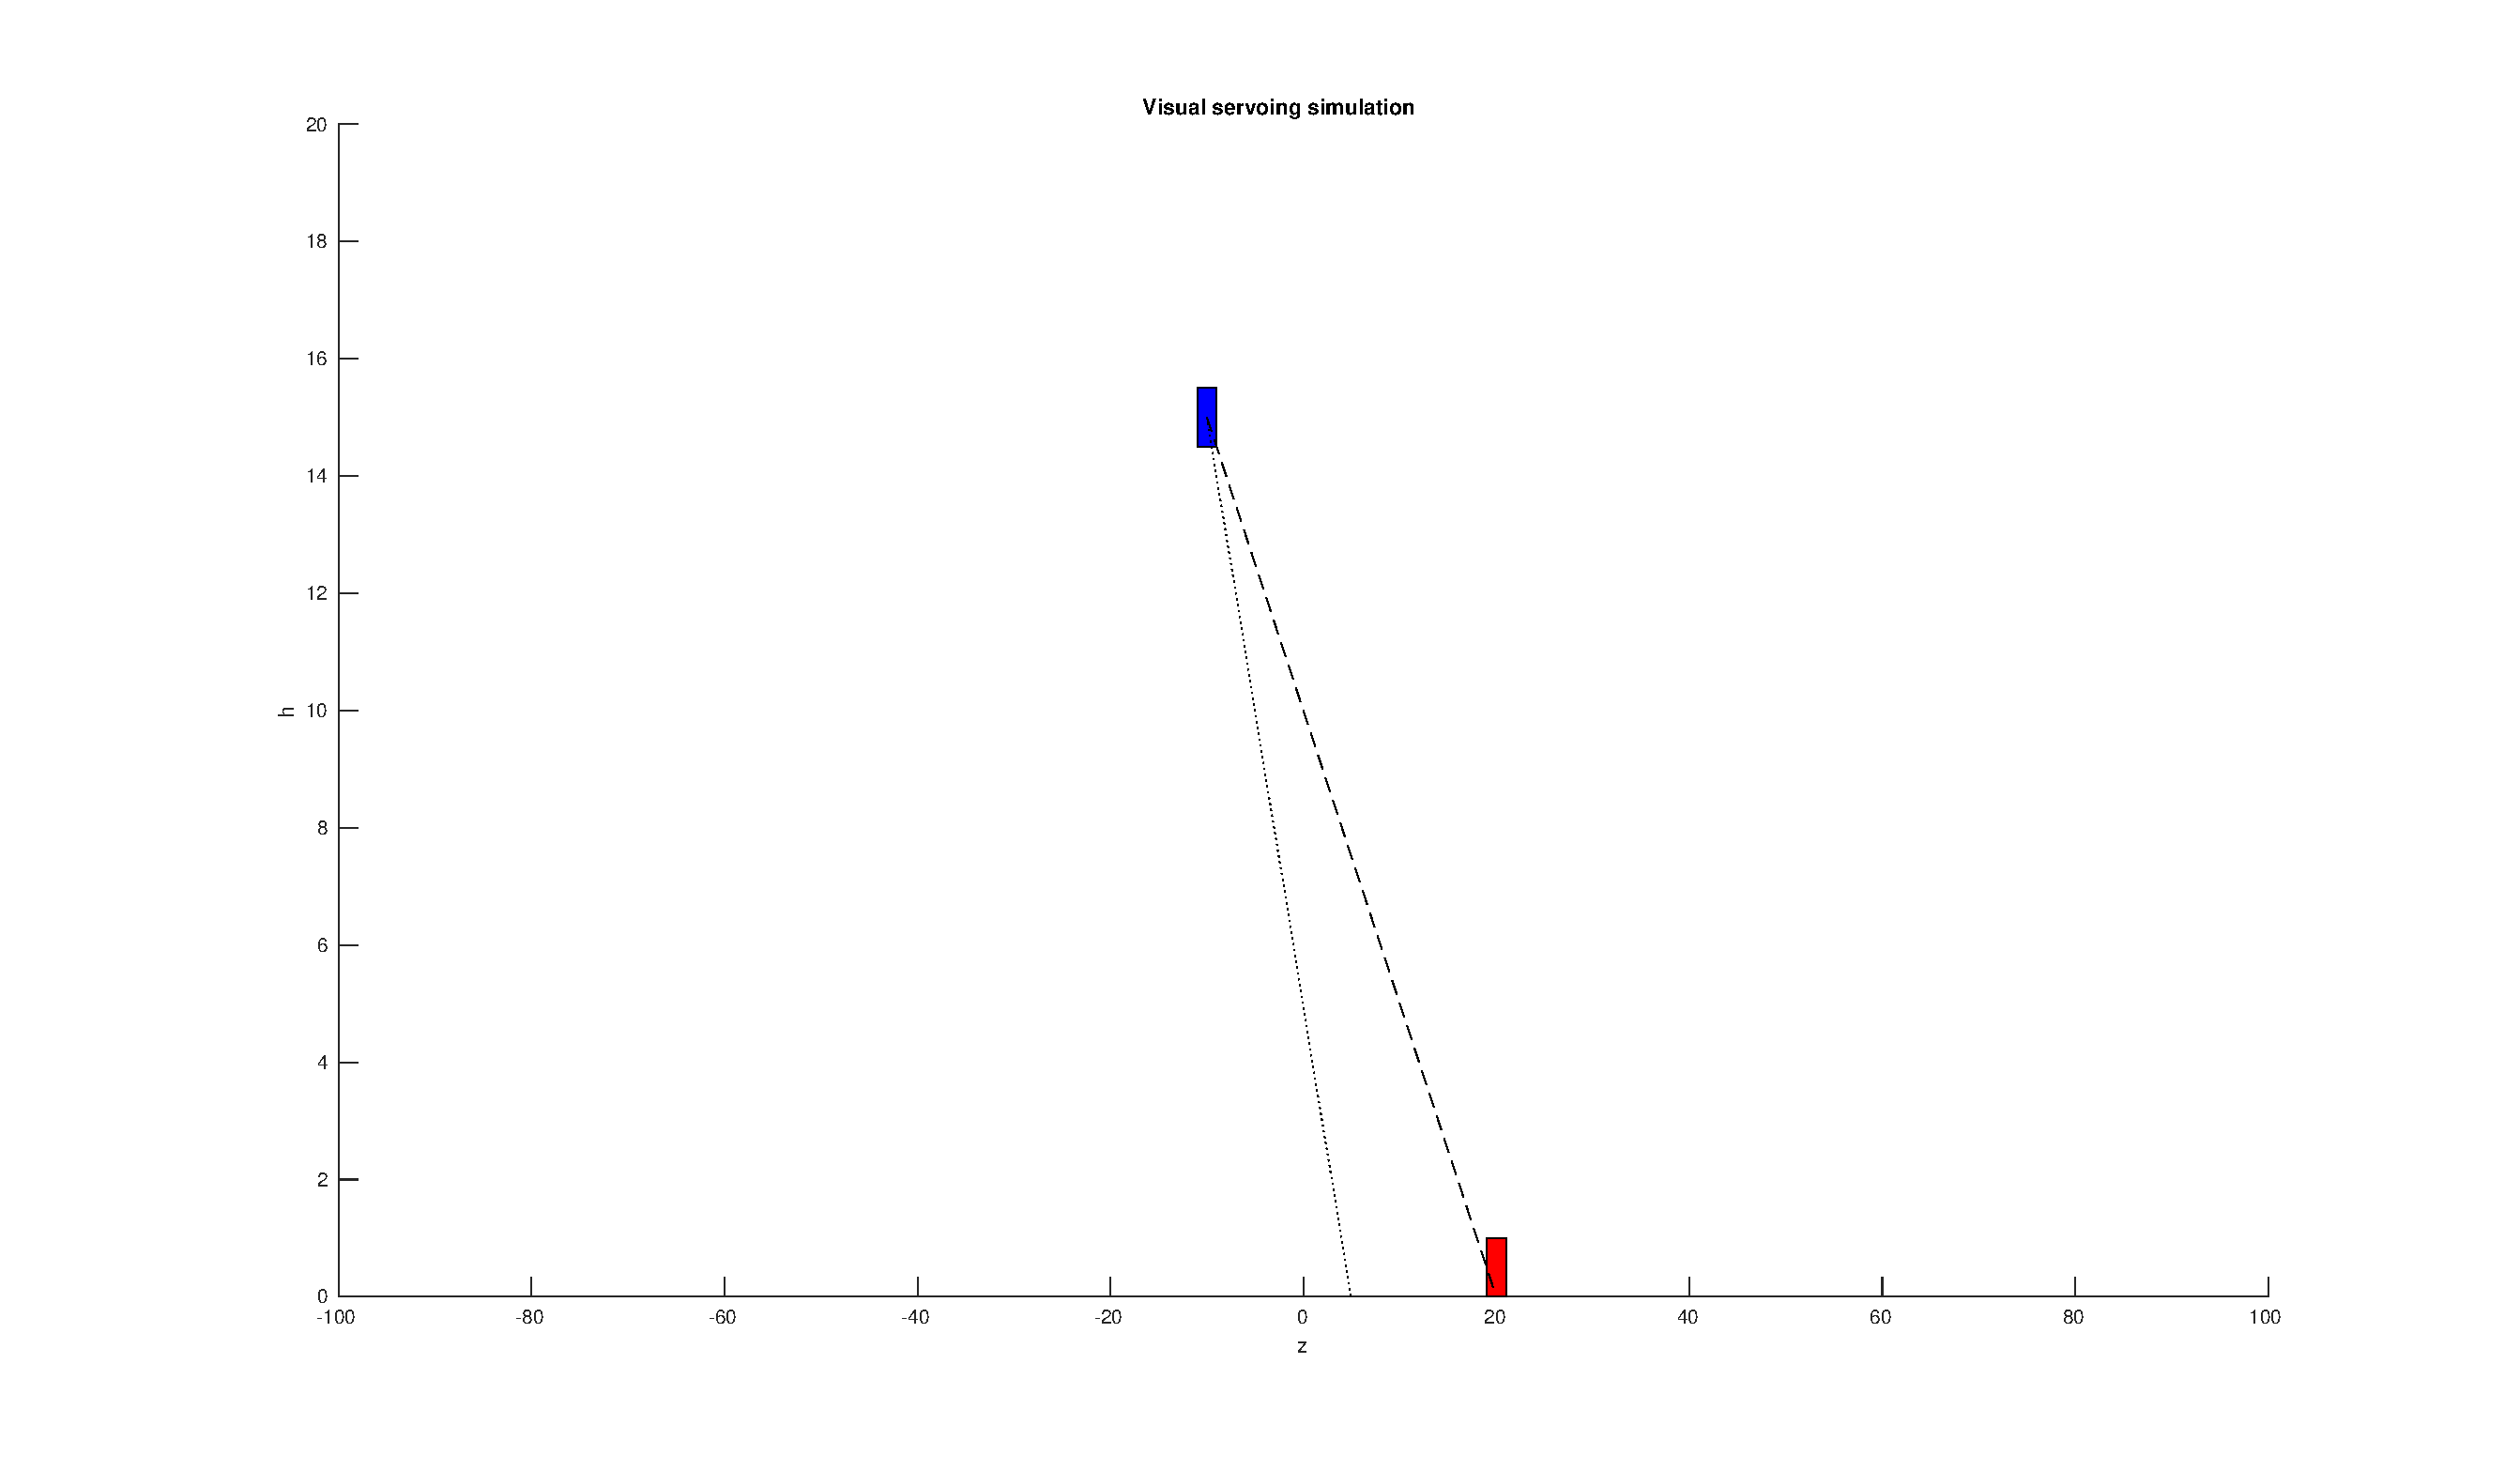
\includegraphics[width=\textwidth]{images/chapter4/simple_zero}
		\caption{when $t=0s$}
	\end{subfigure}
	~ %add desired spacing between images, e. g. ~, \quad, \qquad, \hfill etc. 
	%(or a blank line to force the subfigure onto a new line)
	\begin{subfigure}[t]{0.45\linewidth}
		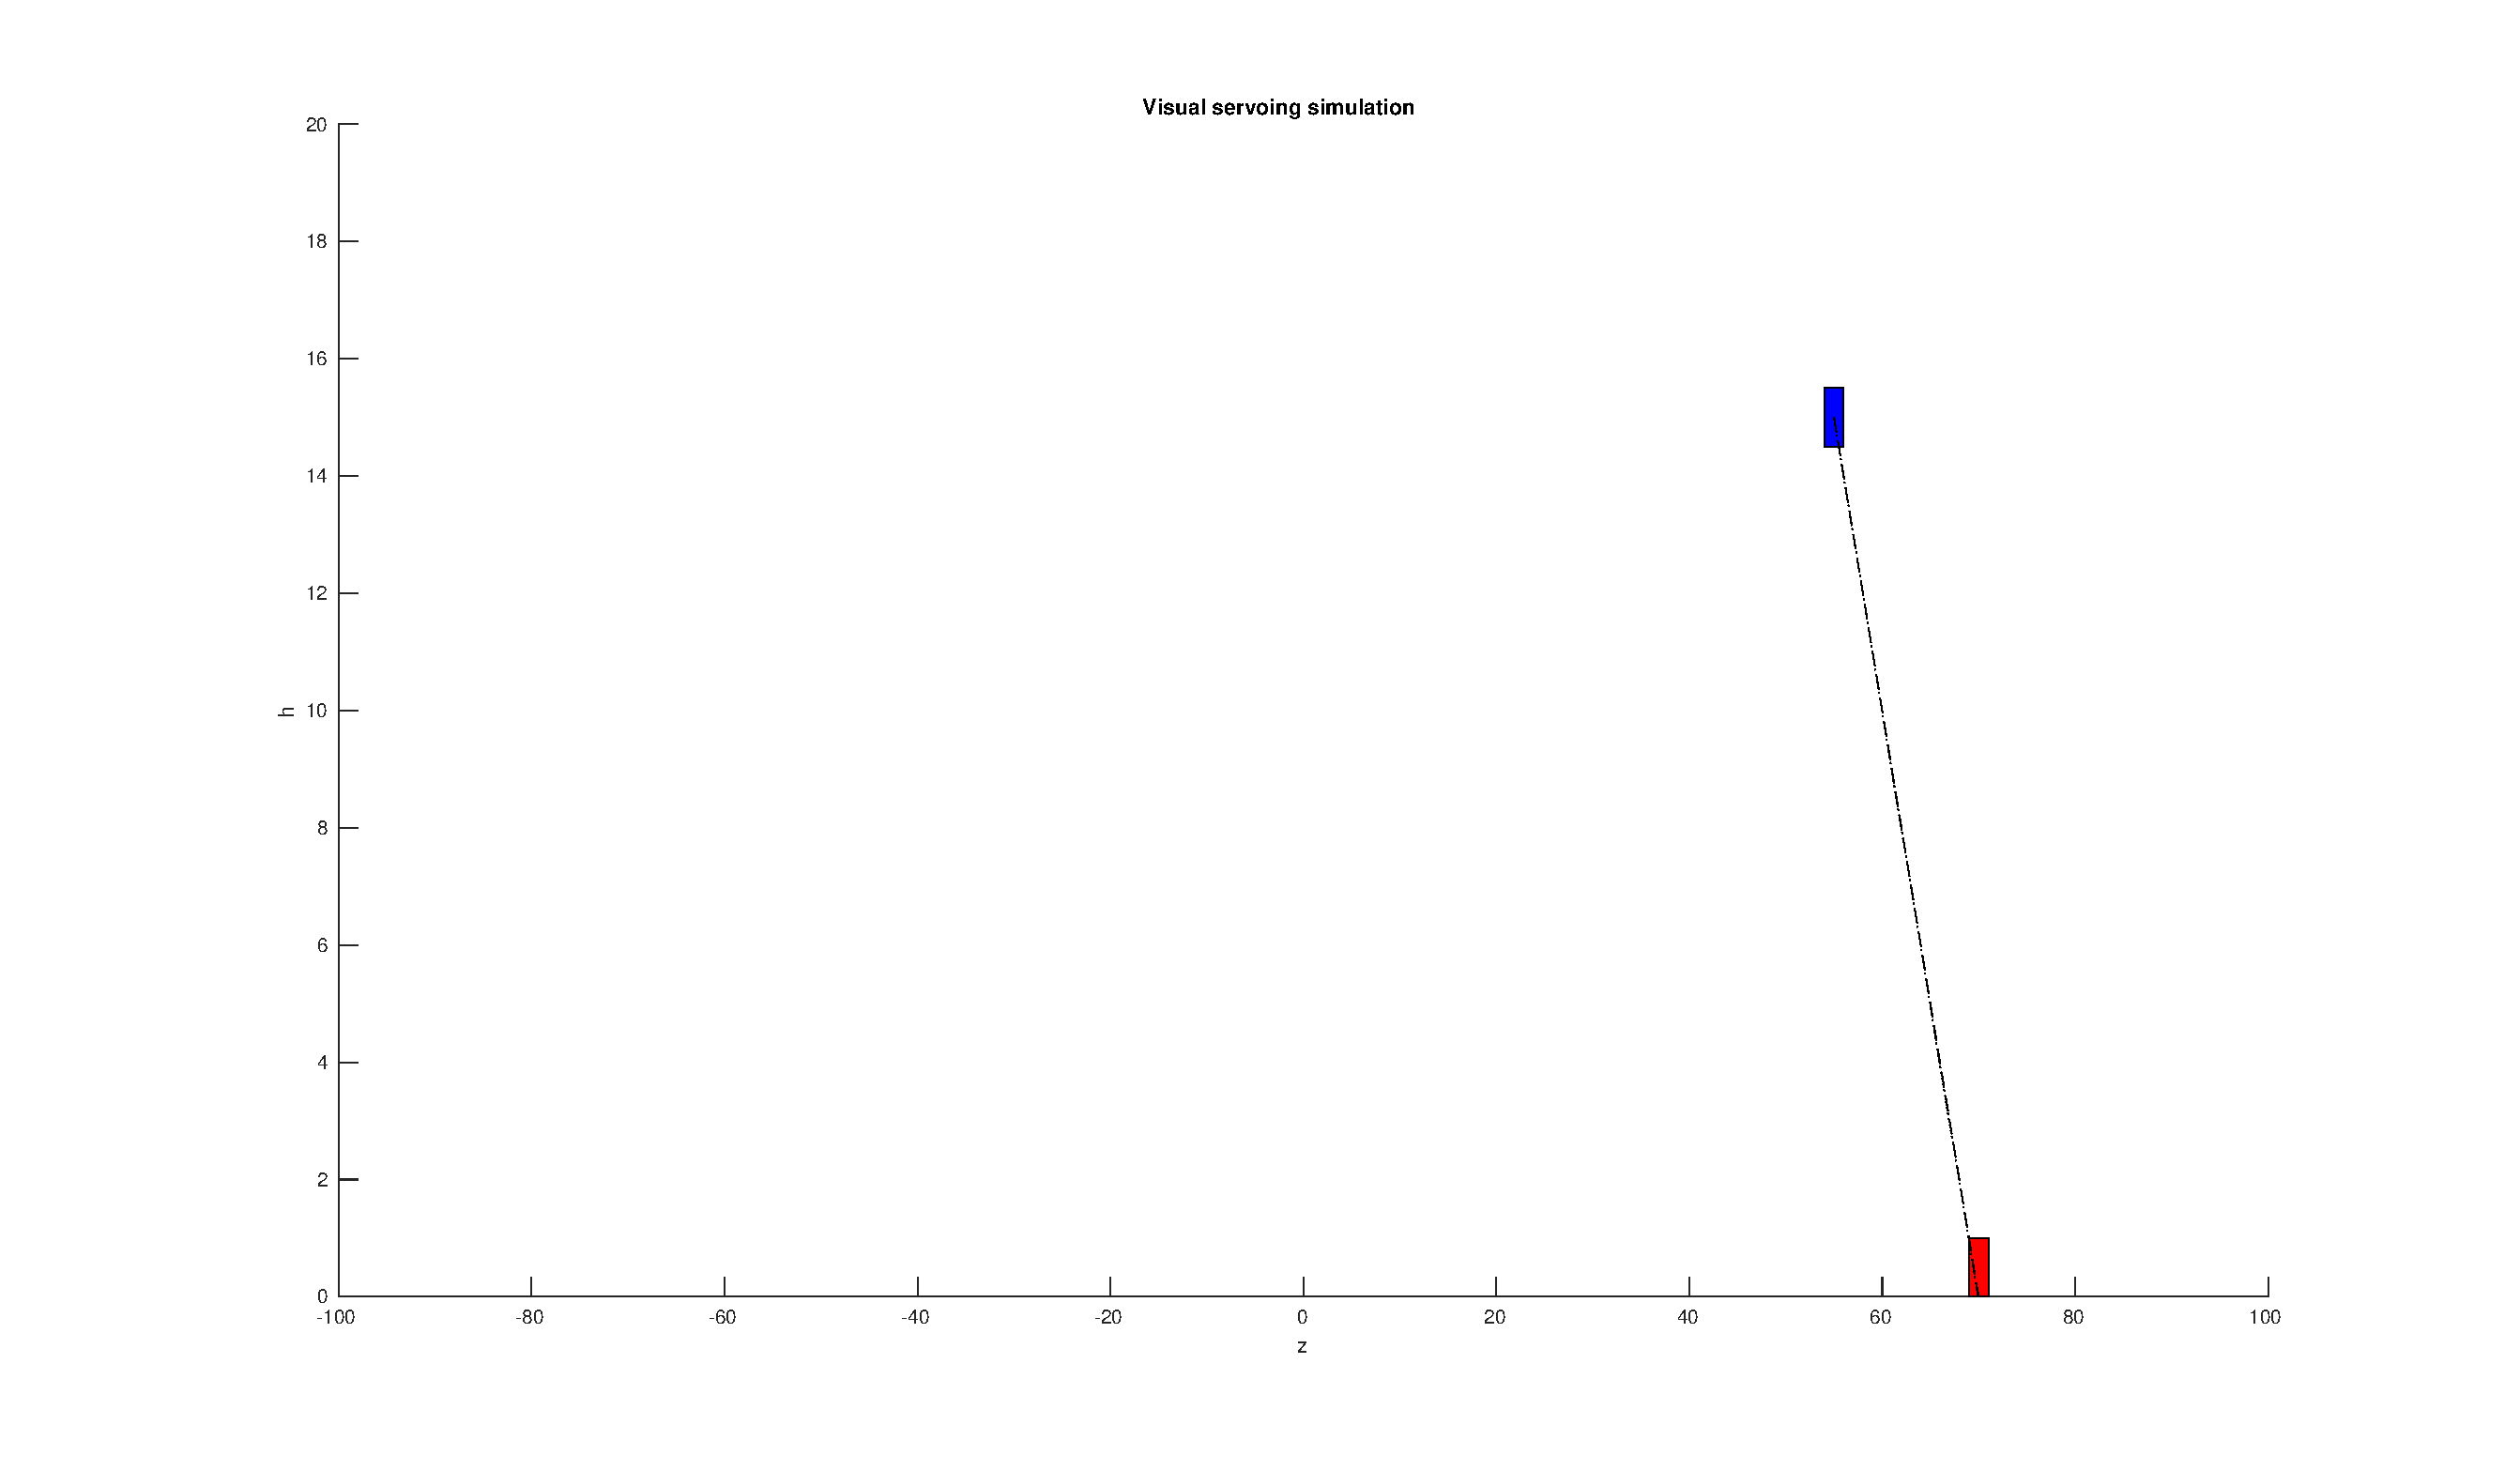
\includegraphics[width=\textwidth]{images/chapter4/simple_ten}
		\caption{when $t=10s$}
	\end{subfigure}
	\begin{subfigure}[t]{0.8\linewidth}
		\centering
		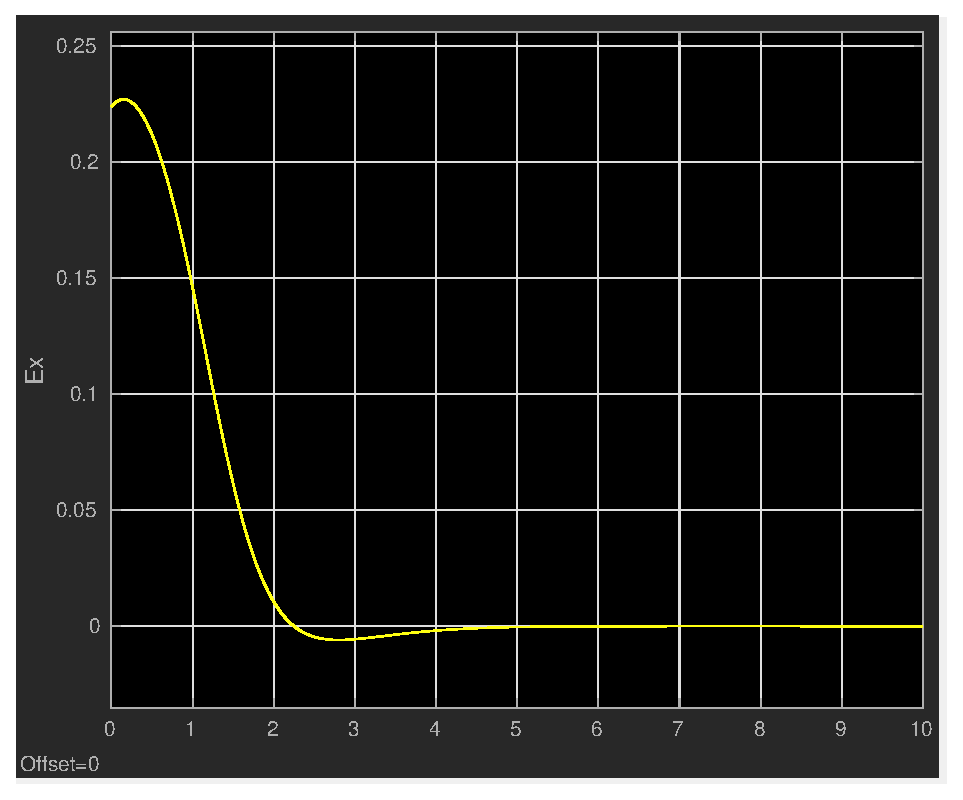
\includegraphics[width=0.5\textwidth]{images/chapter4/simple_ex}
		\caption{The horizontal error between the unit LOS vector and the unit optical axis vector converges to zero.}
	\end{subfigure}	
	\caption{Simple UAV dynamics visual servoing Simulink simulation. The blue square is flying UAV at constant altitude and the red square is a target on the ground moving at $5m/s$. The initial UAV and target positions are [-10, 15] and [20, 0] respectively. Tuning parameters are set to $k=1$, $\Gamma=I_3$ (identity matrix), and $\alpha=1000$.}
	\label{simple_simulation}
\end{figure}

\begin{figure}[htbp]
	\centering
	\begin{subfigure}[t]{0.45\linewidth}
		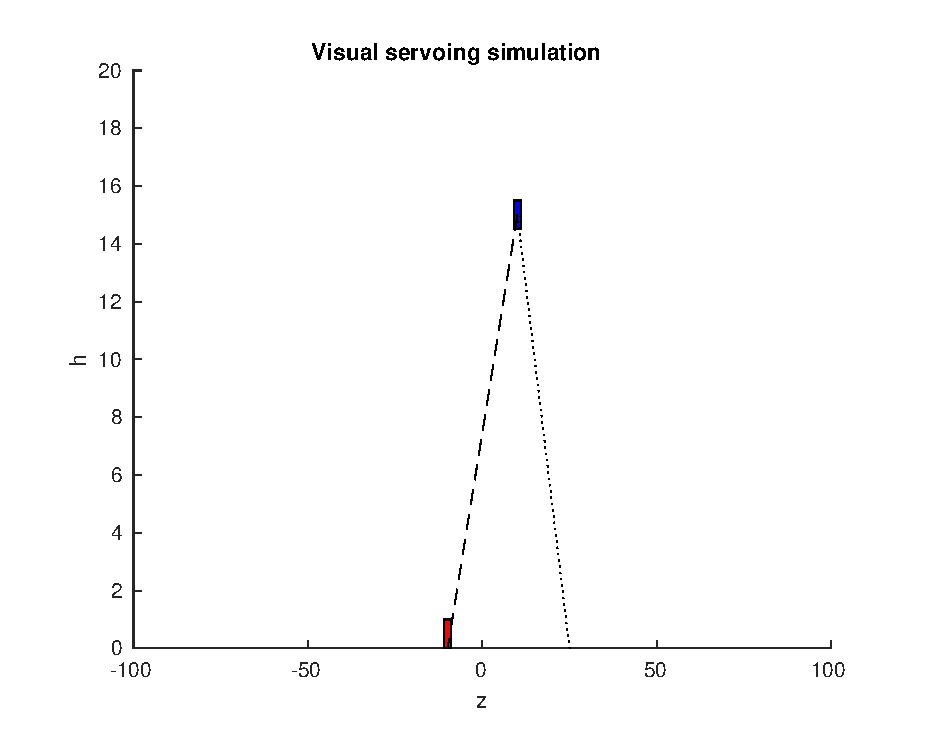
\includegraphics[width=\textwidth]{images/chapter4/another_simple_zero}
		\caption{when $t=0s$}
	\end{subfigure}
	~ %add desired spacing between images, e. g. ~, \quad, \qquad, \hfill etc. 
	%(or a blank line to force the subfigure onto a new line)
	\begin{subfigure}[t]{0.45\linewidth}
		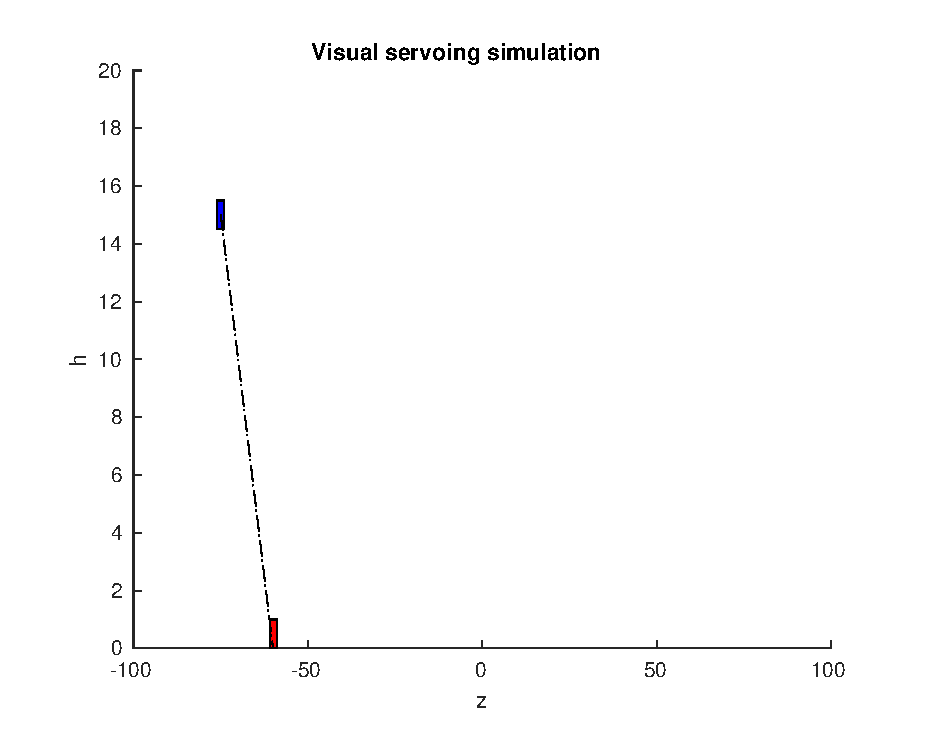
\includegraphics[width=\textwidth]{images/chapter4/another_simple_ten}
		\caption{when $t=10s$}
	\end{subfigure}
	\begin{subfigure}[t]{0.8\linewidth}
		\centering
		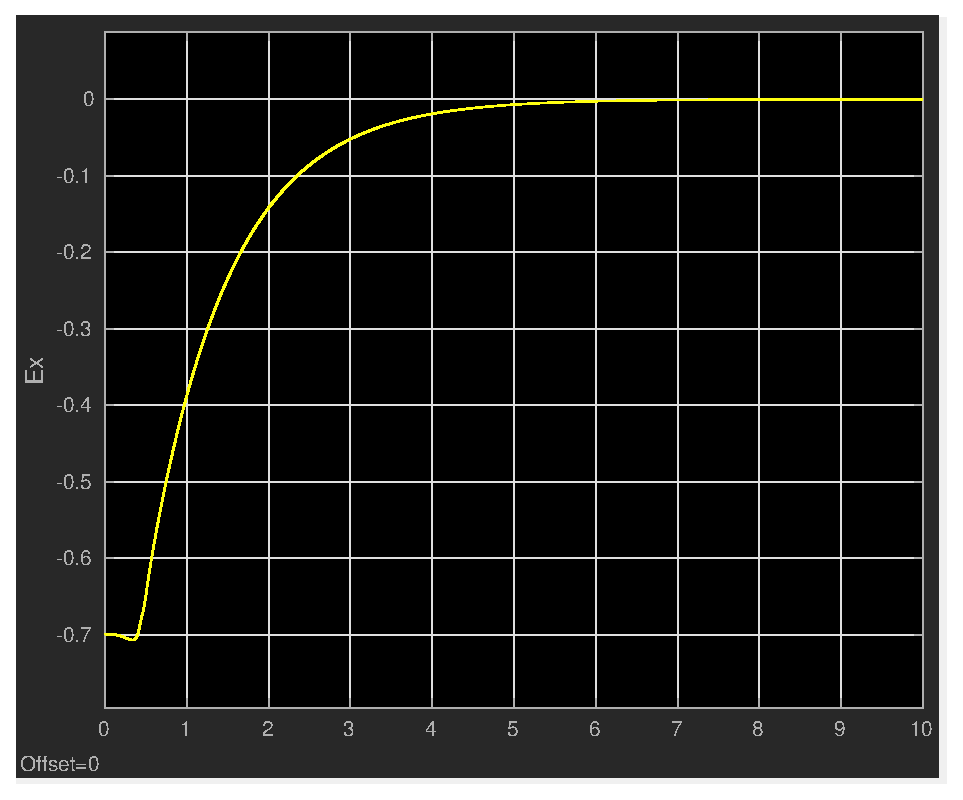
\includegraphics[width=0.5\textwidth]{images/chapter4/another_simple_ex}
		\caption{The horizontal error between the unit LOS vector and the unit optical axis vector converges to zero.}
	\end{subfigure}	
	\caption{Simple UAV dynamics visual servoing Simulink simulation. The blue square is flying UAV at constant altitude and the red square is a target on the ground moving at $-5m/s$. The initial UAV and target positions are [10, 15] and [-10, 0] respectively. Tuning parameters are set to $k=1$, $\Gamma=I_3$ (identity matrix), and $\alpha=1000$.}
	\label{another_simple_simulation}
\end{figure}


\section{Backstepping Controller Derivation for Multirotor Dynamics}
\subsection{Derivation}
The multirotor dynamics expressed in vehicle-1 frame \cite{Beard2008} is given by 
\begin{equation}
\ddot{p}_x=-\cos\phi\sin\theta\frac{F}{m}
\label{pxddot}
\end{equation}
\begin{equation}
\ddot{p}_y=\sin\phi\frac{F}{m}
\end{equation}
\begin{equation}
\ddot{p}_z=g-\cos\phi\cos\theta\frac{F}{m}
\end{equation}
\begin{equation}
\ddot{\phi}=\frac{1}{J_x}\tau_{\phi}
\end{equation}
\begin{equation}
\ddot{\theta}=\frac{1}{J_y}\tau_{\theta}
\label{thetaddot}
\end{equation}
\begin{equation}
\ddot{\psi}=\frac{1}{J_z}\tau_{\psi}
\end{equation}
where $m$ is the mass of multirotor and $J_x$, $J_y$, and, $J_z$ are the moments of inertia. Also, $F$ and $\tau$ are force and torque produced by the propellers. For our specific control interest, we are only concerned with forward and backward motion of the multirotor involving only the equation (\ref{pxddot}) and (\ref{thetaddot}). We also assume that the altitude of the multirotor is controlled with a separate altitude controller and the roll of multirotor, $\phi$, is controlled to be zero which means that the multirotor is restricted from moving sideways. When the target moves left or right, the multirotor yaws to keep the target in the camera's view and it is assumed that there is a controller for this. Applying the above conditions and using small angle approximation to linearize, the equation (\ref{pxddot}) becomes 
\begin{equation}
\ddot{p}_x=-\frac{F_e}{m}\theta
\end{equation}
where $F_e$ is the force to keep the multirotor in a constant altitude hover when the roll and pitch angles are zero. The line of sight vector is given by 
\begin{equation}
l=\begin{pmatrix}
p_x^{tar} \\ 0 \\ 0
\end{pmatrix}
-\begin{pmatrix}
p_x^{uav} \\ 0 \\ p_z^{uav}
\end{pmatrix}.
\label{l}
\end{equation}
Differentiating (\ref{l}) we get
\begin{equation}
\dot{l}=\begin{pmatrix}
\dot{p}_x^{tar} \\ 0 \\ 0
\end{pmatrix}
-\begin{pmatrix}
\dot{p}_x^{uav} \\ 0 \\ \dot{p}_z^{uav}
\end{pmatrix},
\label{ldot}
\end{equation}
and 
\begin{equation}
\ddot{l}=\begin{pmatrix}
\ddot{p}_x^{tar} \\ 0 \\ 0
\end{pmatrix}
-\begin{pmatrix}
\ddot{p}_x^{uav} \\ 0 \\ \ddot{p}_z^{uav}
\end{pmatrix}.
\label{lddot1}
\end{equation}
Referring back to (\ref{p_mhat}), (\ref{e_1}) and (\ref{lddot1}) we get that  
\begin{align}
\hat{e}_1^{\top}P_{\hat{m}}\ddot{l}&=(1-m_1^2)(\ddot{p}_x^{tar}-\ddot{p}_x^{uav})+m_1m_2\ddot{p}_z^{uav}
\\&=(1-m_1^2)\frac{F_e}{m}\theta
\end{align}
assuming that the multirotor keeps its altitude constant and the target does not accelerate. Notice that 
\begin{equation}
P_{\hat{m}}=\begin{pmatrix}1-m_1^2 & 0 & -m_1m_2 \\ 0 & 1 & 0 \\ -m_1m_2 & 0 & 1-m_2^2 \end{pmatrix}
\end{equation}
which is different from (\ref{p_mhat}) because now the $z$ component of the optical axis unit vector in vehicle-1 frame aligns with $z$ axis of the vehicle-1 frame (i.e. NED coordinate frame). However, this turns out to not affect the controller derivation.  Again, the control objective is to drive $e_x$ to zero and this can be achieved by driving $s=\dot{e_x}+ke_x$ to zero.
Recalling (\ref{exddot}) we get
\begin{align}
\ddot{e}_x&=\frac{1}{L}(1-m_1^2)\frac{F_e}{m}\theta+\frac{\dot{L}}{L}(-2\hat{e}_1^{\top}P_{\hat{m}}\dot{\hat{l}})+\frac{\ddot{L}}{L}(-\hat{e}_1^{\top}P_{\hat{m}}\hat{l})
\\&=\beta_1\phi_1\frac{F_e}{m}\theta+\beta_2\phi_2+\beta_3\phi_3
\label{exddot1}
\end{align} 
where
\begin{equation}
\beta_1 \triangleq \frac{1}{L},\quad \beta_2 \triangleq \frac{\dot{L}}{L}, \quad \beta_3 \triangleq \frac{\ddot{L}}{L}
\end{equation}
and
\begin{equation}
\phi_1 \triangleq 1-m_1^2,\quad \phi_2 \triangleq -2\hat{e}_1^{\top}P_{\hat{m}}\dot{\hat{l}}, \quad \phi_3 \triangleq -\hat{e}_1^{\top}P_{\hat{m}}\hat{l}.
\end{equation}
Since we have all necessary components, we can get 
\begin{align}
\dot{s}&=\ddot{e}_x+k\dot{e}_x
\\&=\beta_1\phi_1\frac{F_e}{m}\theta+\beta_2\phi_2+\beta_3\phi_3+k\dot{e}_x.
\label{sdot3}
\end{align}
Manipulating (\ref{sdot3}) yields
\begin{align}
\dot{s}&=\beta_1\phi_1\frac{F_e}{m}\theta+\beta_2\phi_2+\beta_3\phi_3+k\dot{e_x}+\hat{\beta}_1\phi_1\frac{F_e}{m}\theta+\hat{\beta}_2\phi_2+\hat{\beta}_3\phi_3-\hat{\beta}_1\phi_1\frac{F_e}{m}\theta-\hat{\beta}_2\phi_2-\hat{\beta}_3\phi_3
\\&=(\beta_1-\hat{\beta}_1)\phi_1\frac{F_e}{m}\theta+(\beta_2-\hat{\beta}_2)\phi_2+(\beta_3-\hat{\beta}_3)\phi_3+k\dot{e_x}+\hat{\beta}_1\phi_1\frac{F_e}{m}\theta+\hat{\beta}_2\phi_2+\hat{\beta}_3\phi_3
\\&=\tilde{\beta}_1\phi_1\frac{F_e}{m}\theta+\tilde{\beta}_2\phi_2+\tilde{\beta}_3\phi_3+k\dot{e_x}+\hat{\beta}_1\phi_1\frac{F_e}{m}\theta+\hat{\beta}_2\phi_2+\hat{\beta}_3\phi_3
\\&=\tilde{B}^\top\Phi+k\dot{e_x}+\hat{\beta}_1\phi_1\frac{F_e}{m}\theta+\hat{\beta}_2\phi_2+\hat{\beta}_3\phi_3
\end{align}
where 
\begin{equation}
B \triangleq \begin{pmatrix}
\beta_1 \\ \beta_2 \\ \beta_3
\end{pmatrix}, \quad
\hat{B} \triangleq \begin{pmatrix} \hat{\beta}_1 \\ \hat{\beta}_2 \\ \hat{\beta}_3 \end{pmatrix}, \quad
\tilde{B} \triangleq B-\hat{B}, \quad 
\Phi \triangleq \begin{pmatrix} \phi_1\frac{F_e}{m}\theta \\ \phi_2 \\ \phi_3 \end{pmatrix}.
\end{equation}
Define the Lyapunov function candidate as
\begin{equation}
V_1=\frac{1}{2}s^2+\frac{1}{2}\tilde{B}^\top \Gamma^{-1}\tilde{B}
\label{v1}
\end{equation}
and take the derivative to get
\begin{align}
\dot{V}_1&=s\dot{s}+\tilde{B}^\top \Gamma^{-1}\dot{\tilde{B}}
\\&=s(\tilde{B}^\top\Phi+k\dot{e_x}+\hat{\beta}_1\phi_1\frac{F_e}{m}\theta+\hat{\beta}_2\phi_2+\hat{\beta}_3\phi_3)+\tilde{B}^\top \Gamma^{-1}\dot{\tilde{B}}
\\&=s(k\dot{e_x}+\hat{\beta}_1\phi_1\frac{F_e}{m}\theta+\hat{\beta}_2\phi_2+\hat{\beta}_3\phi_3)+s\tilde{B}^\top\Phi+\tilde{B}^\top \Gamma^{-1}\dot{\tilde{B}}.
\label{sdot4}
\end{align}
Assuming that $B$ is constant or slowly changing, then $\dot{\tilde{B}}=-\dot{\hat{B}}$, and equation (\ref{sdot4}) becomes 
\begin{equation}
\dot{V}_1=s(k\dot{e_x}+\hat{\beta}_1\phi_1\frac{F_e}{m}\theta+\hat{\beta}_2\phi_2+\hat{\beta}_3\phi_3)+s\tilde{B}^\top\Phi-\tilde{B}^\top \Gamma^{-1}\dot{\hat{B}}.
\end{equation}
By selecting $\dot{\hat{B}}=s\Gamma\Phi$, the above equation further becomes 
\begin{equation}
\dot{V}_1=s(k\dot{e_x}+\hat{\beta}_1\phi_1\frac{F_e}{m}\theta+\hat{\beta}_2\phi_2+\hat{\beta}_3\phi_3).
\label{v1dot}
\end{equation}
For some cases, $\theta$ is the direct control input that can be commanded making the problem less complicated. However, for the multirotor dynamics, $\theta$ is indirectly controlled by torque $\tau_\theta$ which leads to the development of backstepping control technique. The backstepping control is especially useful when the system has cascaded structure such as this multirotor case by using some of the state variables as pseudo controls to backstep until the final external control input is reached. With backstepping, a Lyapunov function is derived for the entire system \cite{khalil1996noninear}, \cite{raptis2010linear}. We start by adding and subtracting a pseudo control $\xi_1$ to equation (\ref{v1dot}) as
\begin{equation}
\dot{V}_1=s(k\dot{e_x}+\hat{\beta}_1\phi_1\frac{F_e}{m}\theta+\hat{\beta}_2\phi_2+\hat{\beta}_3\phi_3+\xi_1-\xi_1).
\end{equation}
By selecting $\xi_1=-k\dot{e}_x-\hat{\beta}_2\phi_2-\hat{\beta}_3\phi_3-k_1s$, 
\begin{equation}
\dot{V}_1=-k_1s^2+ s(\hat{\beta}_1\phi_1\frac{F_e}{m}\theta-\xi_1).
\label{v2dot}
\end{equation}
Define a new Lyapunov function candidate as
\begin{equation}
V_2=V_1+\frac{1}{2}(\hat{\beta}_1\phi_1\frac{F_e}{m}\theta-\xi_1)^2,
\label{v2}
\end{equation}
and taking derivative, we get
\begin{align}
\dot{V}_2&=\dot{V}_1+(\hat{\beta}_1\phi_1\frac{F_e}{m}\theta-\xi_1)(\phi_1\frac{F_e}{m}(\dot{\hat{\beta}}_1\theta+\hat{\beta}_1\dot{\theta})-\dot{\xi}_1)
\\&=-k_1s^2+
(\hat{\beta}_1\phi_1\frac{F_e}{m}\theta-\xi_1)
(s+\phi_1\frac{F_e}{m}(\dot{\hat{\beta}}_1\theta+\hat{\beta}_1\dot{\theta})-\dot{\xi}_1+\xi_2-\xi_2).
\end{align}
Assigning $\xi_2=\dot{\xi}_1-s-\phi_1\frac{F_e}{m}\dot{\hat{\beta}}_1\theta-k_2(\hat{\beta}_1\phi_1\frac{F_e}{m}\theta-\xi_1)$ leads to
\begin{equation}
\dot{V}_2=-k_1s^2-k_2(\hat{\beta}_1\phi_1\frac{F_e}{m}\theta-\xi_1)^2+
(\hat{\beta}_1\phi_1\frac{F_e}{m}\theta-\xi_1)
(\phi_1\frac{F_e}{m}\hat{\beta}_1\dot{\theta}-\xi_2).
\label{v2dotfinal}
\end{equation}
Finally, define a new Lyapunov function as 
\begin{equation}
V_3=V_2+\frac{1}{2}(\phi_1\frac{F_e}{m}\hat{\beta}_1\dot{\theta}-\xi_2)^2,
\label{v3}
\end{equation}
and differentiate to get
\begin{align}
\dot{V}_3&=\dot{V}_2+
(\phi_1\frac{F_e}{m}\hat{\beta}_1\dot{\theta}-\xi_2)
(\phi_1\frac{F_e}{m}\dot{\hat{\beta}}_1\dot{\theta}+\phi_1\frac{F_e}{m}\hat{\beta}_1\ddot{\theta}-\dot{\xi}_2)
\\&=-k_1s^2-k_2(\hat{\beta}_1\phi_1\frac{F_e}{m}\theta-\xi_1)^2+(\phi_1\frac{F_e}{m}\hat{\beta}_1\dot{\theta}-\xi_2)
(\hat{\beta}_1\phi_1\frac{F_e}{m}\theta-\xi_1+\phi_1\frac{F_e}{m}\dot{\hat{\beta}}_1\dot{\theta}+\phi_1\frac{F_e}{m}\hat{\beta}_1\ddot{\theta}-\dot{\xi}_2).
\label{v3dot}
\end{align}
 Using the relationship between the angular acceleration and torque in (\ref{thetaddot}), the above equation becomes
\begin{equation}
\dot{V}_3=-k_1s^2-k_2(\hat{\beta}_1\phi_1\frac{F_e}{m}\theta-\xi_1)^2+(\phi_1\frac{F_e}{m}\hat{\beta}_1\dot{\theta}-\xi_2)
(\hat{\beta}_1\phi_1\frac{F_e}{m}\theta-\xi_1+\phi_1\frac{F_e}{m}\dot{\hat{\beta}}_1\dot{\theta}+\phi_1\frac{F_e}{m}\hat{\beta}_1\frac{1}{J_y}\tau_\theta-\dot{\xi}_2)
\label{v3dotfinal}
\end{equation}
Notice that $\tau_\theta$ finally showed up in the equation (\ref{v3dotfinal}) which we can directly control. Thus, by setting 
\begin{equation}
\tau_\theta=\frac{J_ym}{\phi_1F_e\hat{\beta}_1}
(\xi_1+\dot{\xi}_2-\hat{\beta}_1\phi_1\frac{F_e}{m}\theta-\phi_1\frac{F_e}{m}\dot{\hat{\beta}}_1\dot{\theta}-k_3(\phi_1\frac{F_e}{m}\hat{\beta}_1\dot{\theta}-\xi_2)),
\end{equation}
gives
\begin{equation}
\dot{V}_3=-k_1s^2-k_2(\hat{\beta}_1\phi_1\frac{F_e}{m}\theta-\xi_1)^2-k_3(\phi_1\frac{F_e}{m}\hat{\beta}_1\dot{\theta}-\xi_2)^2.
\end{equation}
Because of the cascaded structure of the backstepping control, the fact that $V_3(t)\rightarrow 0$ means that $V_1(t)$ also converges to zero.

\subsection{Simulation}
The backstepping control algorithm derived above is simulated in Simulink with more realistic multirotor dynamics that can be found in {\cite{Beard2008}}. The simulation only tests the forward motion control of the multirotor by having separate PID controller to keep roll and yaw motions unmoved. There are two types of backstepping controller tested. The first is using the inertial LOS vector and normalize it to get the unit LOS vector shown in Figure \ref{system_inertial}. This is rather unrealistic because it is usually not feasible to know the target location in inertial frame to get the inertial LOS vector. However, this is still tested as an intermediate step and is used to test the validity of the backstepping control algorithm itself. The simulation results with various target velocity $0m/s$, $5m/s$, and $-5m/s$ can be found in Figure \ref{inertial_0mps}, \ref{inertial_5mps}, and \ref{inertial_-5mps} respectively.
\begin{figure}[htbp]
	\centering
	\framebox{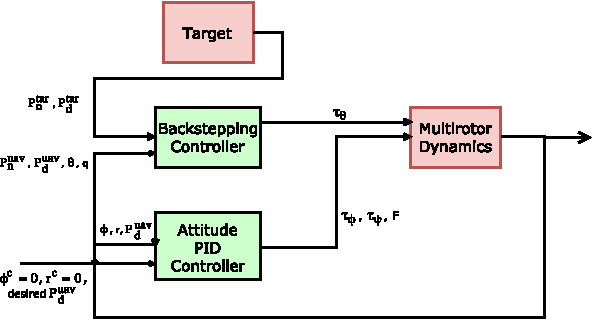
\includegraphics[width=0.8\textwidth]{images/chapter4/inertial_LOS_backstepping.pdf}}
	\caption{Control system diagram for the inertial line of sight vector backstepping controller. In this configuration, the backstepping controller needs the positions of multirotor and target.}
	\label{system_inertial}
\end{figure}

\begin{figure}[htbp]
	\centering
	\framebox{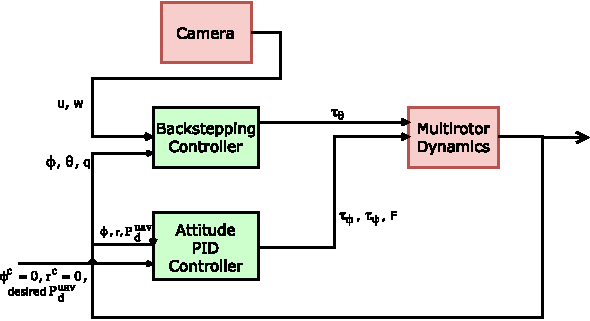
\includegraphics[width=0.8\textwidth]{images/chapter4/image_based_backstepping.pdf}}
	\caption{Control system diagram for the image-based backstepping controller. Note that the backstepping controller only requires the image coordinates of the target.}
	\label{system_image}
\end{figure}

\begin{figure}[htbp]
	\centering
	\begin{subfigure}[t]{0.45\linewidth}
		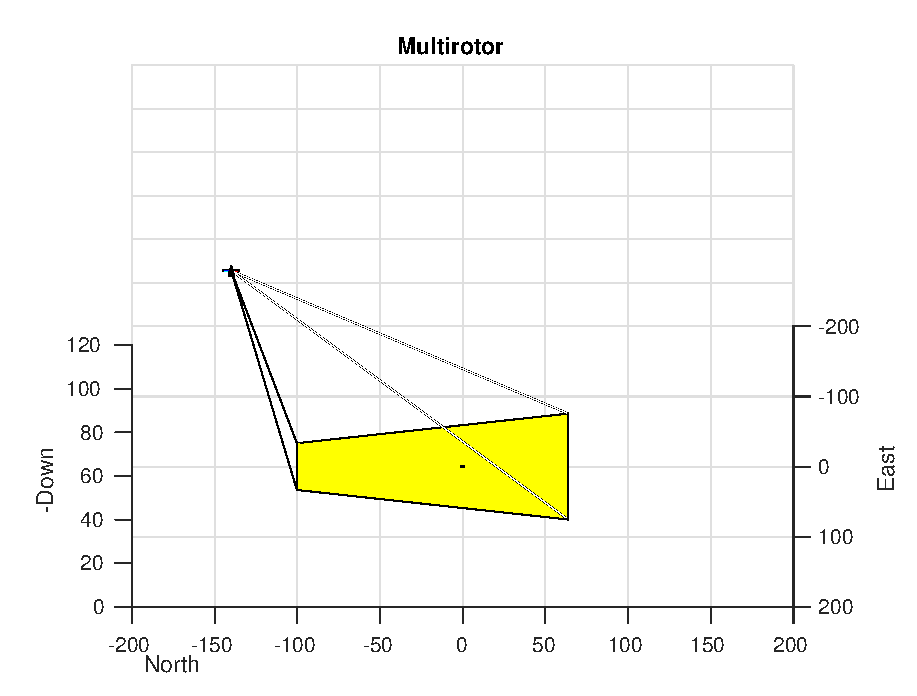
\includegraphics[width=\textwidth]{images/chapter4/inertial_UAV_0mps}
		\caption{Multirotor and ground target when $t=0s$}
	\end{subfigure}
	\begin{subfigure}[t]{0.45\linewidth}
		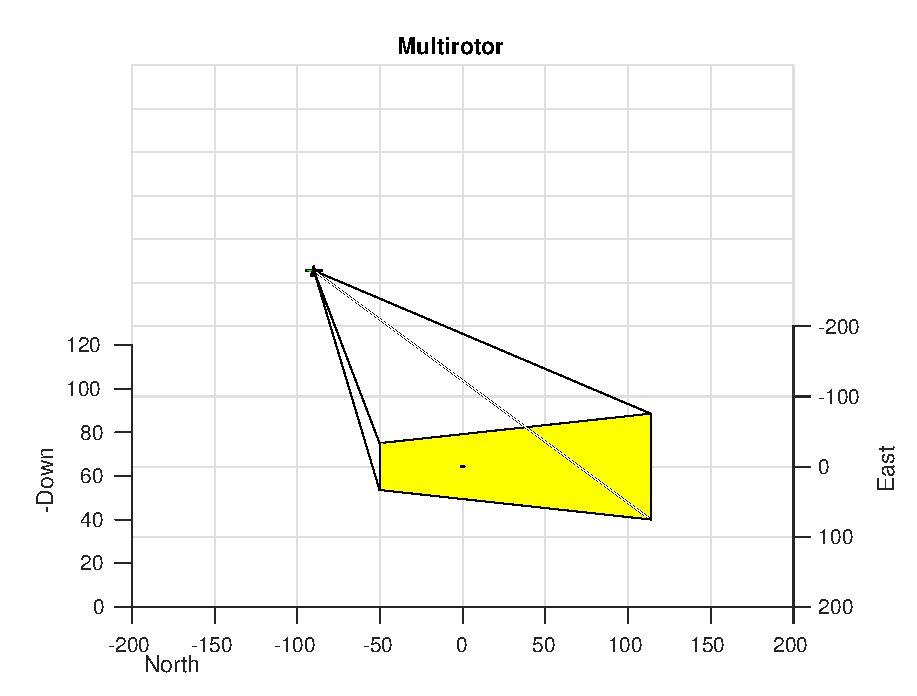
\includegraphics[width=\textwidth]{images/chapter4/inertial_UAV_0mps_60s}
		\caption{when $t=60s$}
	\end{subfigure}
	\begin{subfigure}[t]{0.45\linewidth}
		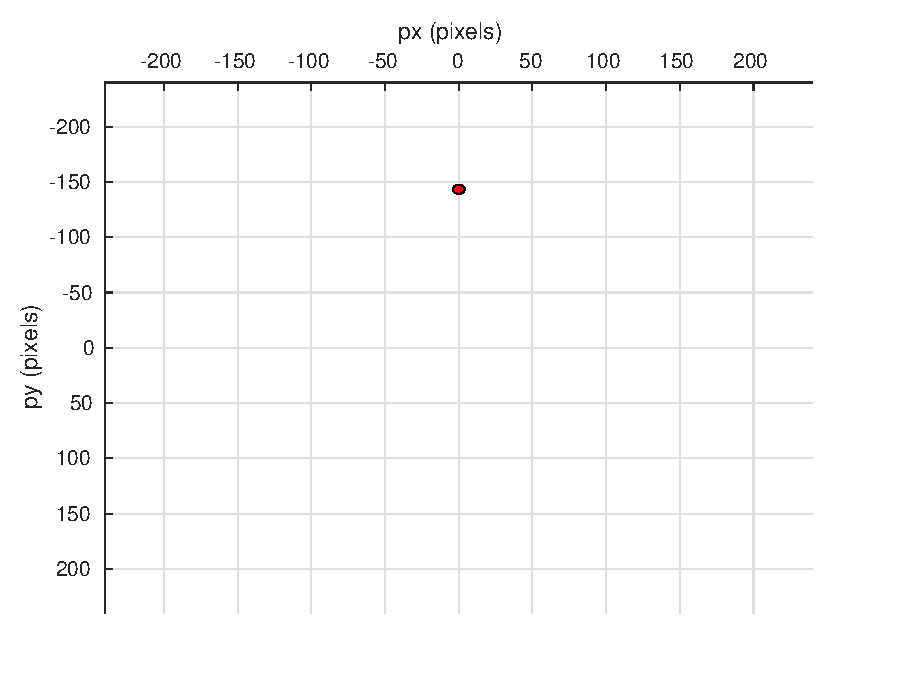
\includegraphics[width=\textwidth]{images/chapter4/inertial_camera_0mps}
		\caption{Camera view when $t=0s$}
	\end{subfigure}
	\begin{subfigure}[t]{0.45\linewidth}
		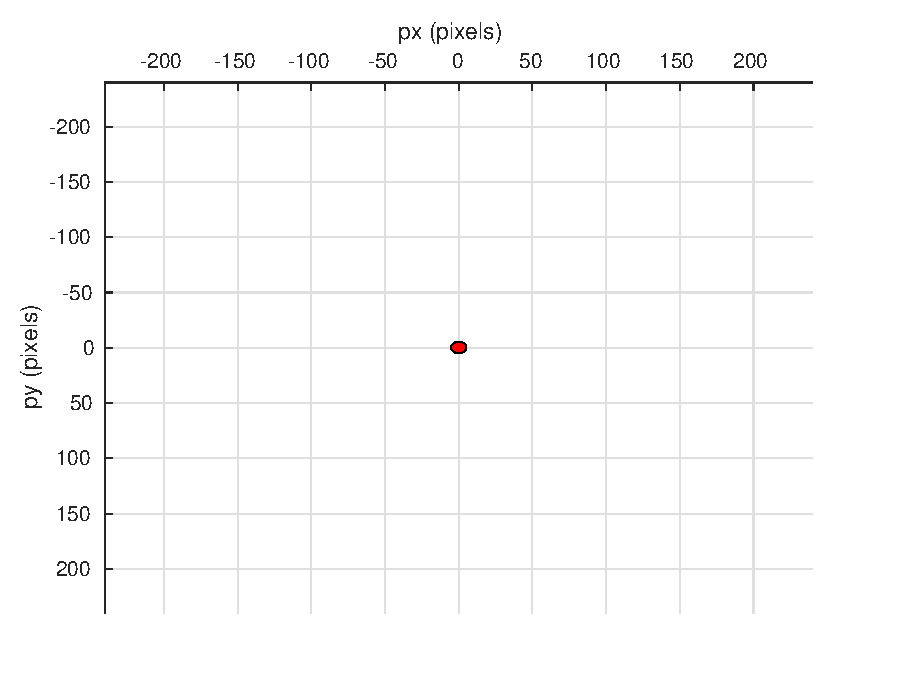
\includegraphics[width=\textwidth]{images/chapter4/inertial_camera_0mps_60s}
		\caption{when $t=60s$}
	\end{subfigure}
	\begin{subfigure}[t]{0.8\linewidth}
		\centering
		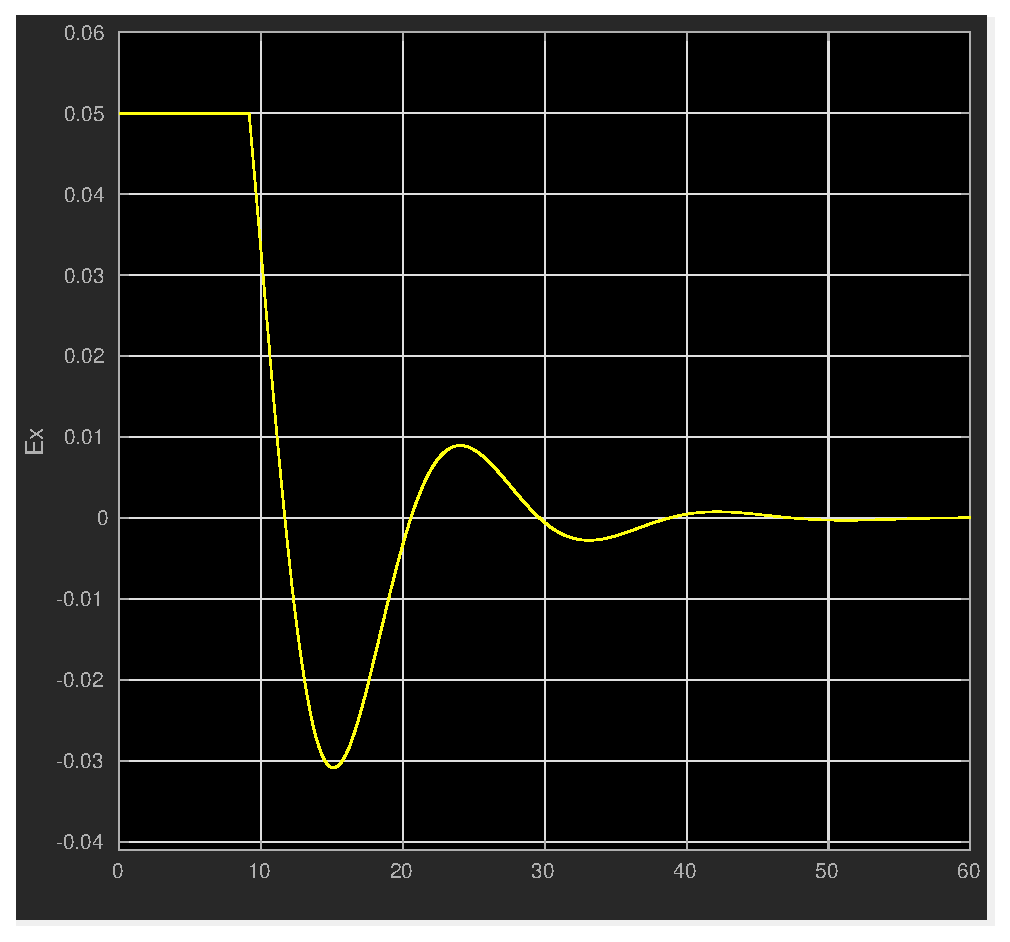
\includegraphics[width=0.5\textwidth]{images/chapter4/inertial_Ex_0mps}
		\caption{The horizontal error ($e_x$) between the unit LOS vector and the unit optical axis vector both in the vehicle-1 frame converges to zero. It saturates at 0.05 to prevent the multirotor from commanding too large torque command.}
	\end{subfigure}	
	\caption{Simulation result for the backstepping control using the inertial LOS vector. The ground target is static ($0m/s$). The initial UAV and target positions are [-140, 0, -90] and [0, 0, 0] respectively. Tuning parameters are set to $k=0.12$, $k_1=1$, $k_2=1$, $k_3=1$, and $\Gamma=0.01*I_3$ (identity matrix).}
	\label{inertial_0mps}
\end{figure}

\begin{figure}[htbp]
	\centering
	\begin{subfigure}[t]{0.32\linewidth}
		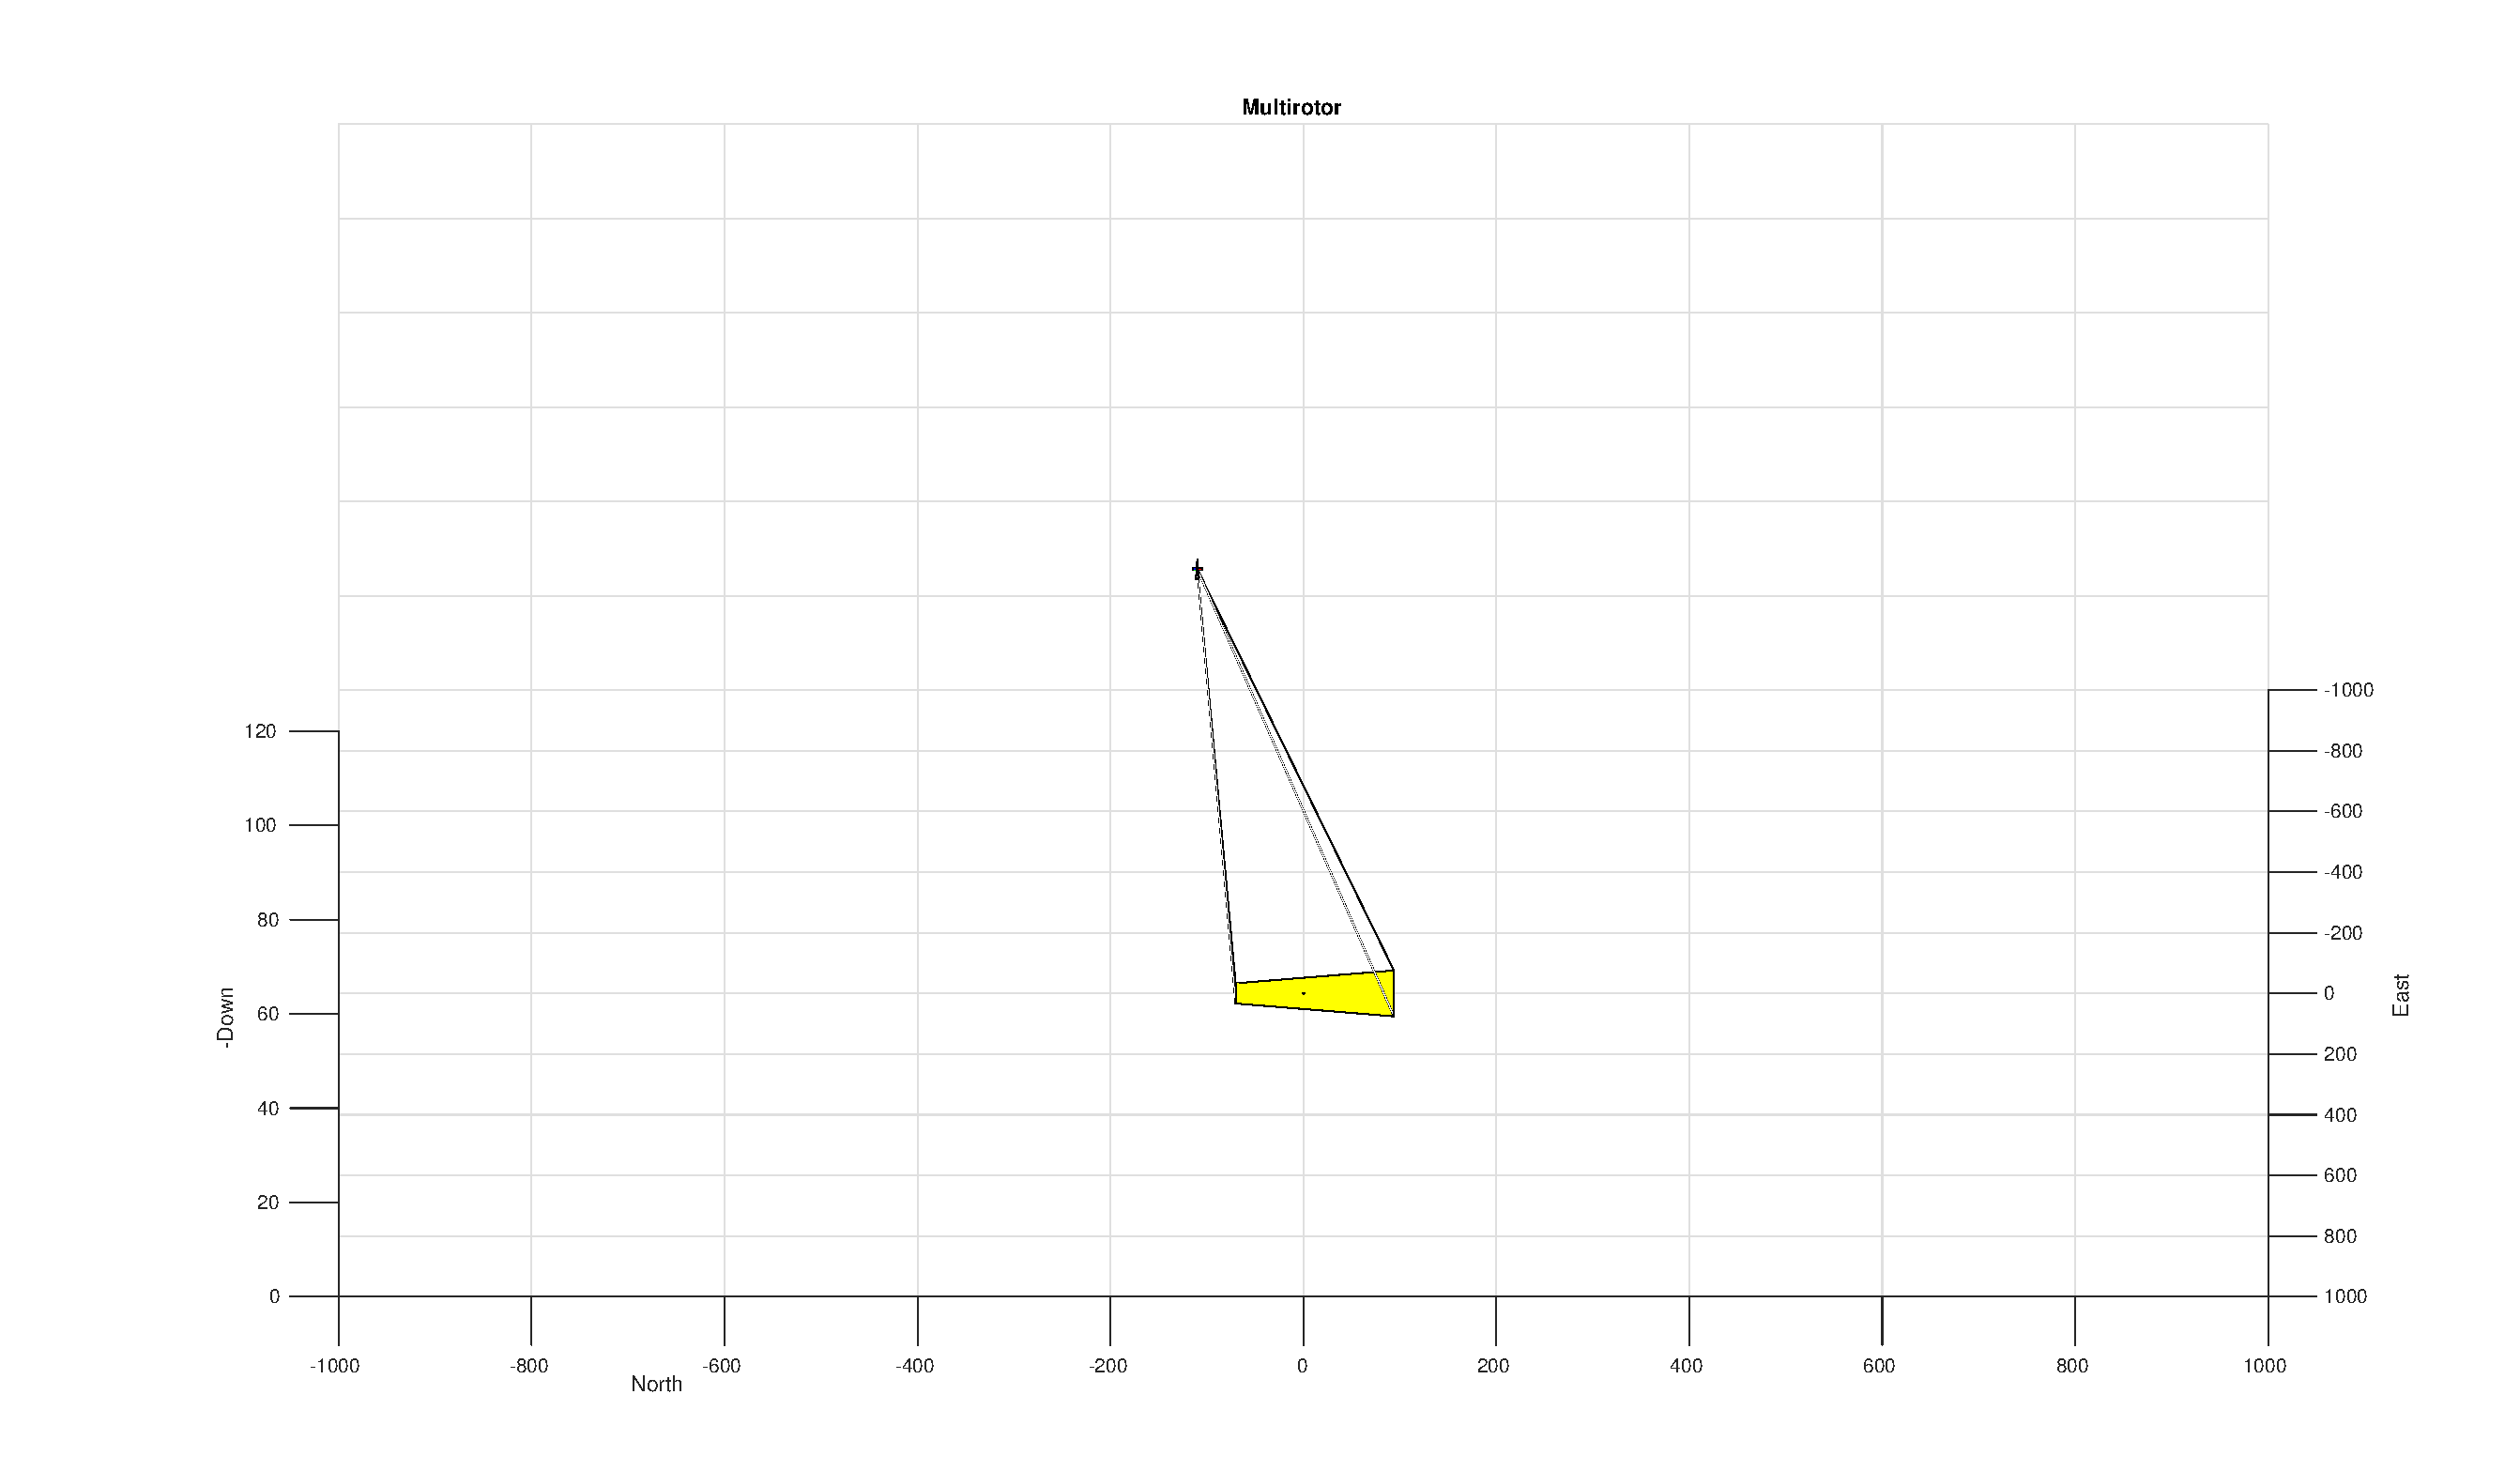
\includegraphics[width=\textwidth]{images/chapter4/inertial_UAV_5mps}
		\caption{when $t=0s$}
	\end{subfigure}
	\begin{subfigure}[t]{0.32\linewidth}
		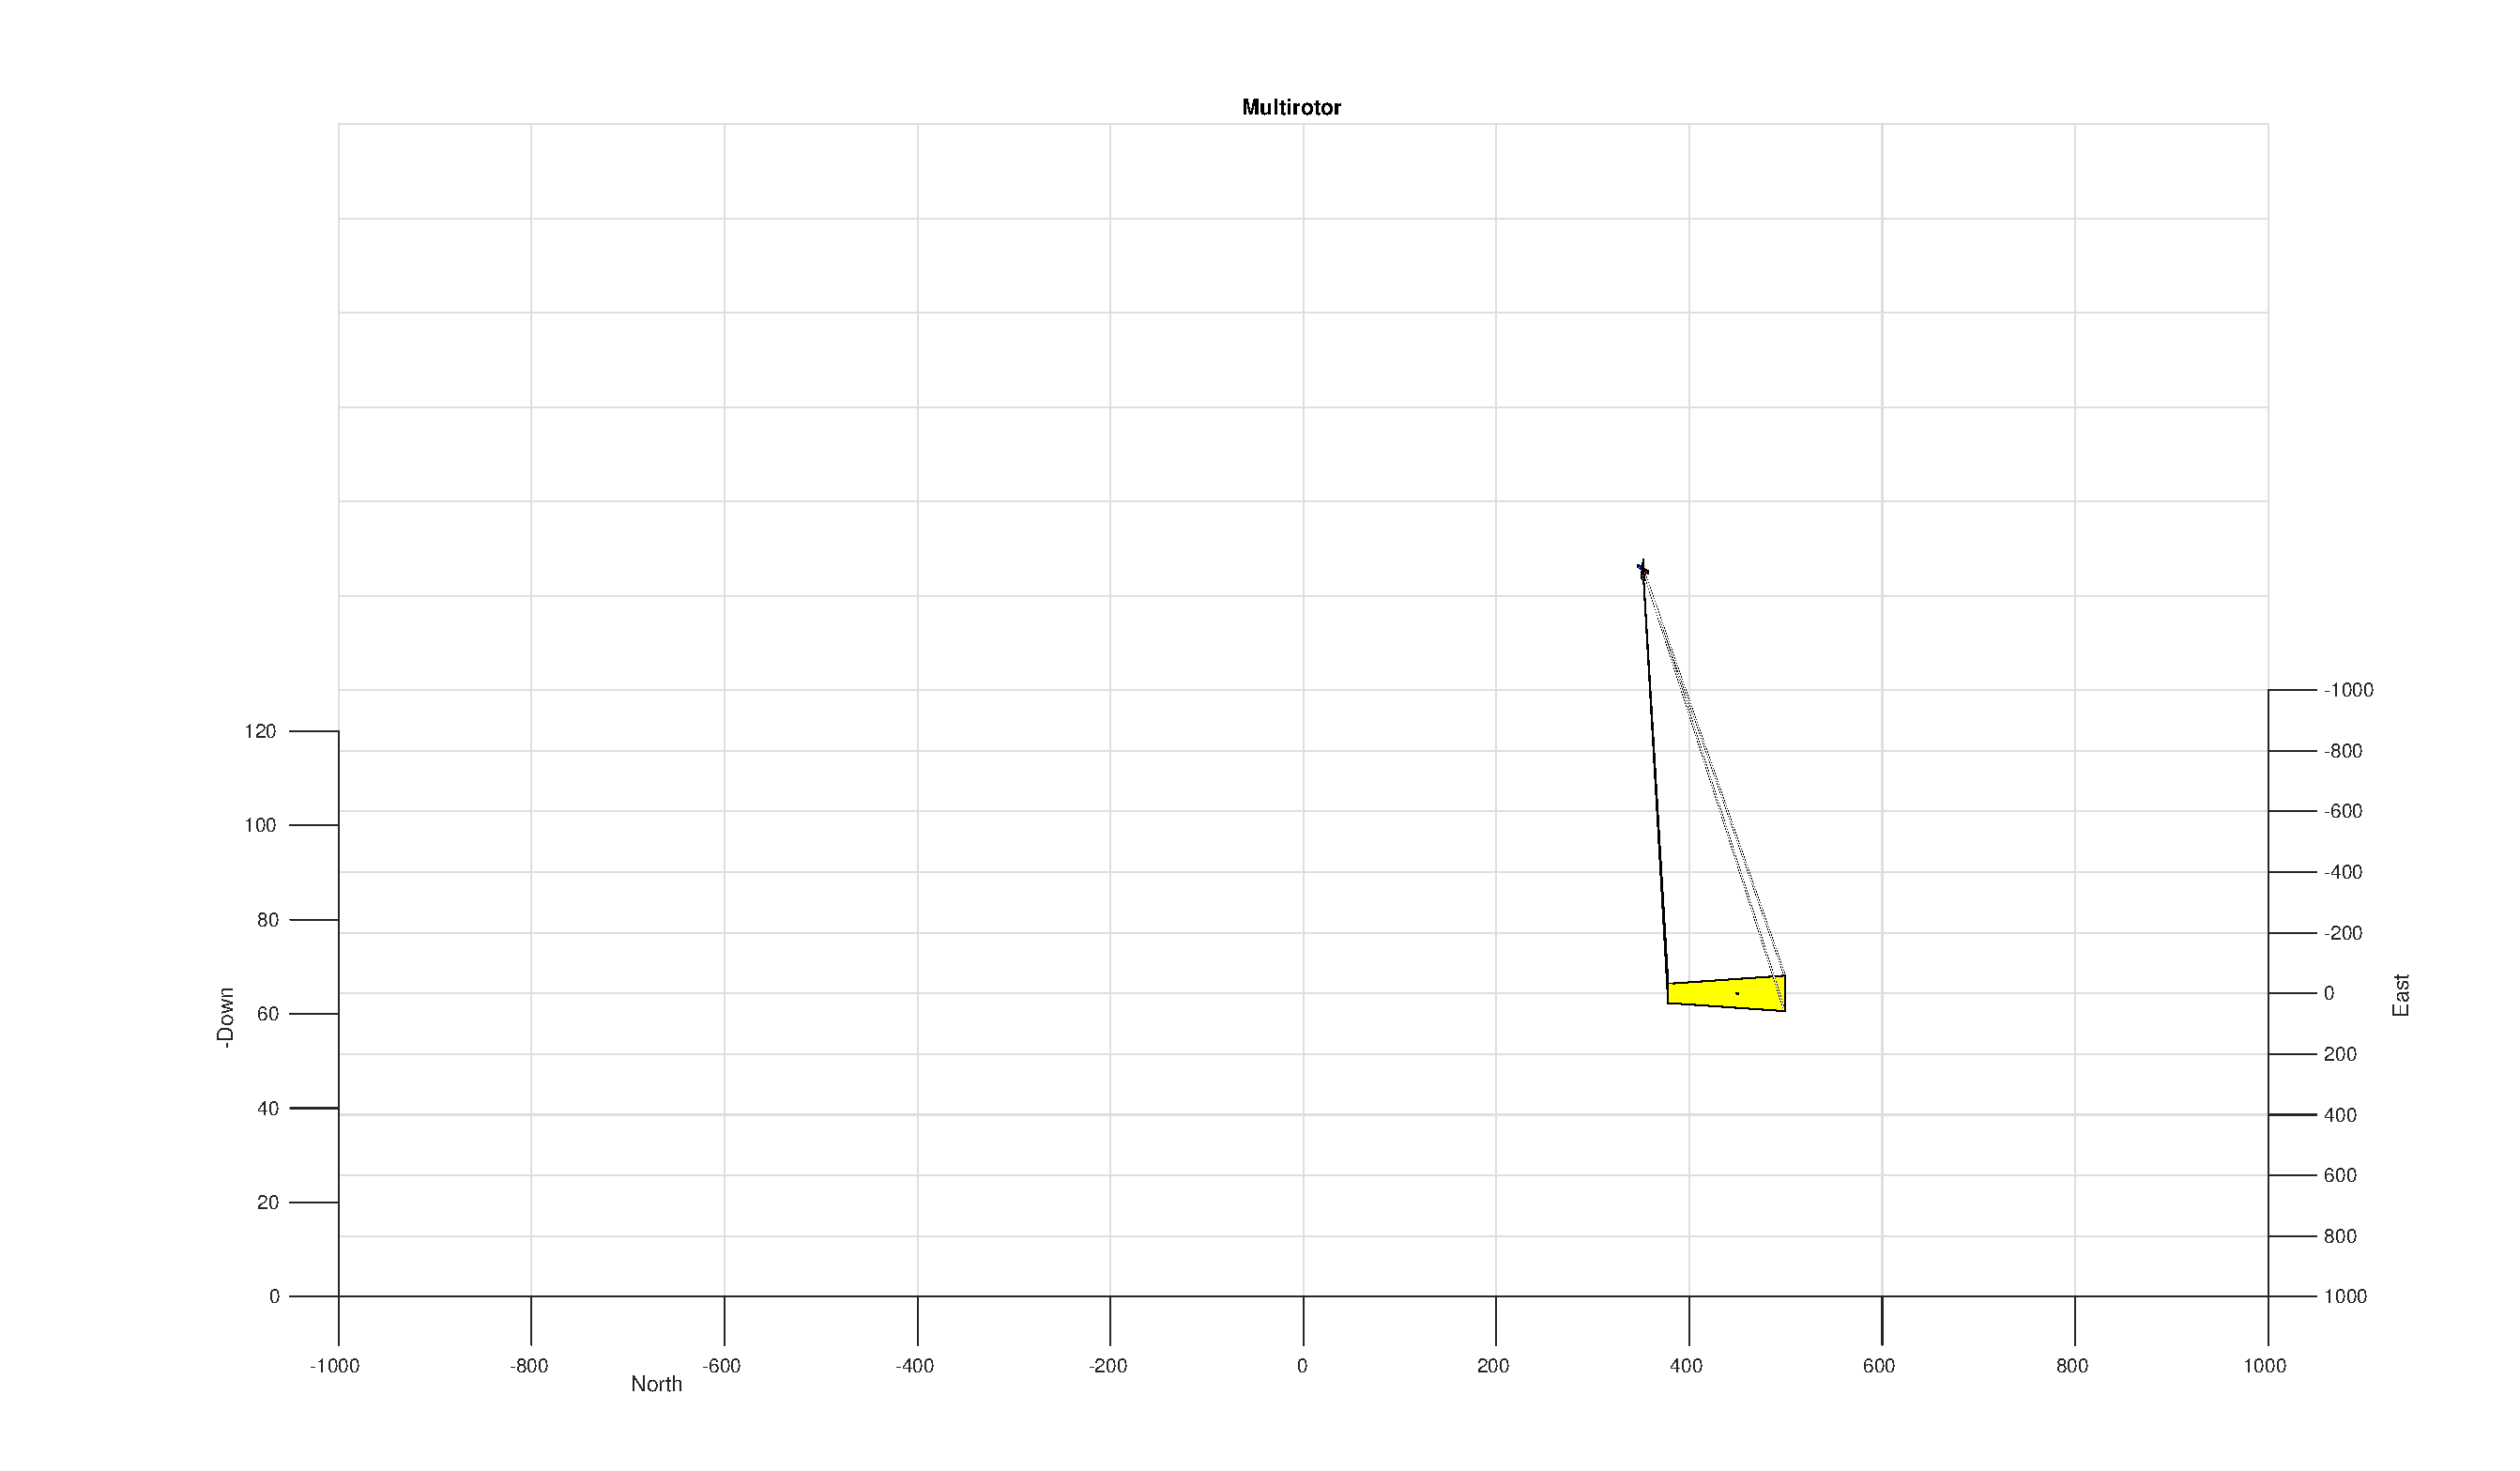
\includegraphics[width=\textwidth]{images/chapter4/inertial_UAV_5mps_90s}
		\caption{when $t=90s$}
	\end{subfigure}
	\begin{subfigure}[t]{0.32\linewidth}
		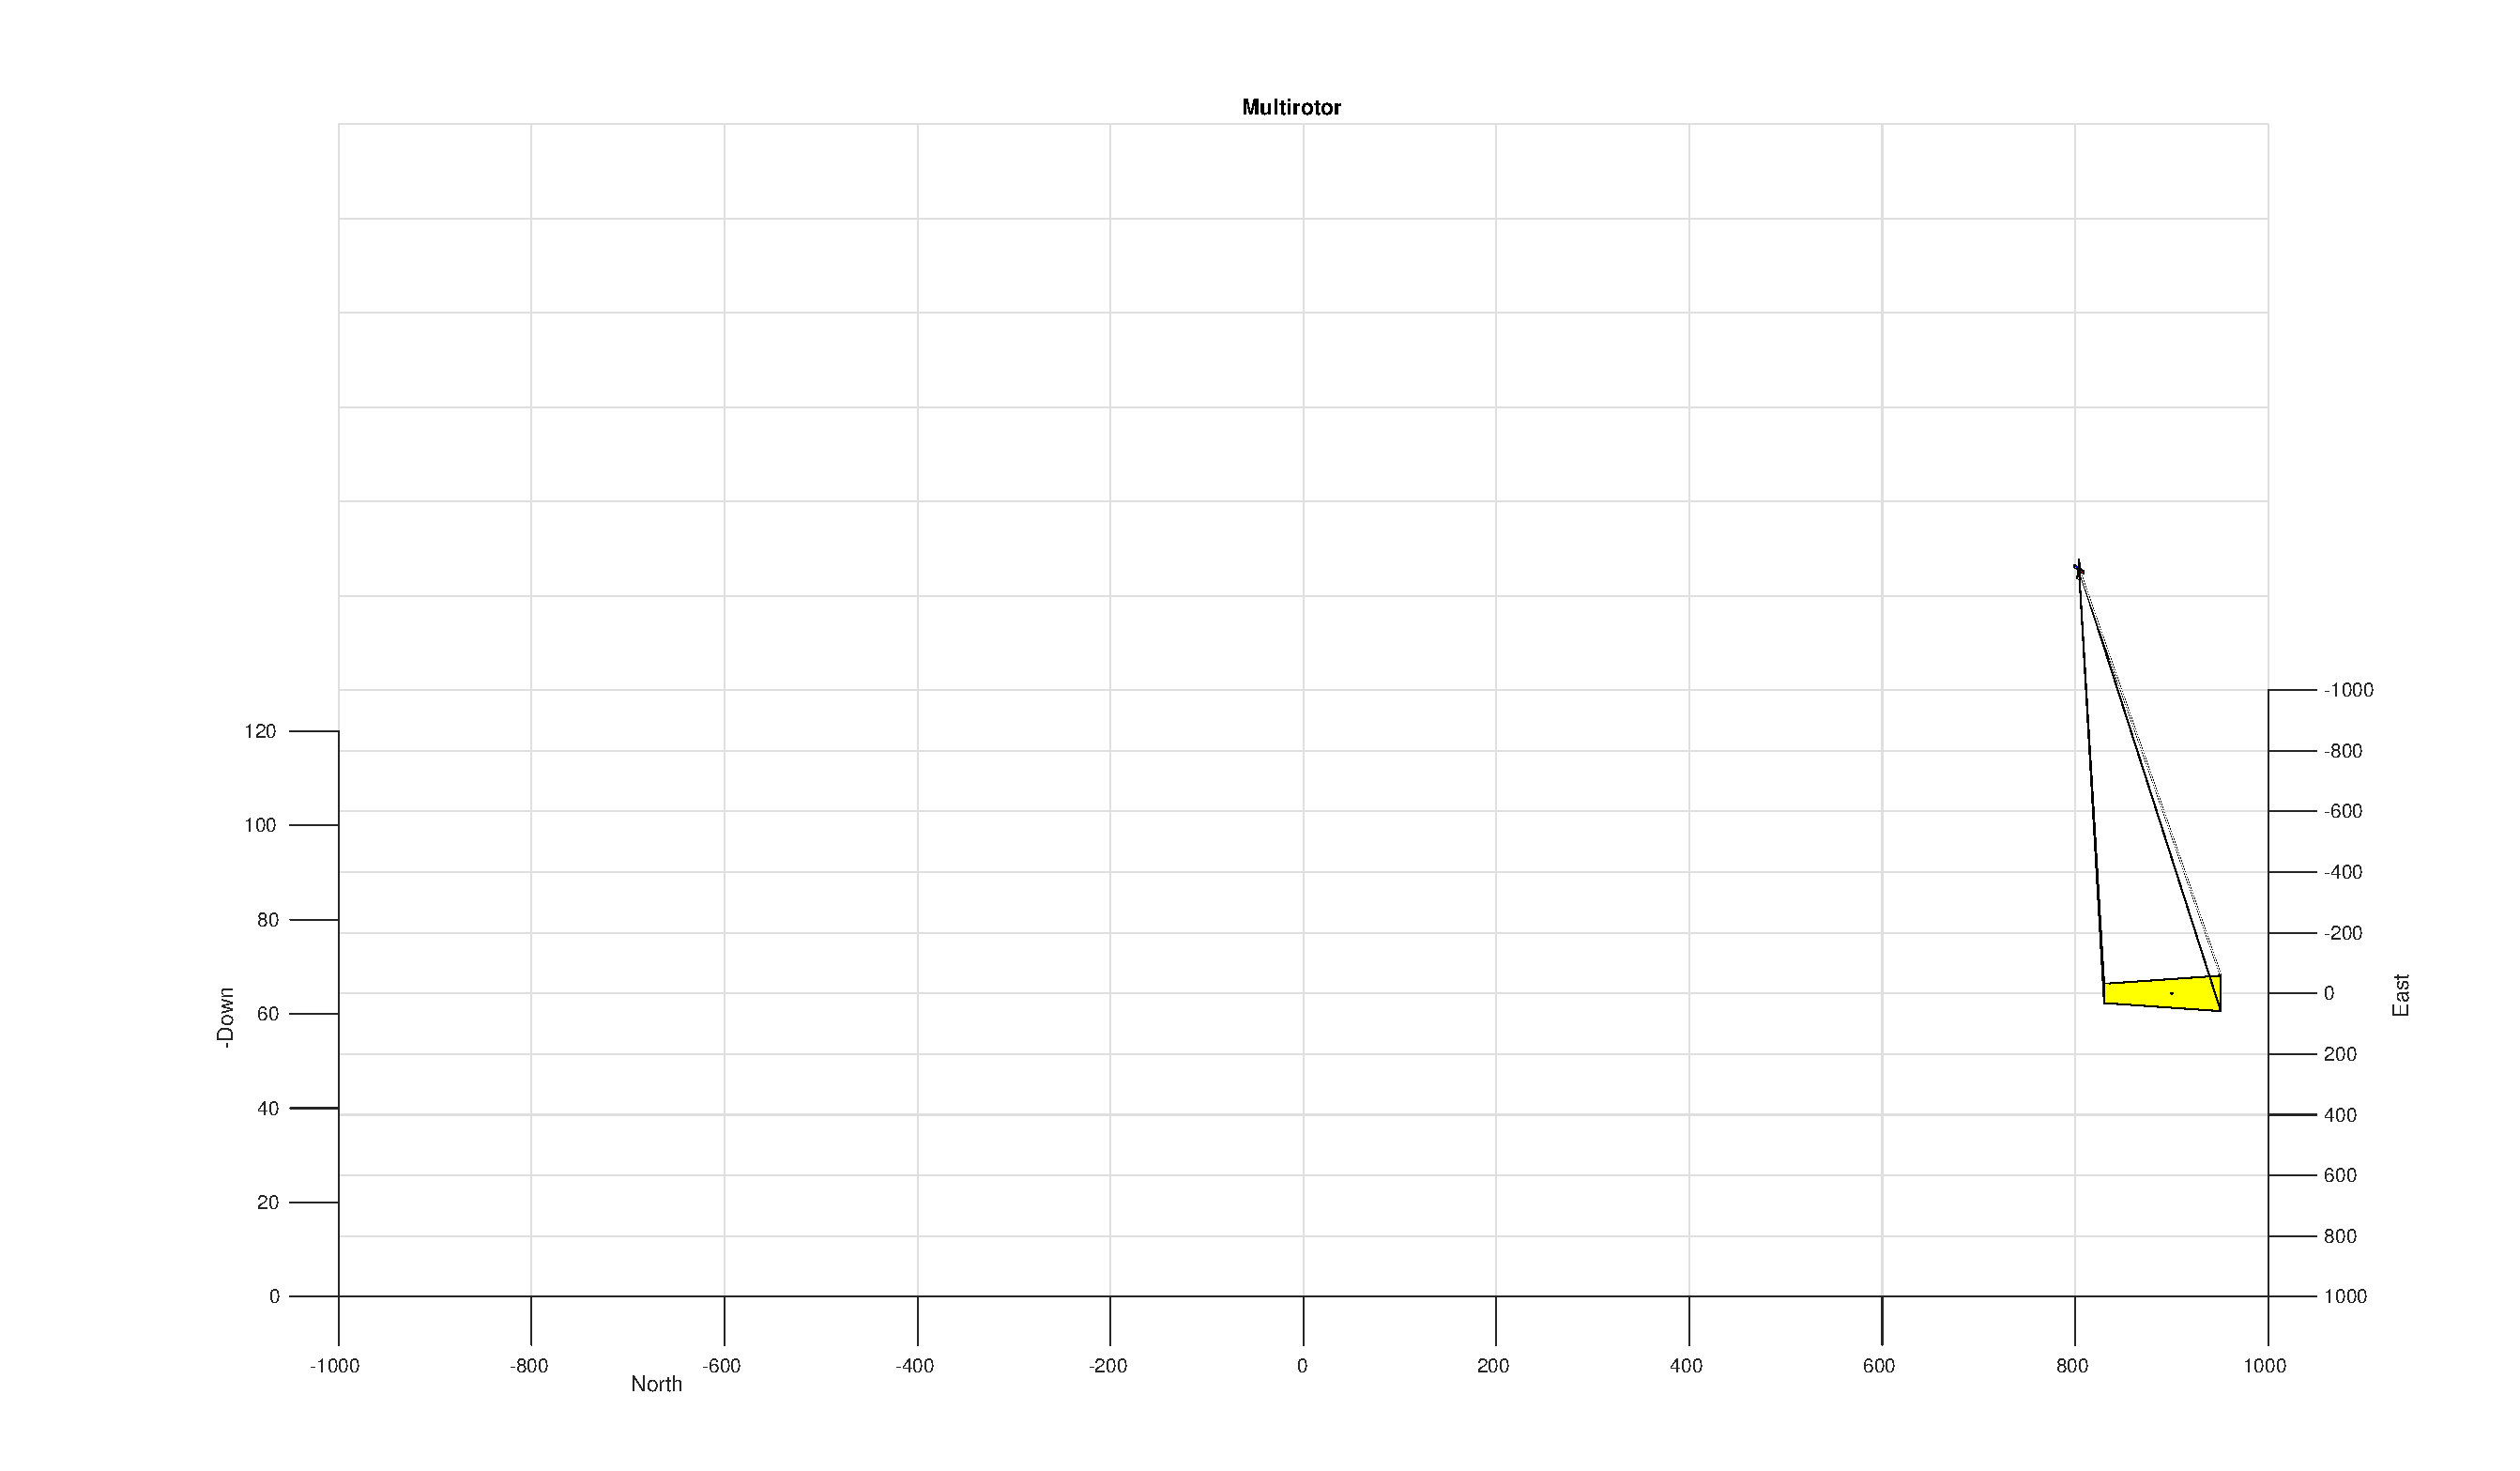
\includegraphics[width=\textwidth]{images/chapter4/inertial_UAV_5mps_180s}
		\caption{when $t=180s$}
	\end{subfigure}
	\begin{subfigure}[t]{0.32\linewidth}
		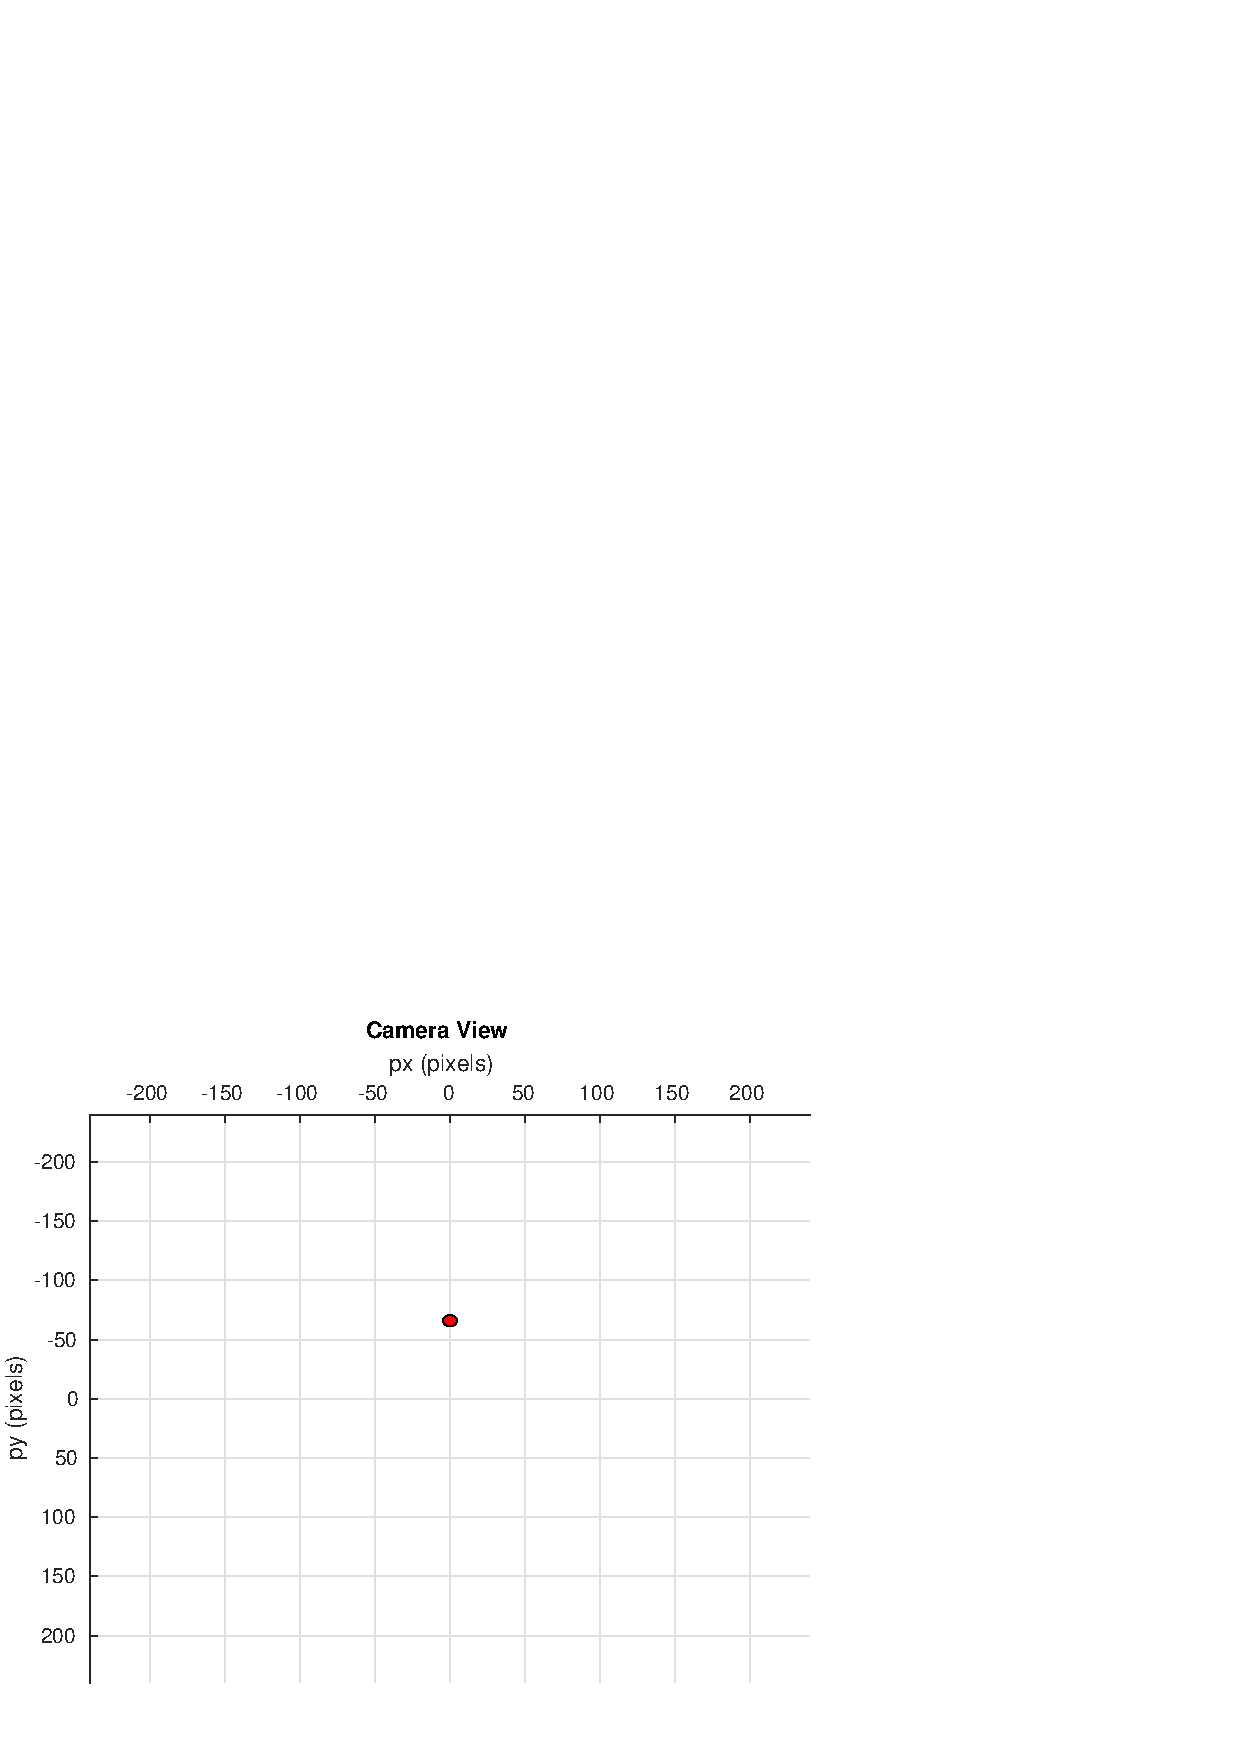
\includegraphics[width=\textwidth]{images/chapter4/inertial_camera_5mps}
		\caption{when $t=0s$}
	\end{subfigure}
	\begin{subfigure}[t]{0.32\linewidth}
		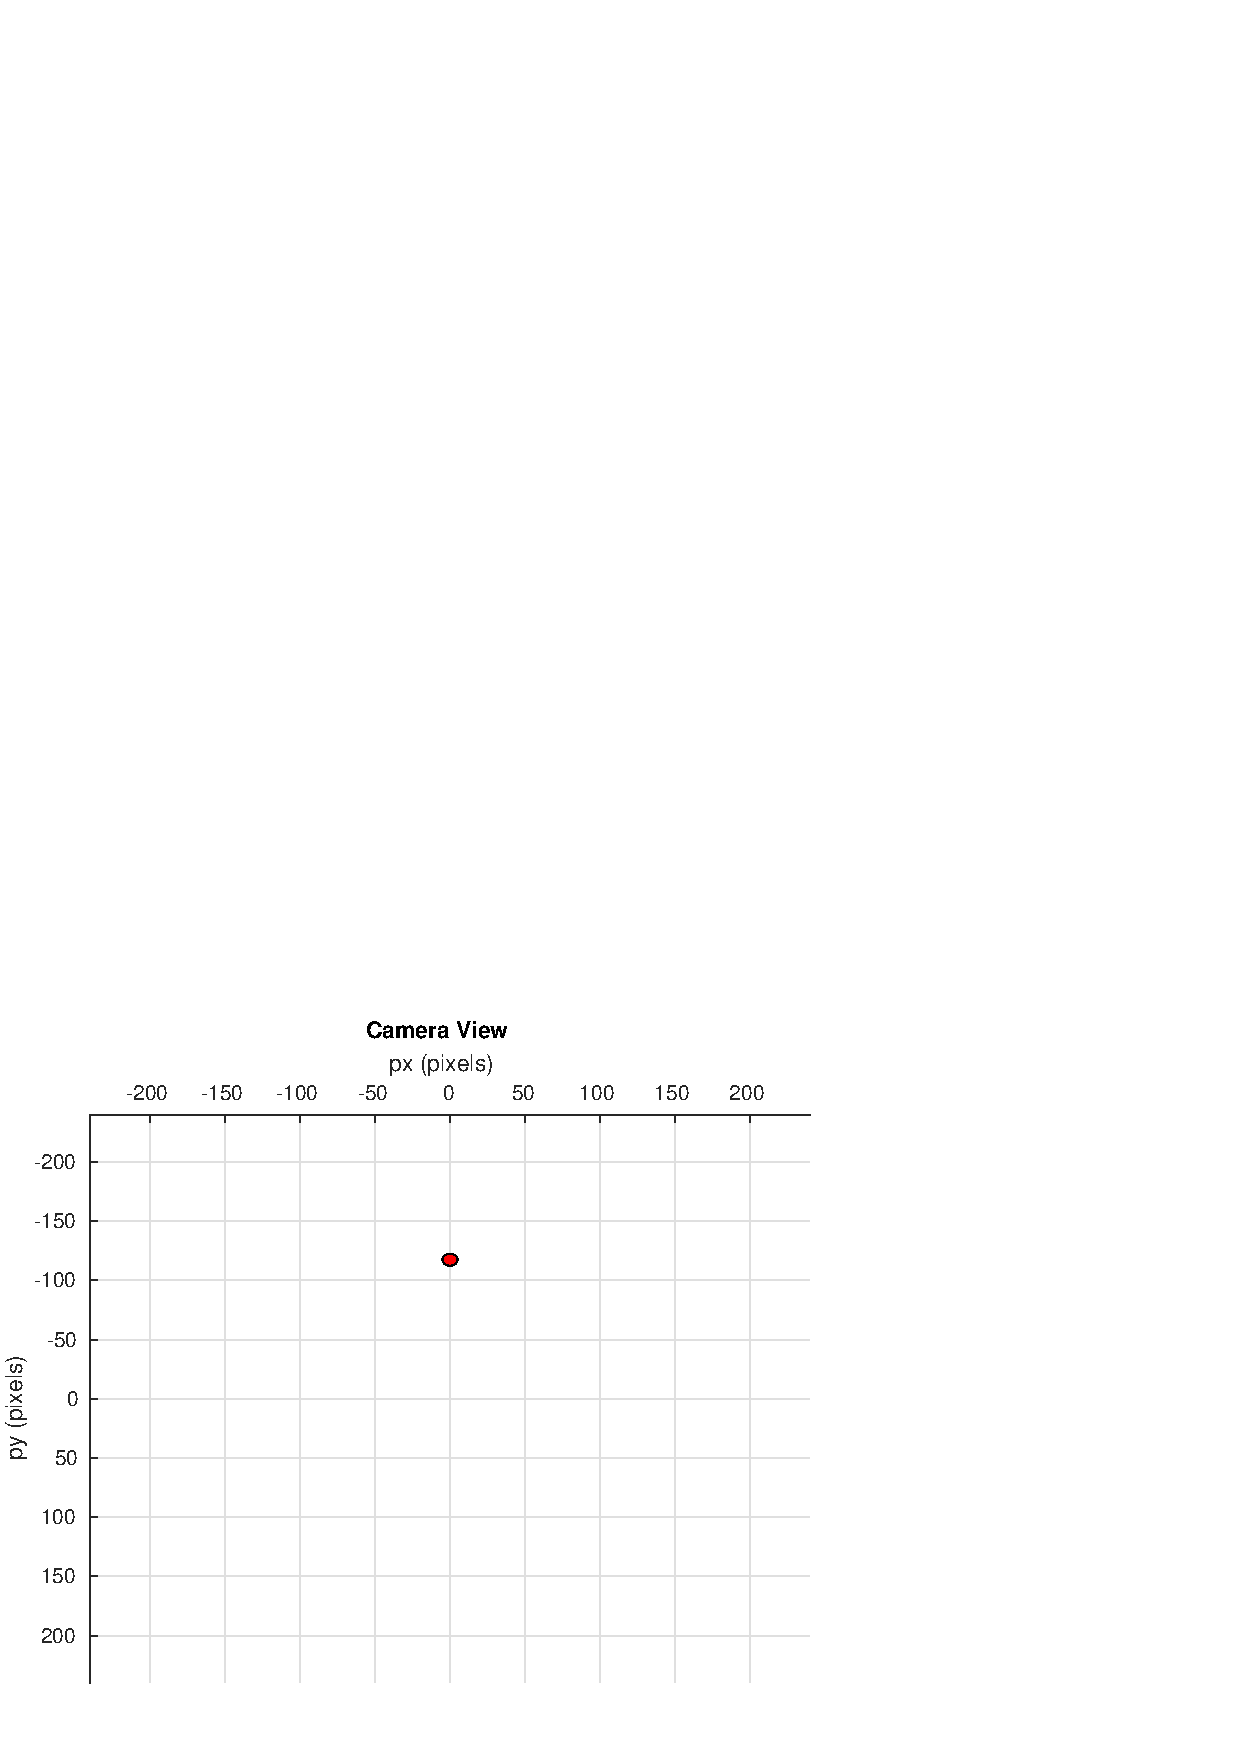
\includegraphics[width=\textwidth]{images/chapter4/inertial_camera_5mps_90s}
		\caption{when $t=90s$}
	\end{subfigure}
	\begin{subfigure}[t]{0.32\linewidth}
		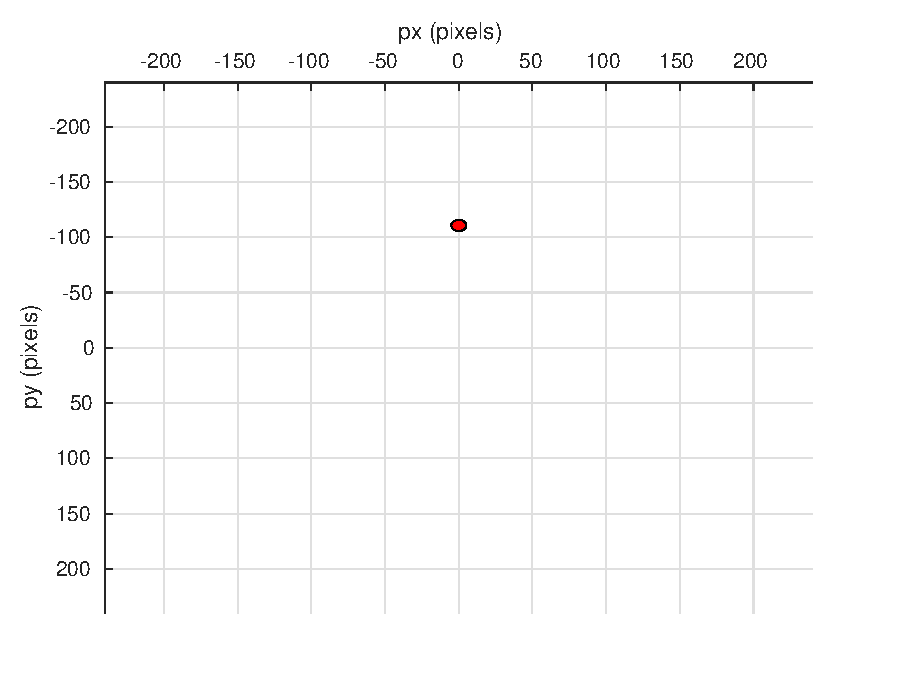
\includegraphics[width=\textwidth]{images/chapter4/inertial_camera_5mps_180s}
		\caption{when $t=180s$}
	\end{subfigure}	
	\begin{subfigure}[t]{0.8\linewidth}
		\centering
		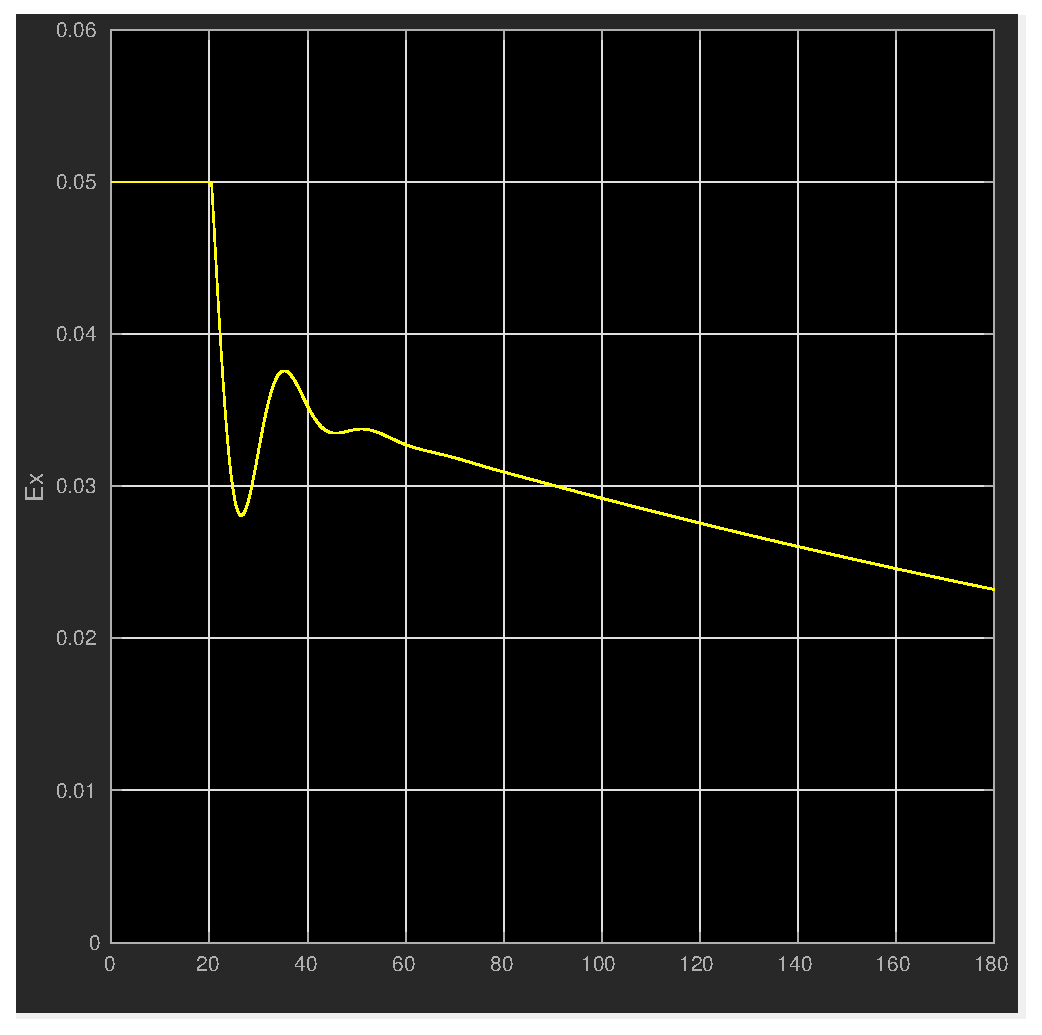
\includegraphics[width=0.5\textwidth]{images/chapter4/inertial_Ex_5mps}
		\caption{The horizontal error ($e_x$) between the unit LOS vector and the unit optical axis vector both in the vehicle-1 frame converges to zero. It saturates at 0.05 to prevent the multirotor from commanding too large torque command.}
	\end{subfigure}	
	\caption{Simulation result for the backstepping control using the inertial LOS vector. The ground target is moving at the speed of $5m/s$. The initial UAV and target positions are [-110, 0, -90] and [0, 0, 0] respectively. Tuning parameters are set to $k=0.12$, $k_1=1$, $k_2=1$, $k_3=1$, and $\Gamma=0.01*I_3$ (identity matrix). In this case, the target is not placed at the center of image because the horizontal error is computed in the vehicle-1 frame meaning that the pitch of multirotor is not compensated.}
	\label{inertial_5mps}
\end{figure}

\begin{figure}[htbp]
	\centering
	\begin{subfigure}[t]{0.32\linewidth}
		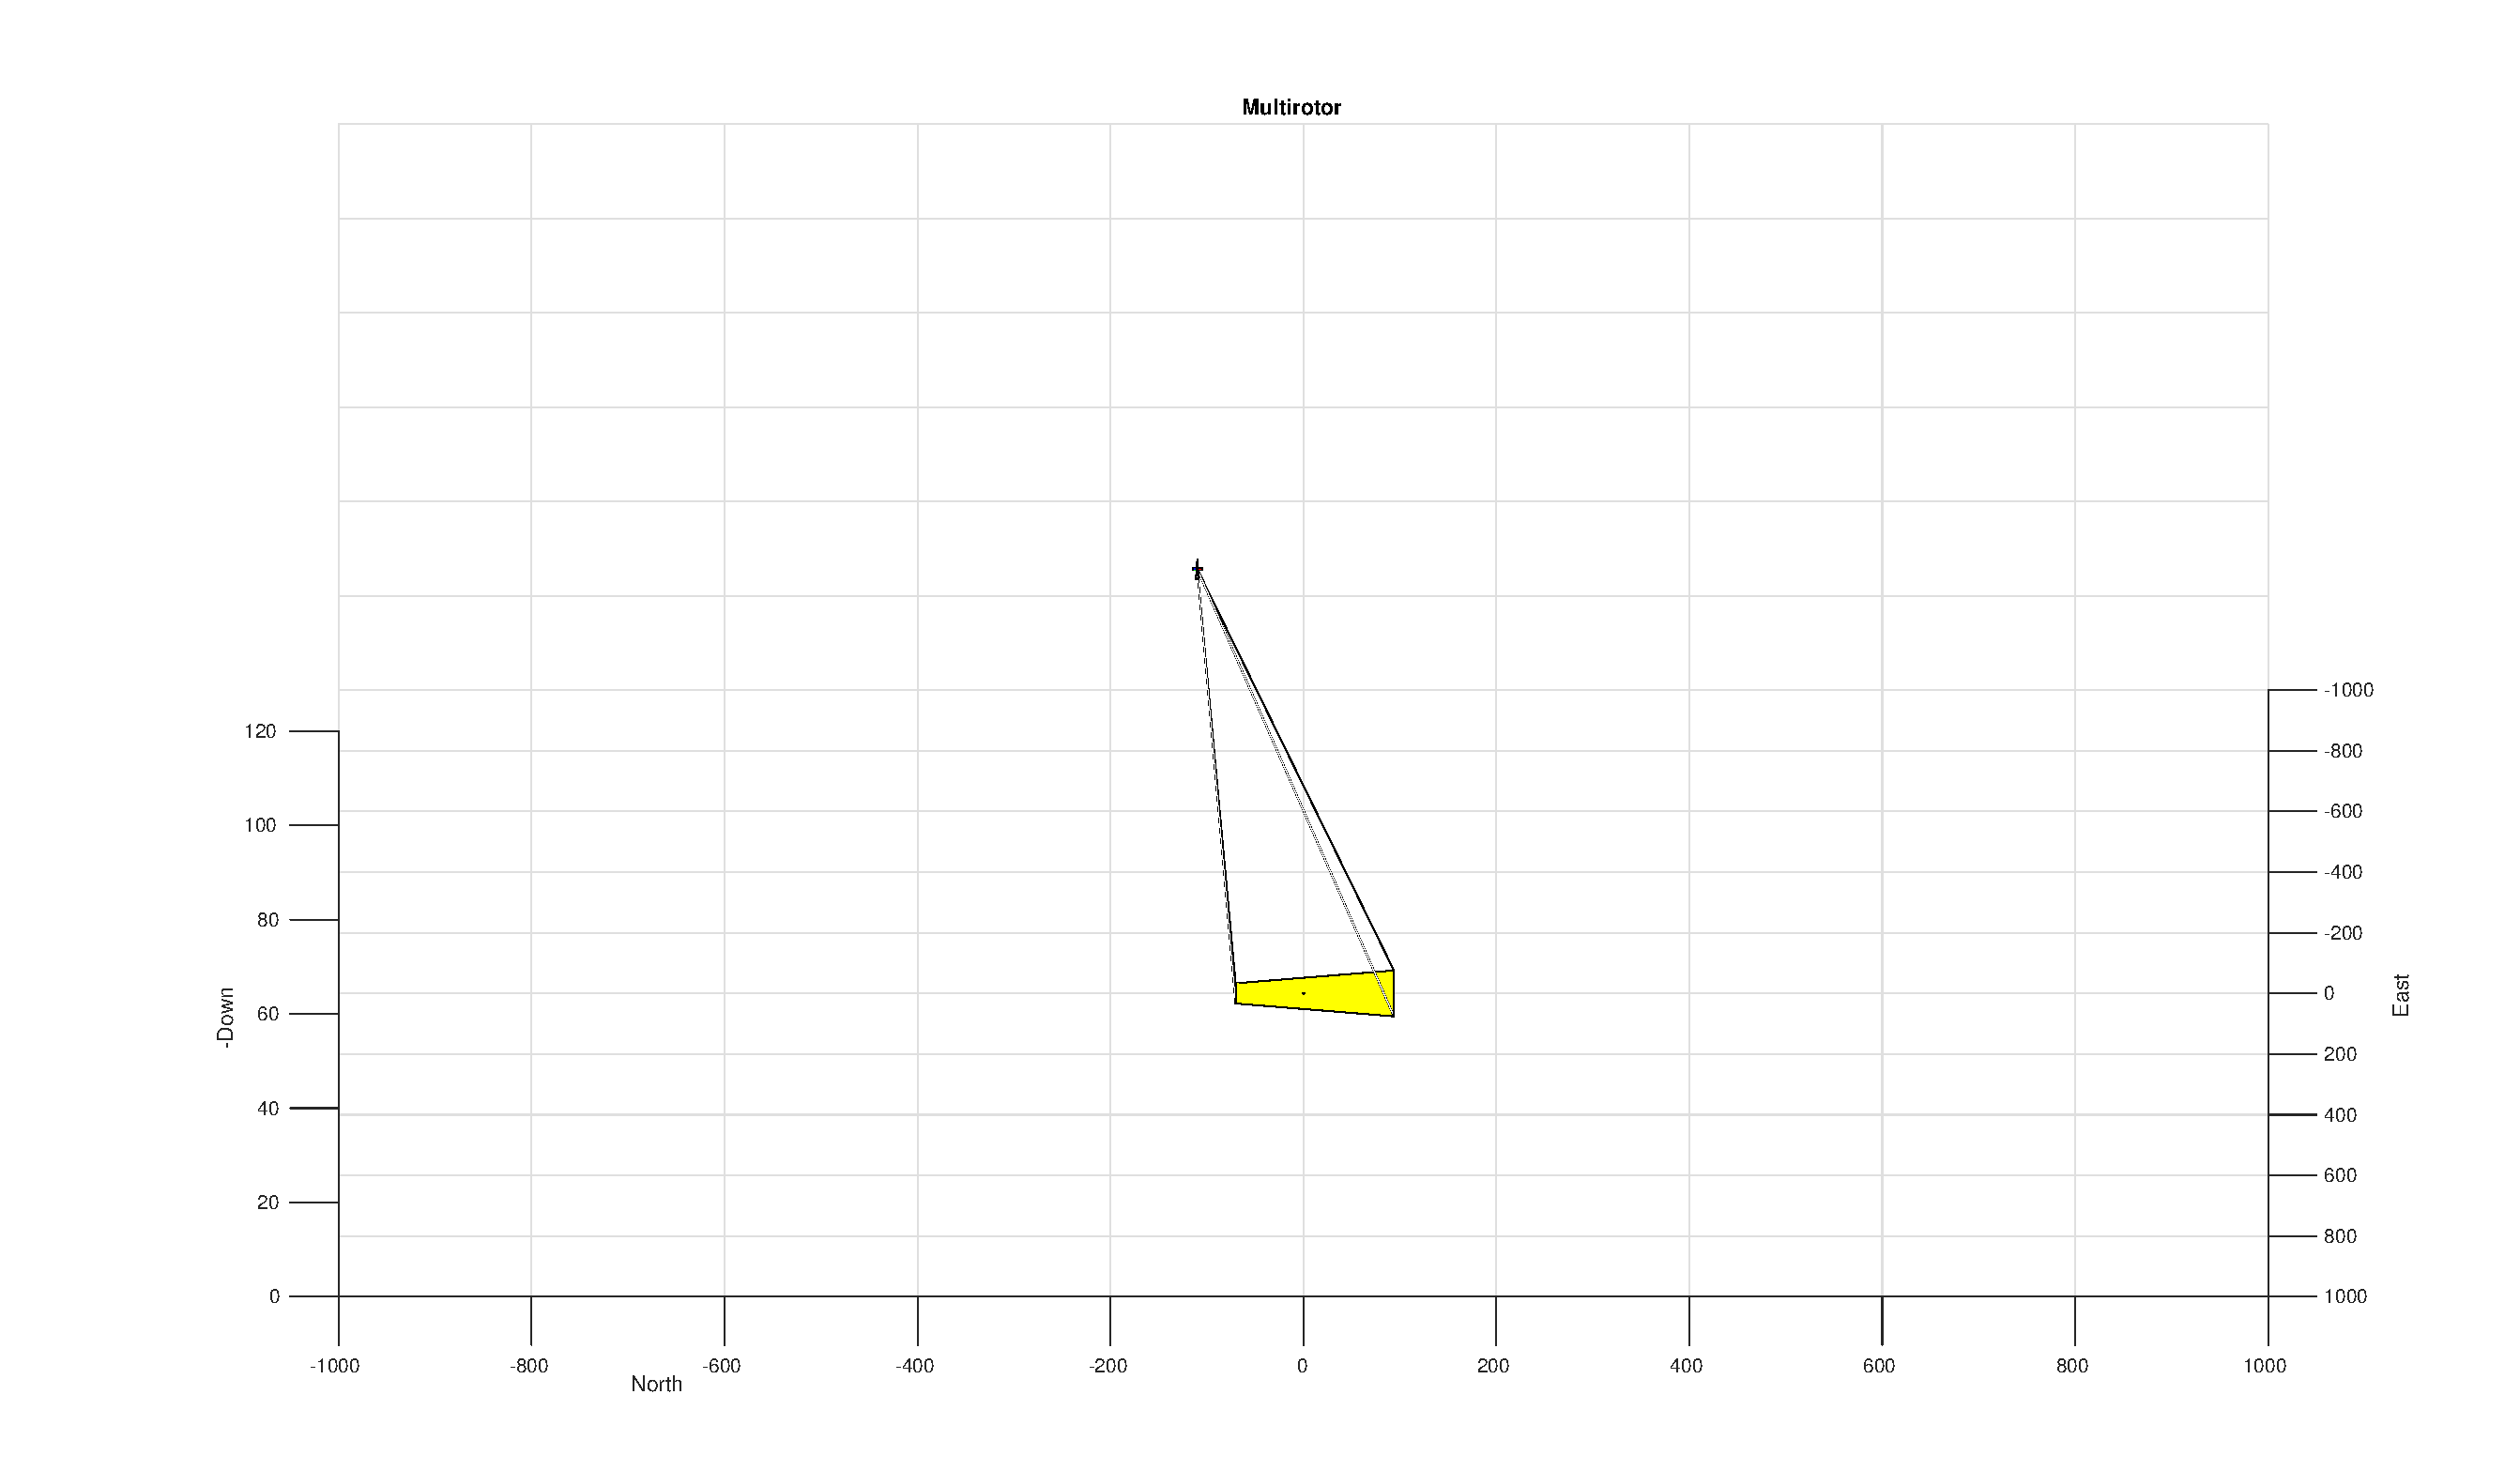
\includegraphics[width=\textwidth]{images/chapter4/inertial_UAV_-5mps}
		\caption{when $t=0s$}
	\end{subfigure}
	\begin{subfigure}[t]{0.32\linewidth}
		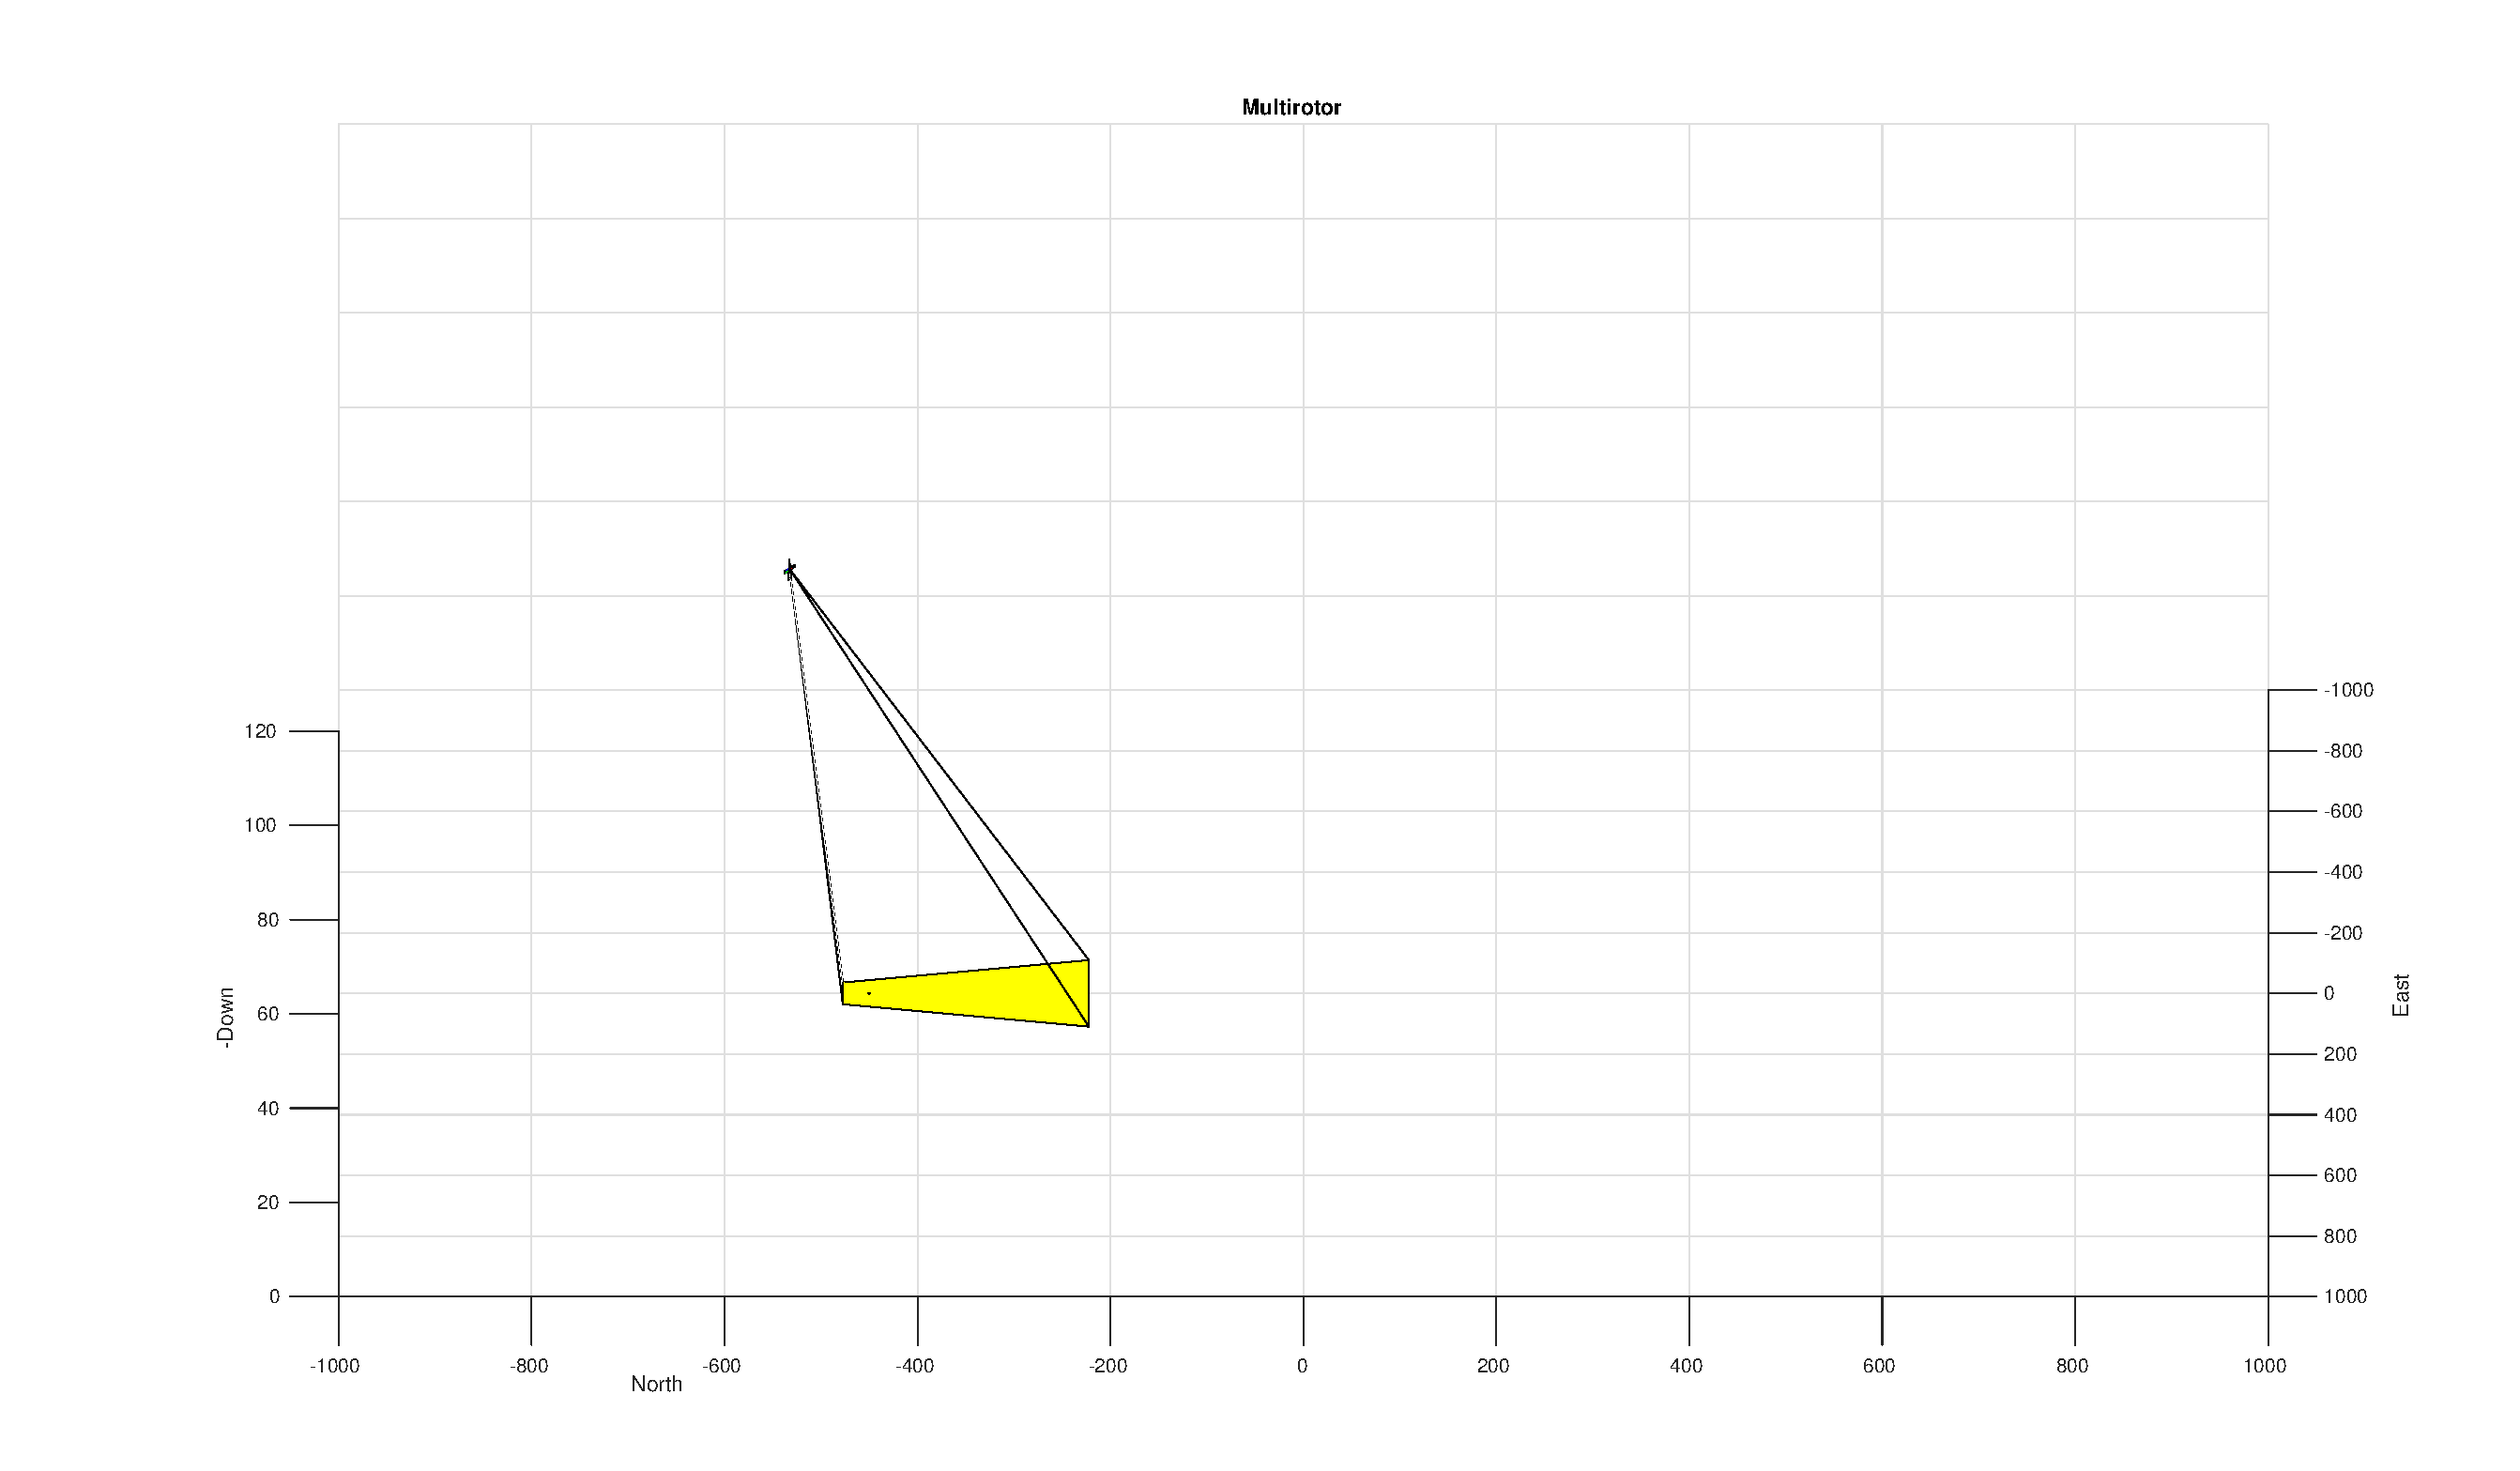
\includegraphics[width=\textwidth]{images/chapter4/inertial_UAV_-5mps_90s}
		\caption{when $t=90s$}
	\end{subfigure}
	\begin{subfigure}[t]{0.32\linewidth}
		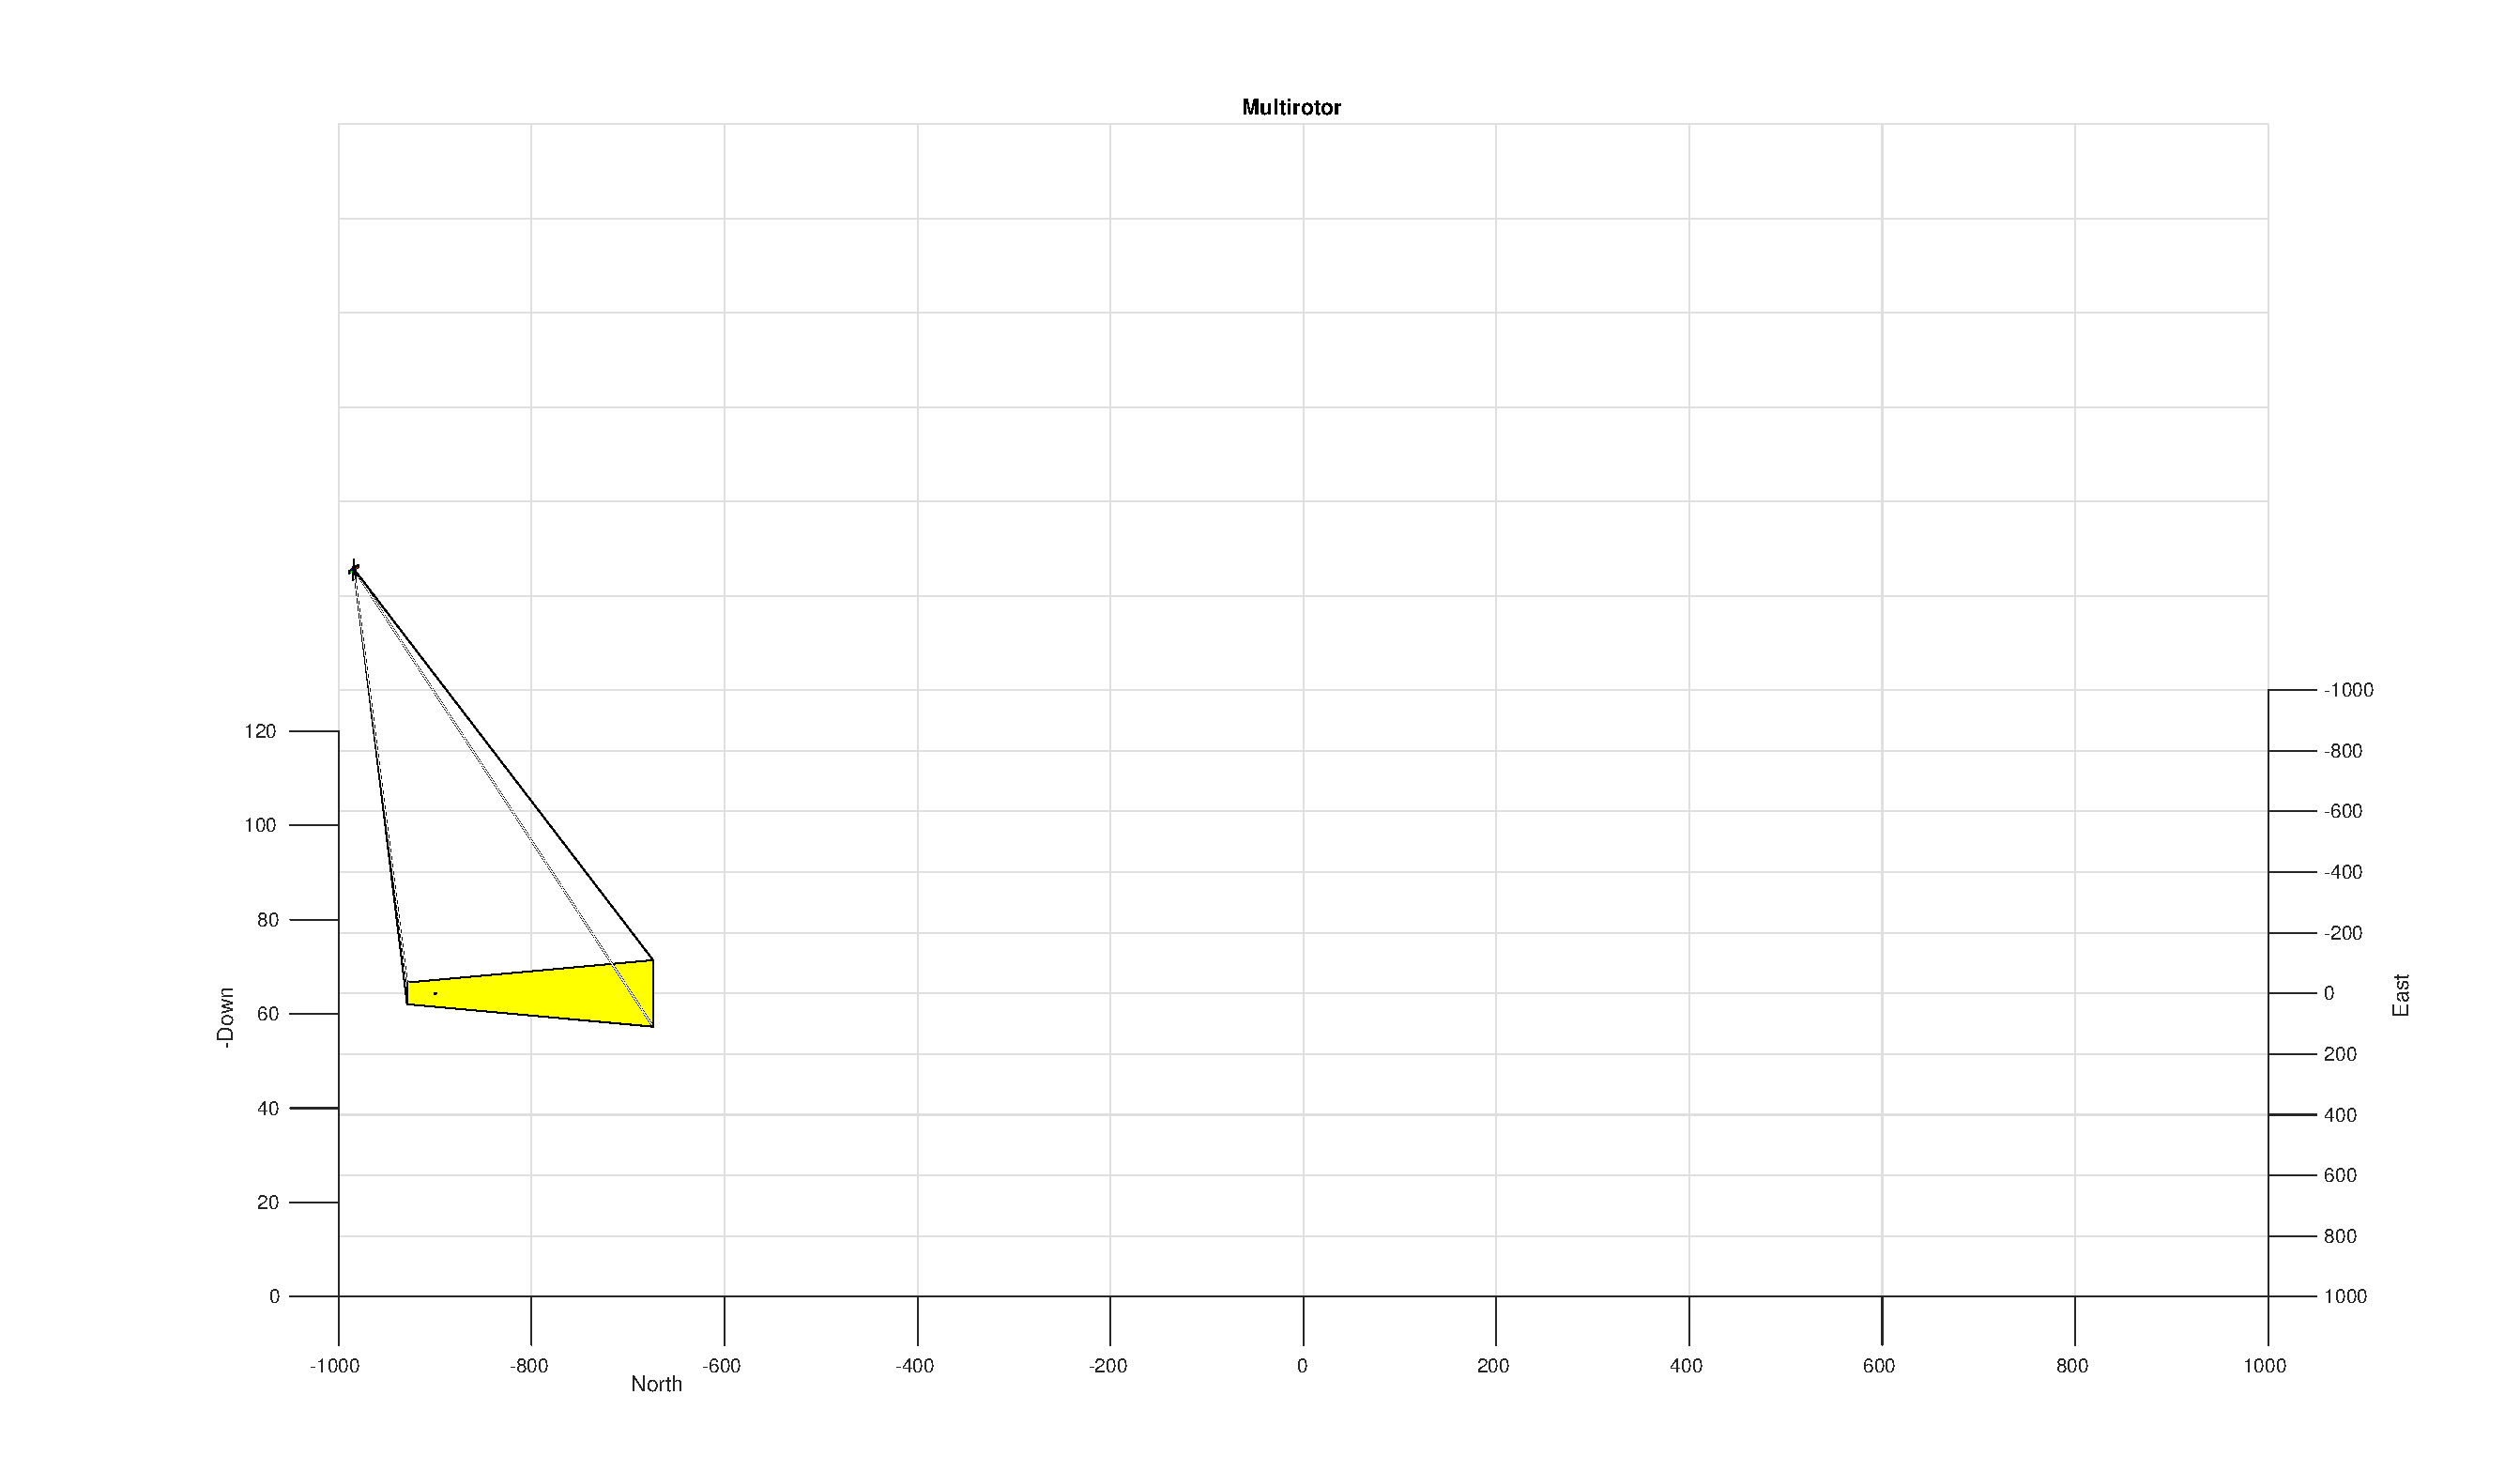
\includegraphics[width=\textwidth]{images/chapter4/inertial_UAV_-5mps_180s}
		\caption{when $t=180s$}
	\end{subfigure}
	\begin{subfigure}[t]{0.32\linewidth}
		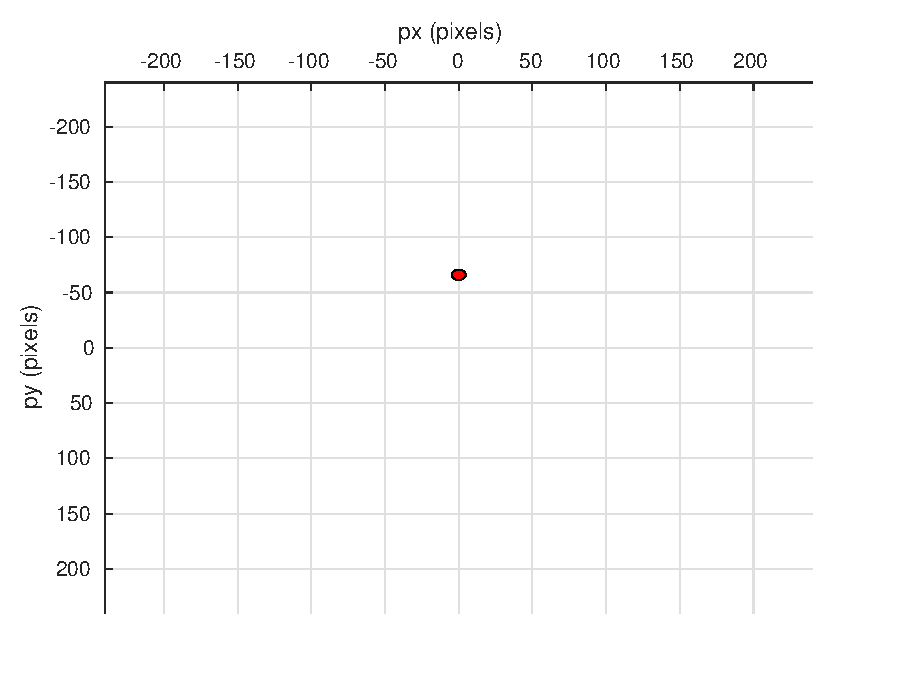
\includegraphics[width=\textwidth]{images/chapter4/inertial_camera_-5mps}
		\caption{when $t=0s$}
	\end{subfigure}
	\begin{subfigure}[t]{0.32\linewidth}
		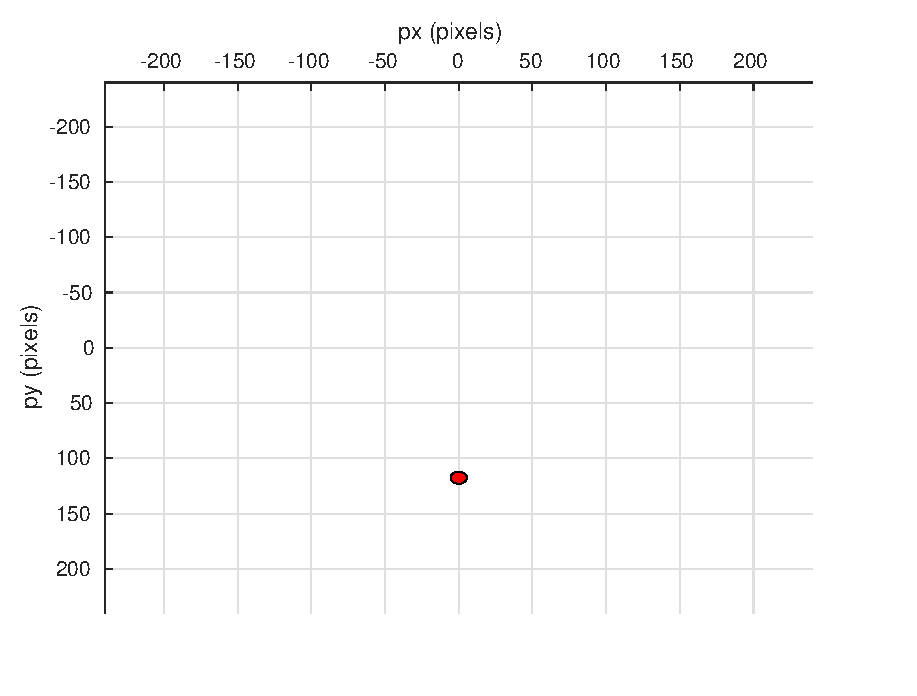
\includegraphics[width=\textwidth]{images/chapter4/inertial_camera_-5mps_90s}
		\caption{when $t=90s$}
	\end{subfigure}
	\begin{subfigure}[t]{0.32\linewidth}
		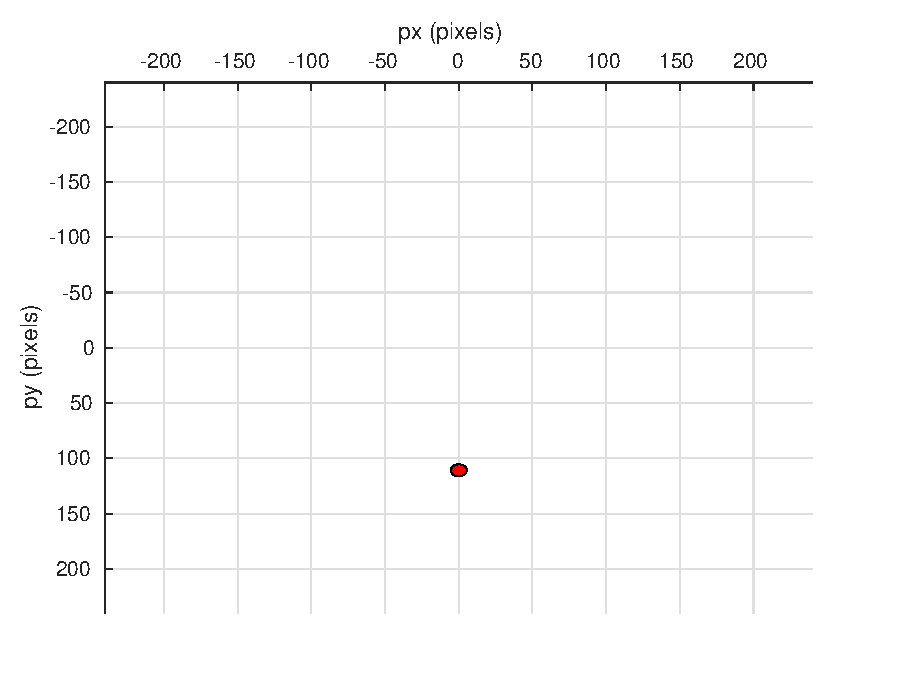
\includegraphics[width=\textwidth]{images/chapter4/inertial_camera_-5mps_180s}
		\caption{when $t=180s$}
	\end{subfigure}	
	\begin{subfigure}[t]{0.8\linewidth}
		\centering
		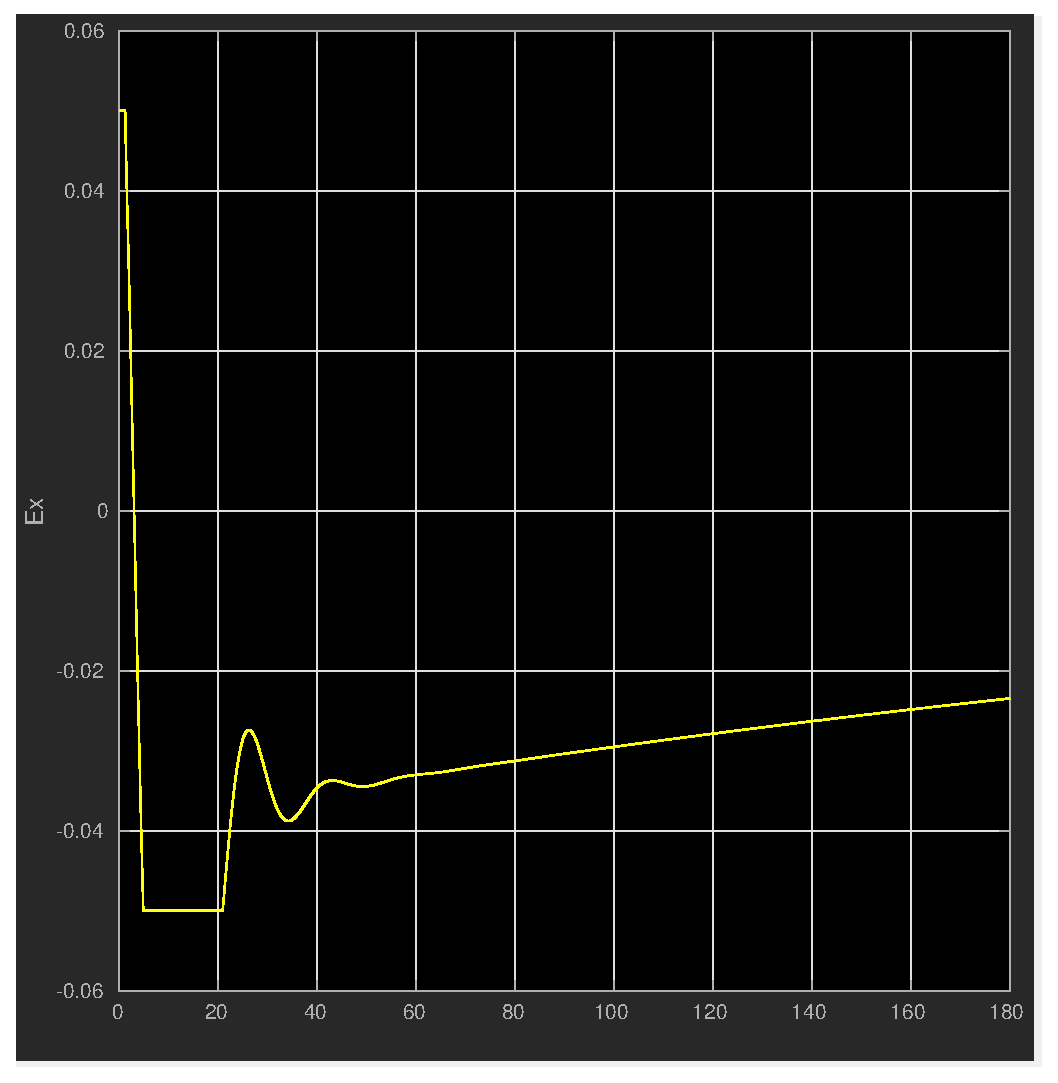
\includegraphics[width=0.5\textwidth]{images/chapter4/inertial_Ex_-5mps}
		\caption{The horizontal error ($e_x$) between the unit LOS vector and the unit optical axis vector both in the vehicle-1 frame converges to zero. It saturates at 0.05 to prevent the multirotor from commanding too large torque command.}
	\end{subfigure}	
	\caption{Simulation result for the backstepping control using the inertial LOS vector. The ground target is moving at the speed of $-5m/s$. The initial UAV and target positions are [-110, 0, -90] and [0, 0, 0] respectively. Tuning parameters are set to $k=0.12$, $k_1=1$, $k_2=1$, $k_3=1$, and $\Gamma=0.01*I_3$ (identity matrix). In this case, the target is not placed at the center of image because the horizontal error is computed in the vehicle-1 frame meaning that the pitch of multirotor is not compensated.}
	\label{inertial_-5mps}
\end{figure}

The second backstepping controller is the actual simulation of the hardware demonstration. When the multirotor is equipped with monocular camera only, the multirotor has no other way to know where the target is relative to itself but through the information received from the camera. Thus, the second controller is only using the camera information (target pixel location) to control the multirotor (See Figure \ref{system_image}). The camera is simulated to output its information at $30Hz$ while the backstepping controller is evaluated at $100Hz$. This caused the horizontal error $e_x$ to be quite noisy which eventually makes the controller unstable. Thus, a low-pass filter is added to smooth $e_x$. The simulation results for a static target, moving targets at $5m/s$ and $-5m/s$ can be found in Figure \ref{image_0mps}, \ref{image_5mps}, and \ref{image_-5mps} respectively. It turns out that there is no significant performance decrease using the sparse image information compared to using the inertial LOS vector directly. 

\begin{figure}[htbp]
	\centering
	\begin{subfigure}[t]{0.45\linewidth}
		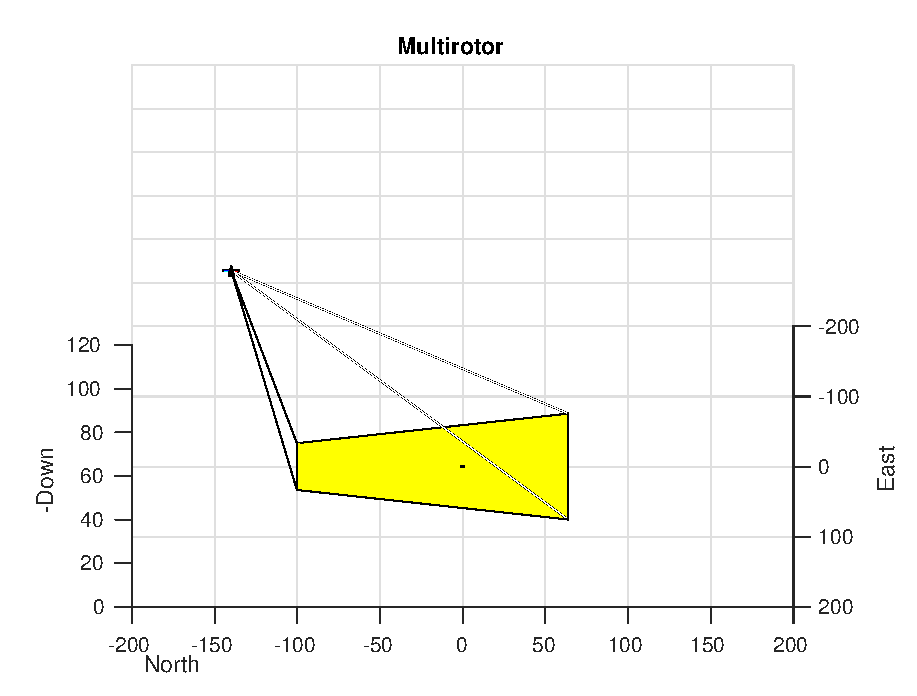
\includegraphics[width=\textwidth]{images/chapter4/image_UAV_0mps}
		\caption{Multirotor and ground target when $t=0s$}
	\end{subfigure}
	\begin{subfigure}[t]{0.45\linewidth}
		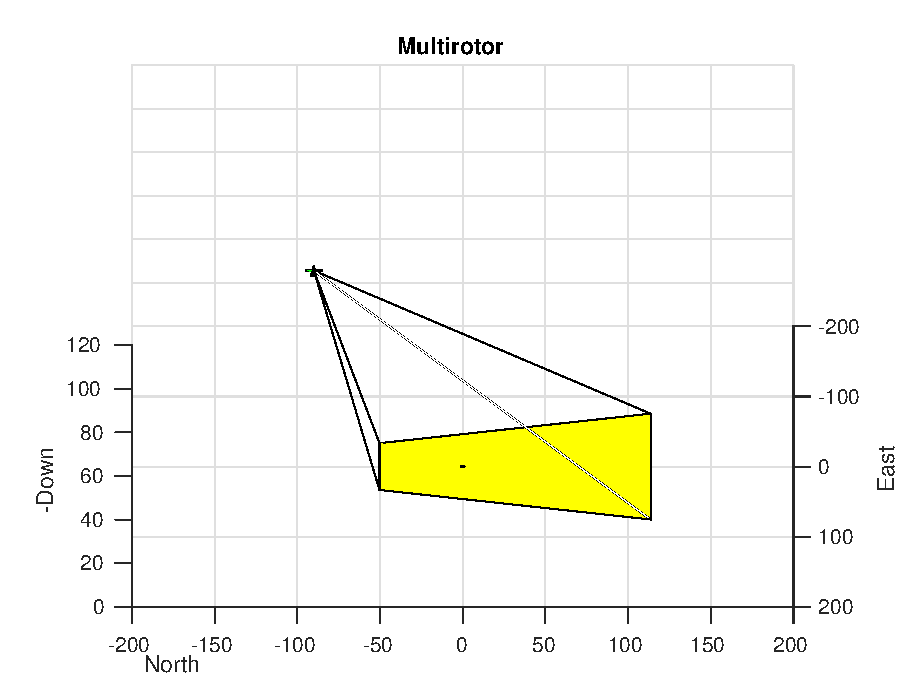
\includegraphics[width=\textwidth]{images/chapter4/image_UAV_0mps_60s}
		\caption{when $t=60s$}
	\end{subfigure}
	\begin{subfigure}[t]{0.45\linewidth}
		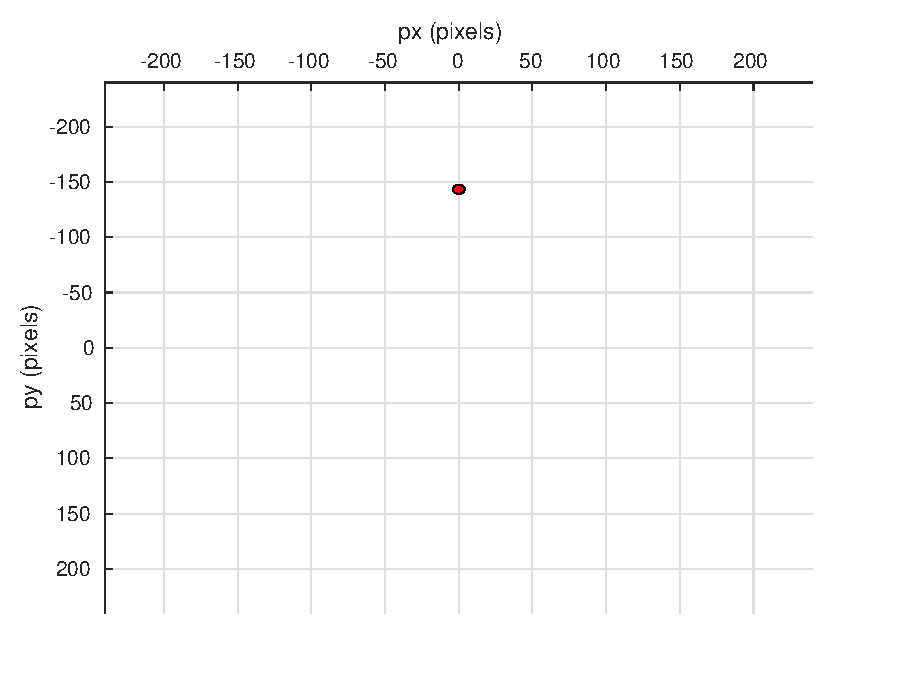
\includegraphics[width=\textwidth]{images/chapter4/image_camera_0mps}
		\caption{Camera view when $t=0s$}
	\end{subfigure}
	\begin{subfigure}[t]{0.45\linewidth}
		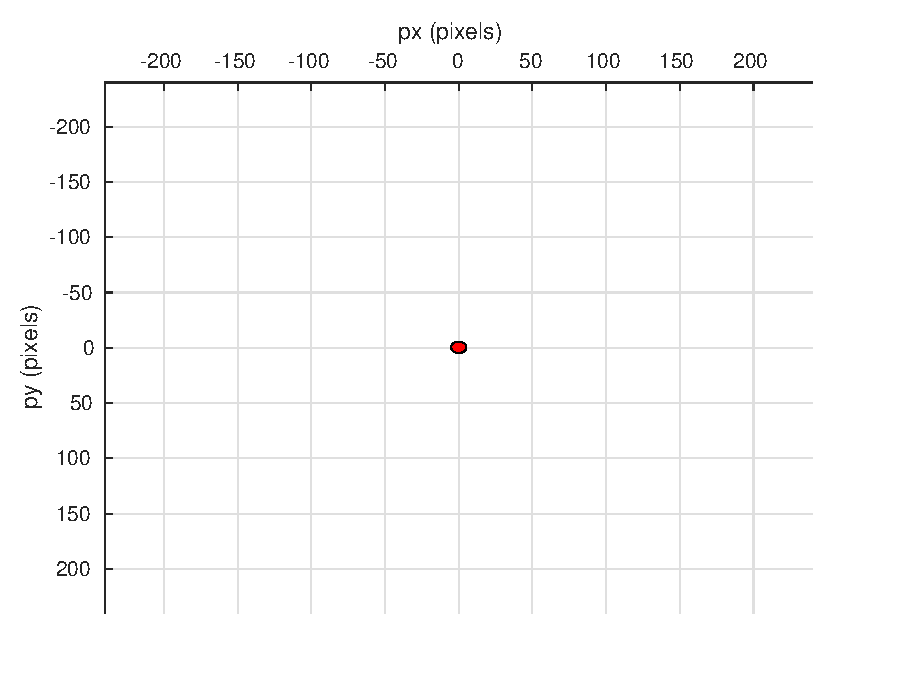
\includegraphics[width=\textwidth]{images/chapter4/image_camera_0mps_60s}
		\caption{when $t=60s$}
	\end{subfigure}
	\begin{subfigure}[t]{0.8\linewidth}
		\centering
		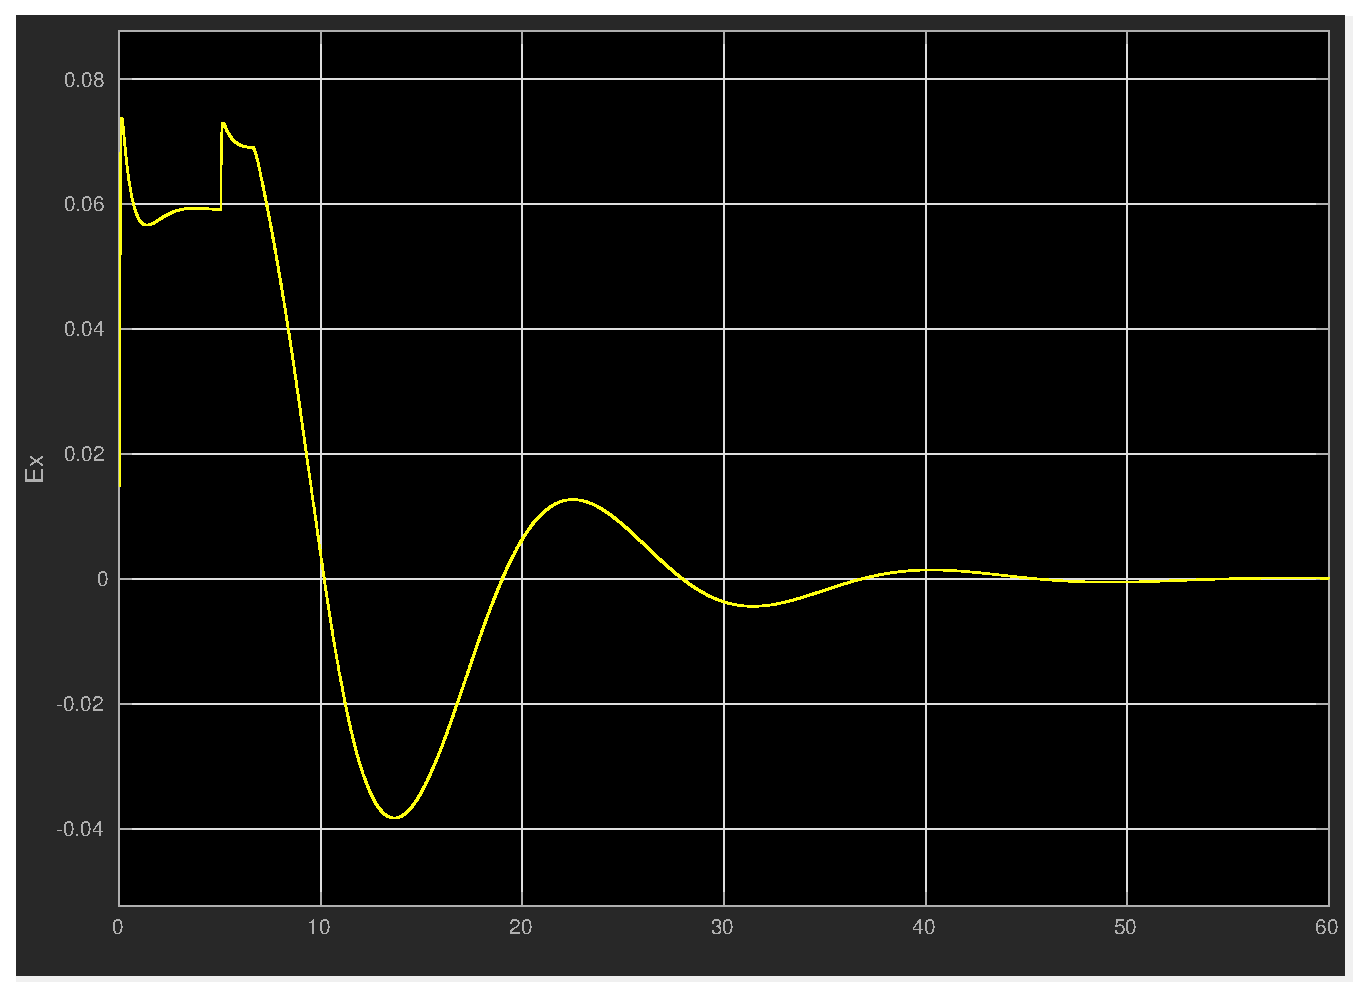
\includegraphics[width=0.5\textwidth]{images/chapter4/image_Ex_0mps}
		\caption{The horizontal error ($e_x$) between the normalized target pixel coordinates and the unit optical axis vector both in the vehicle-1 frame converges to zero. Note that the value is low-pass filtered.}
	\end{subfigure}	
	\caption{Simulation result for the backstepping control using the normalized target pixel coordinates. The ground target is static ($0m/s$). The initial UAV and target positions are [-140, 0, -90] and [0, 0, 0] respectively. Tuning parameters are set to $k=0.12$, $k_1=1$, $k_2=1$, $k_3=1$, and $\Gamma=0.01*I_3$ (identity matrix).}
	\label{image_0mps}
\end{figure}

\begin{figure}[htbp]
	\centering
	\begin{subfigure}[t]{0.32\linewidth}
		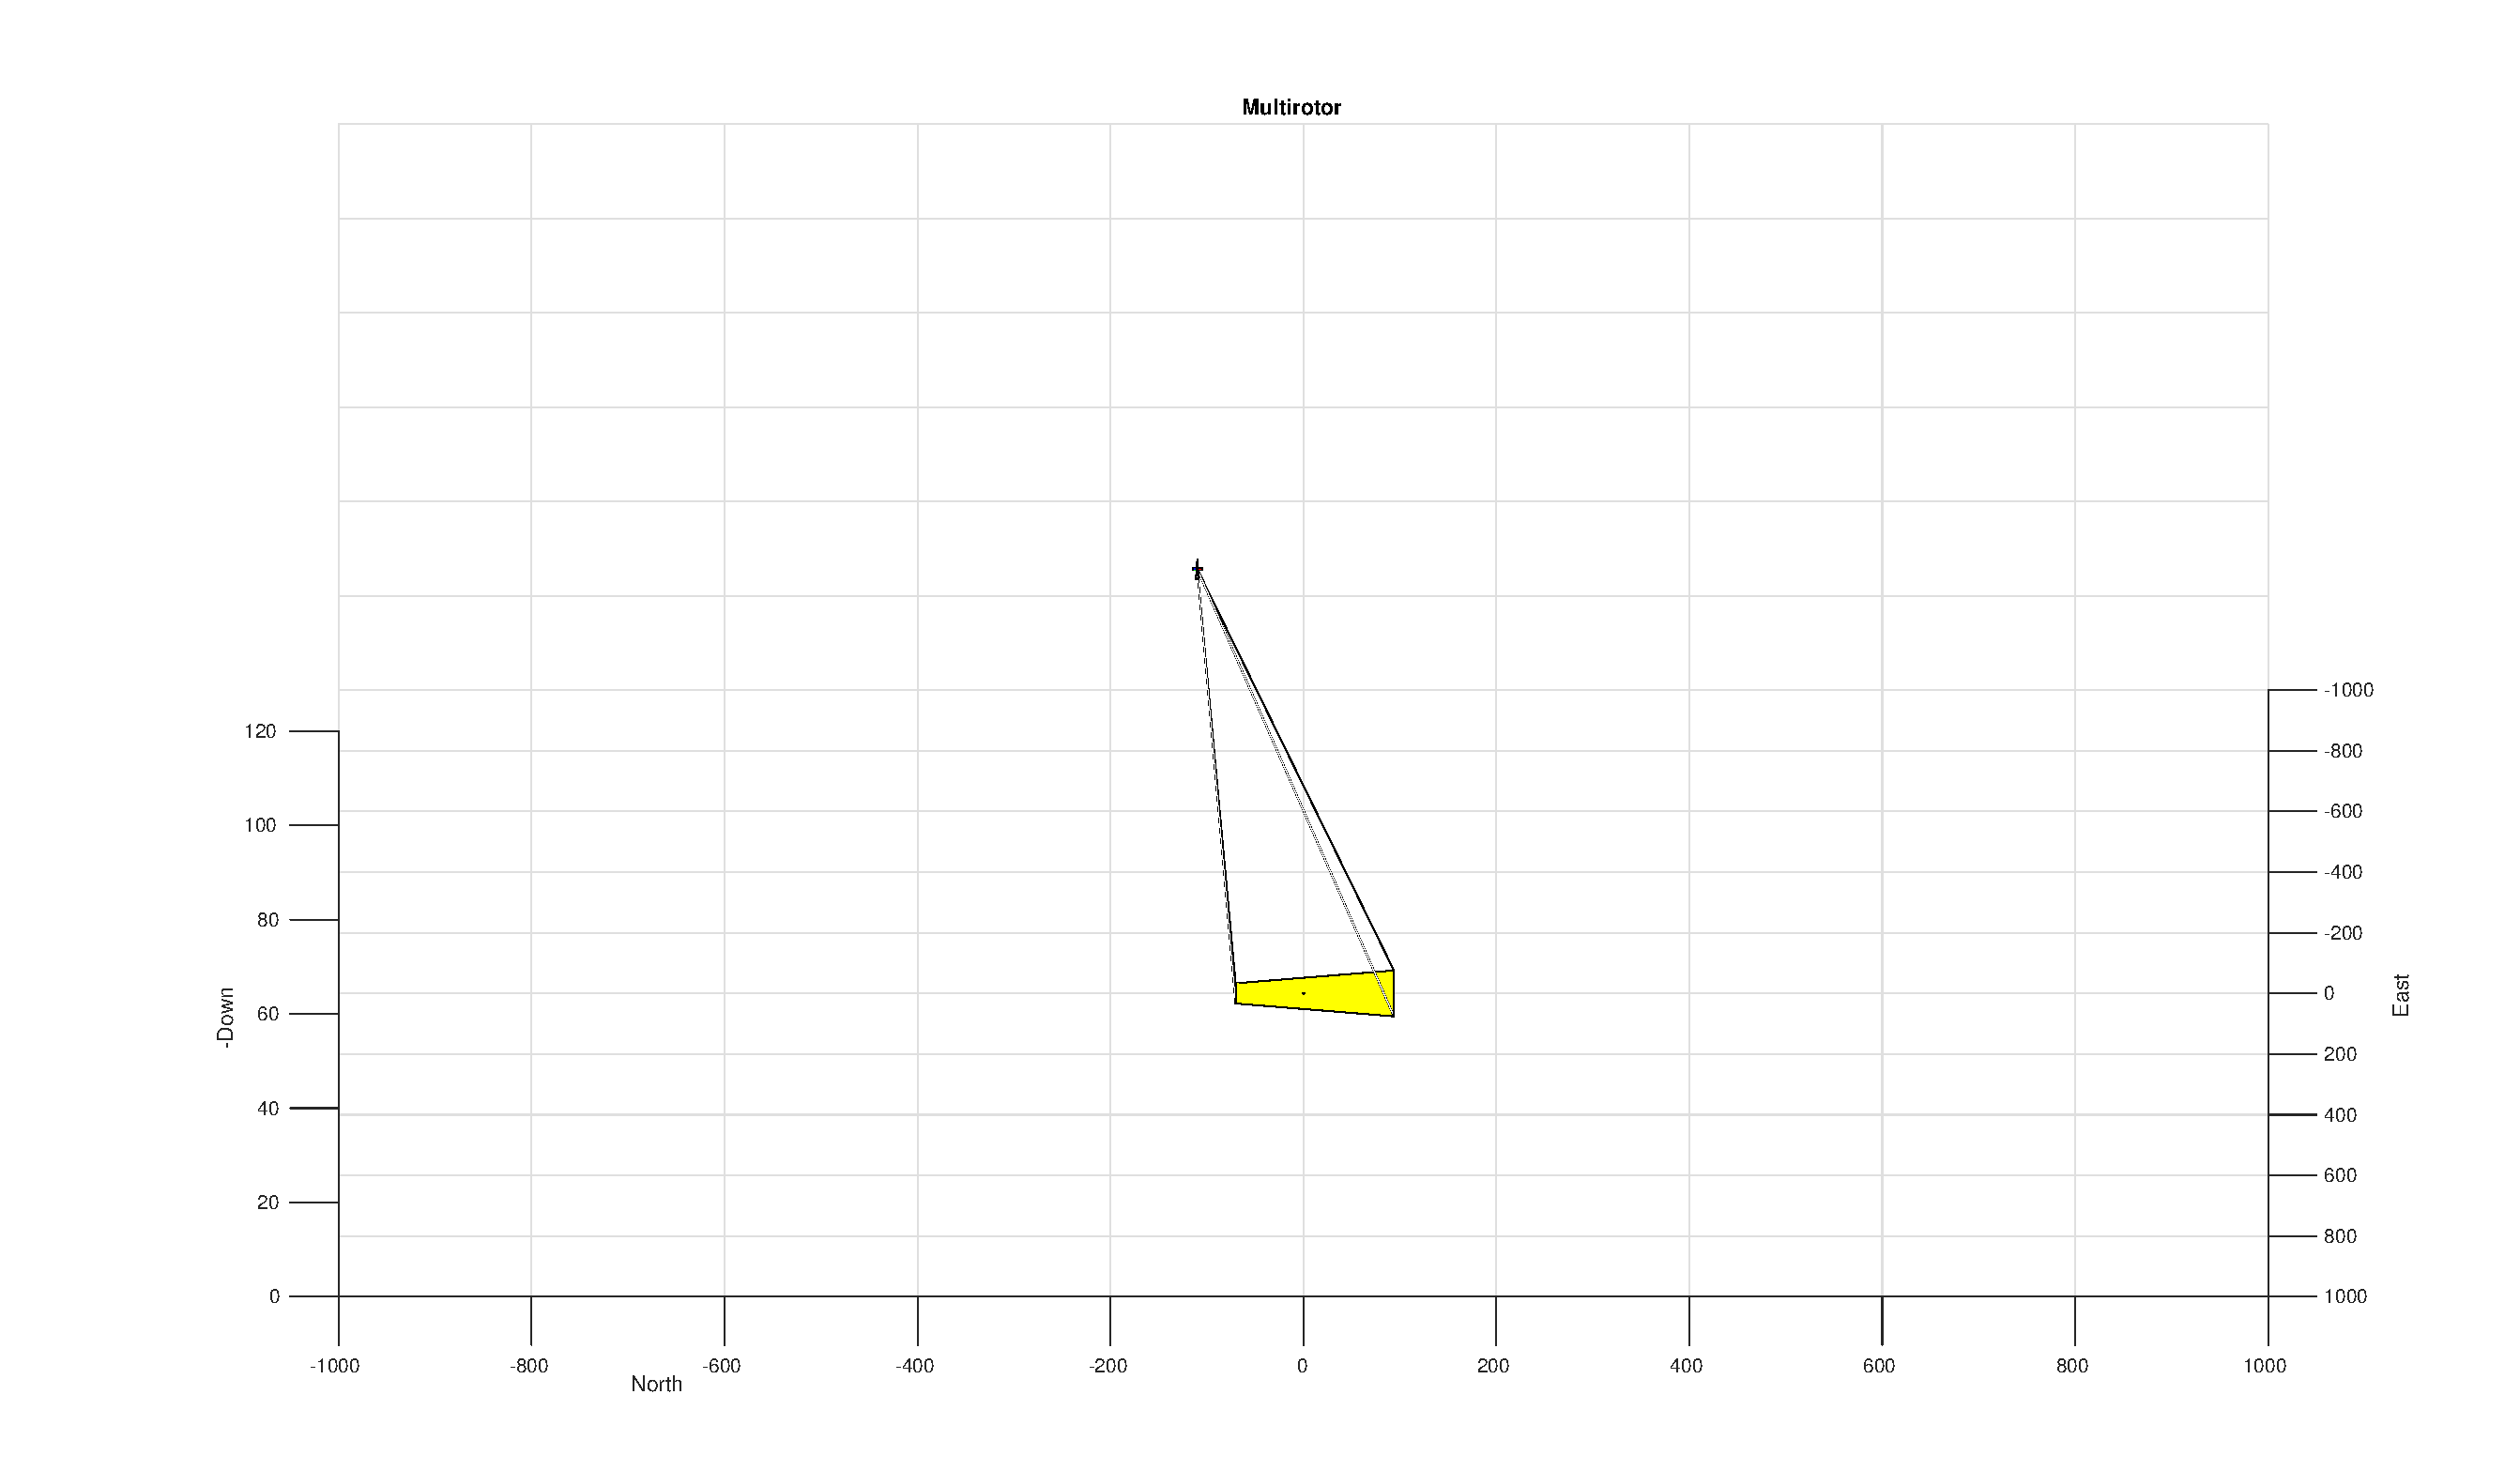
\includegraphics[width=\textwidth]{images/chapter4/image_UAV_5mps}
		\caption{when $t=0s$}
	\end{subfigure}
	\begin{subfigure}[t]{0.32\linewidth}
		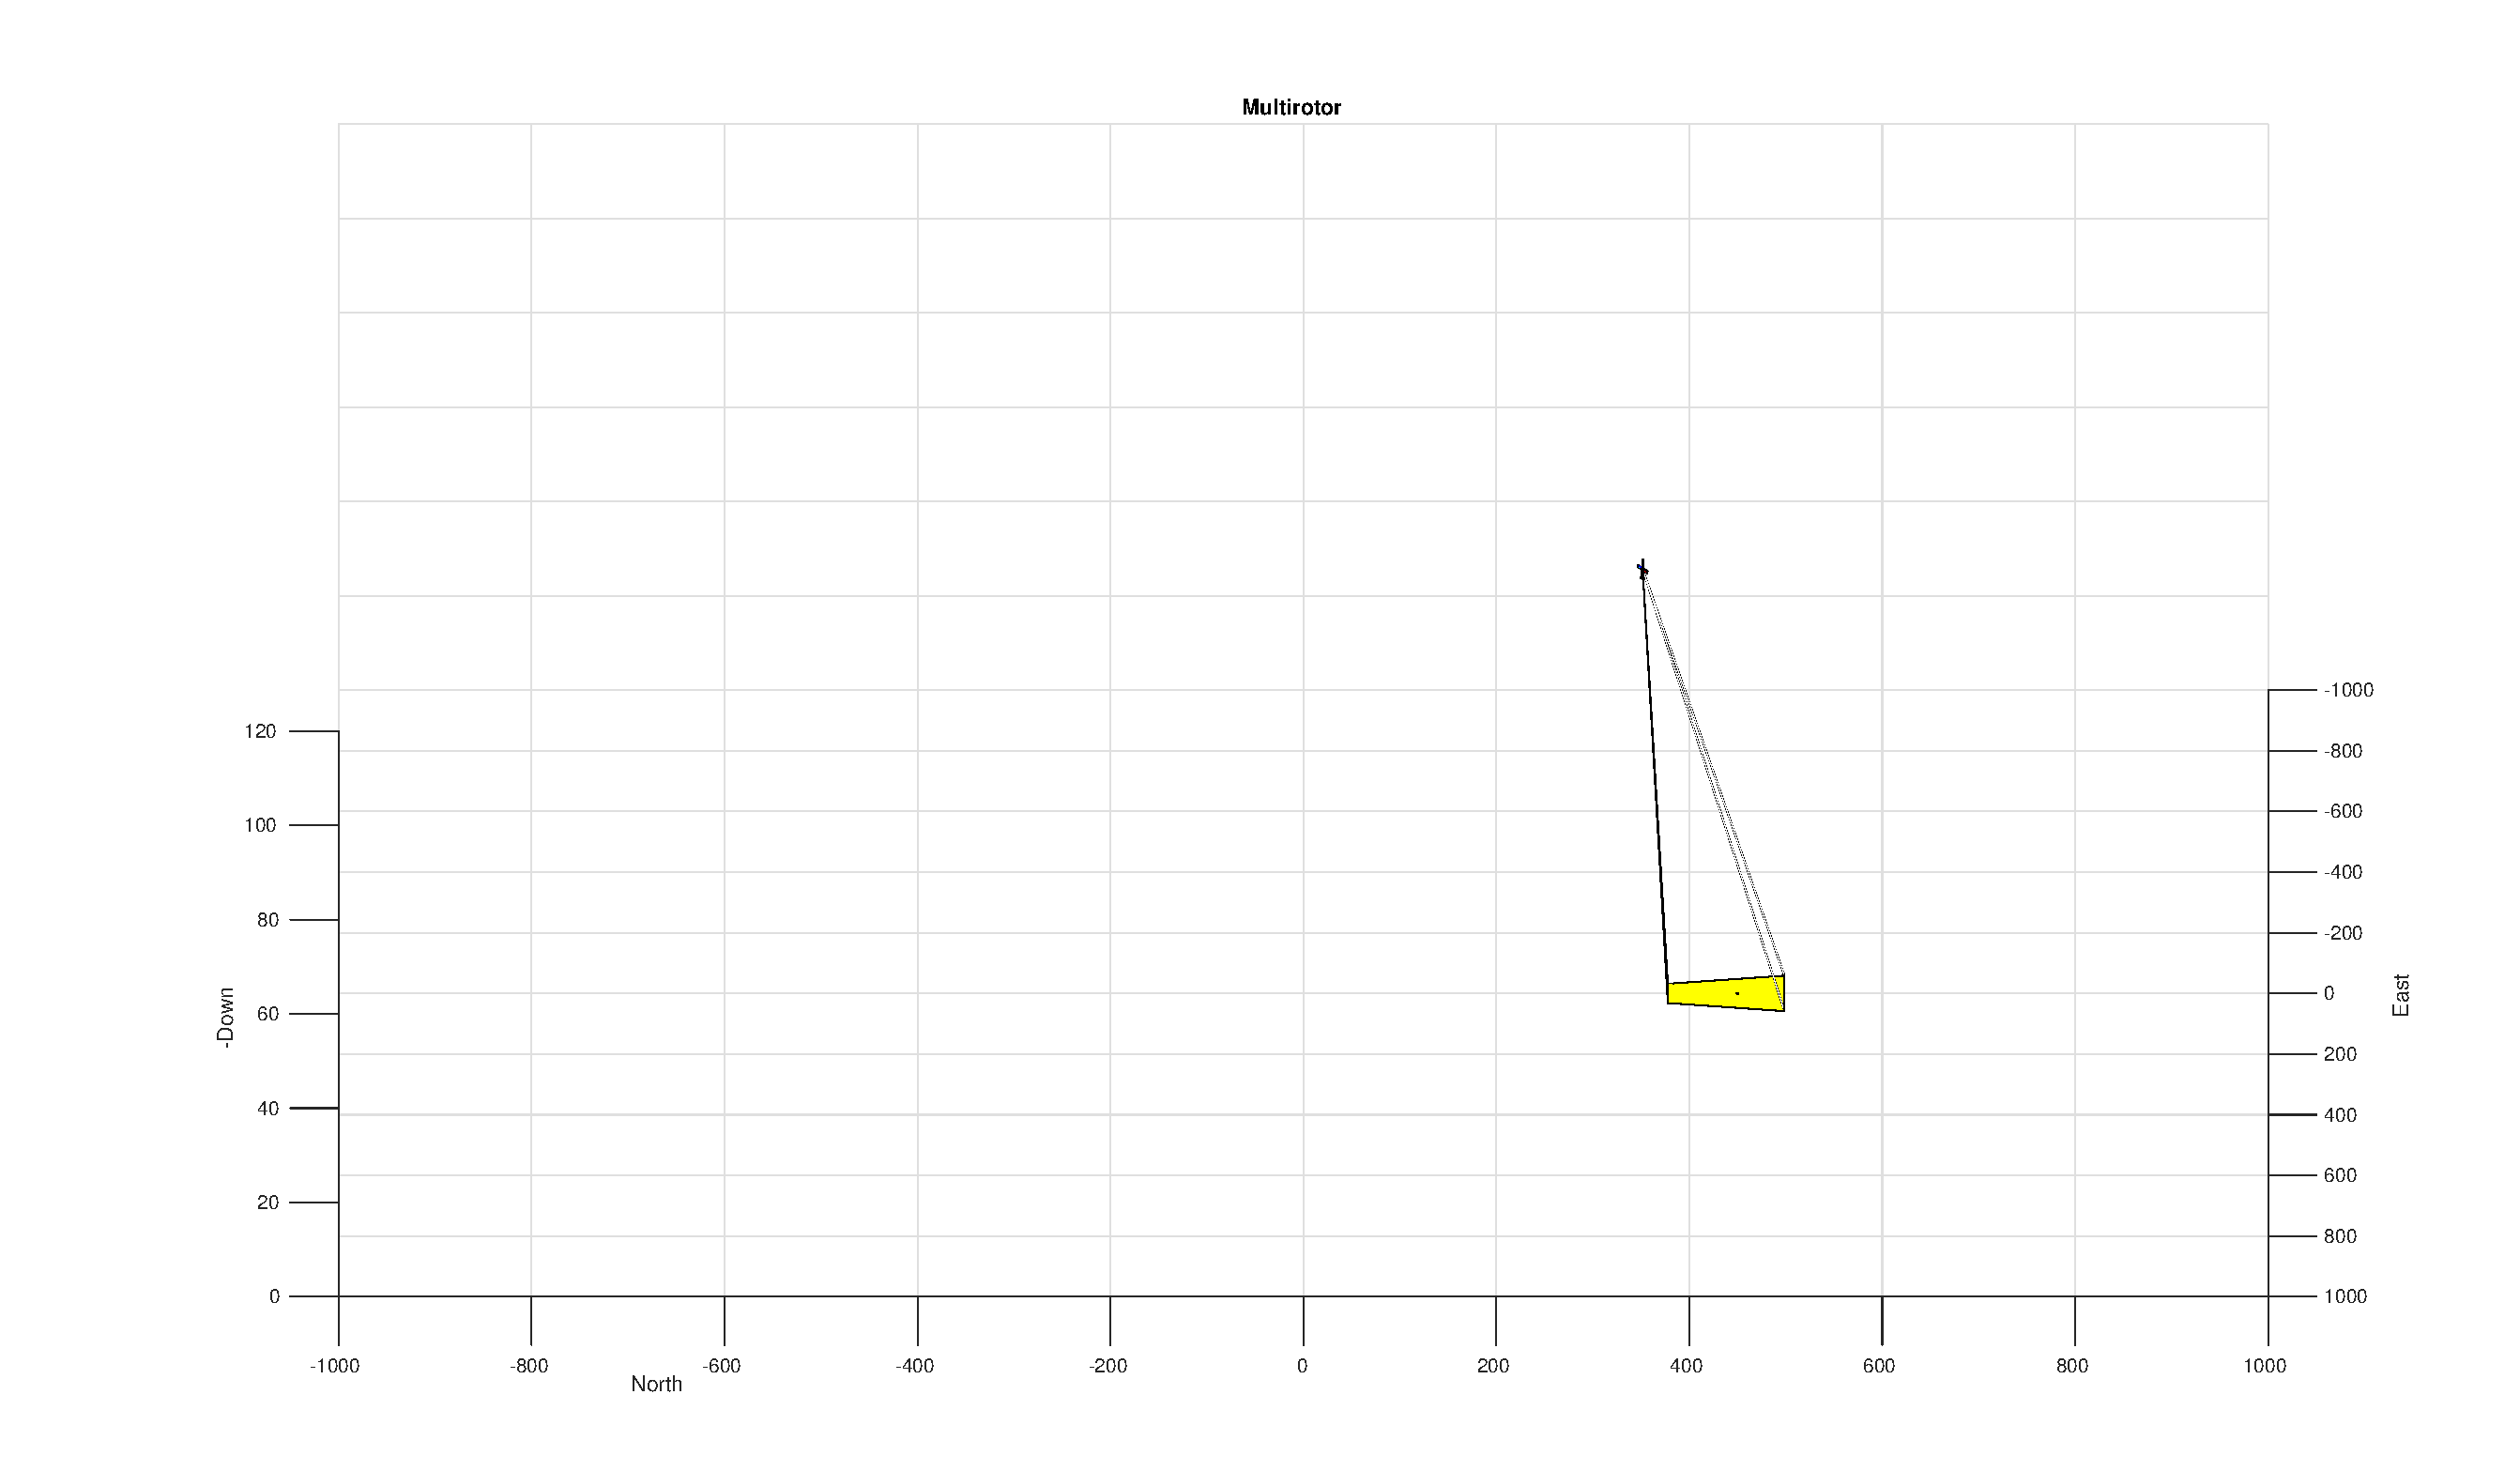
\includegraphics[width=\textwidth]{images/chapter4/image_UAV_5mps_90s}
		\caption{when $t=90s$}
	\end{subfigure}
	\begin{subfigure}[t]{0.32\linewidth}
		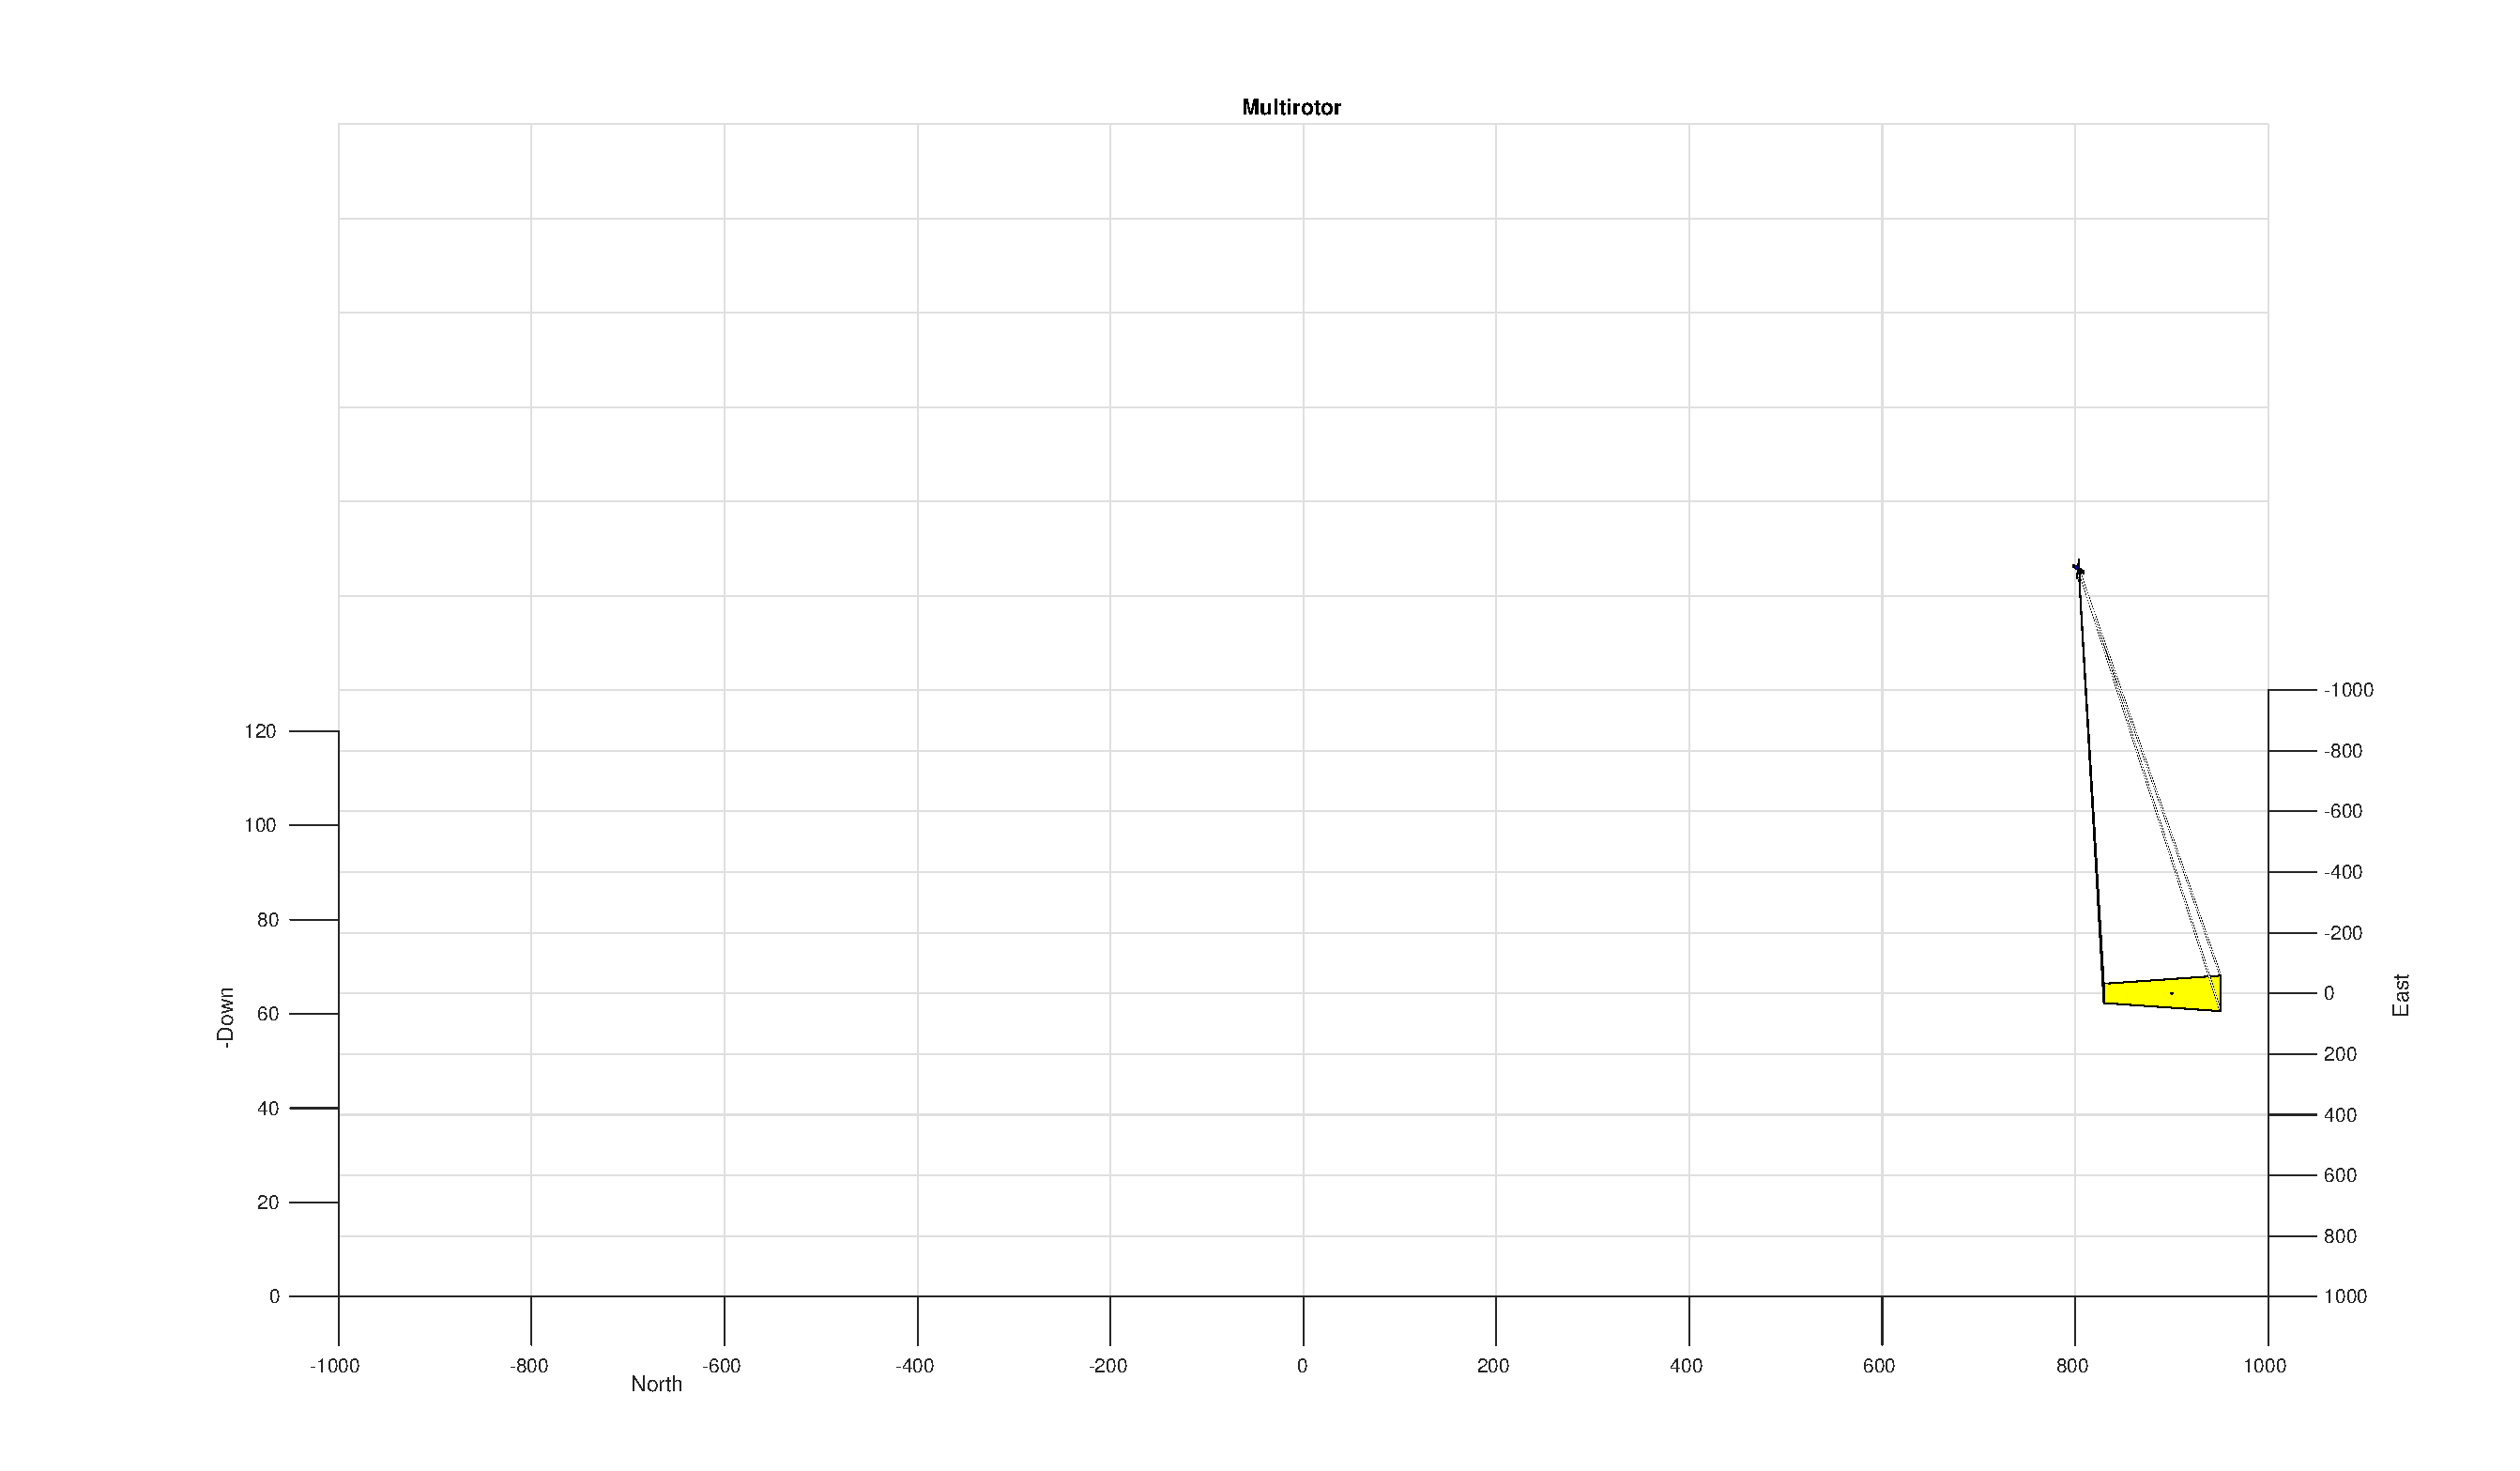
\includegraphics[width=\textwidth]{images/chapter4/image_UAV_5mps_180s}
		\caption{when $t=180s$}
	\end{subfigure}
	\begin{subfigure}[t]{0.32\linewidth}
		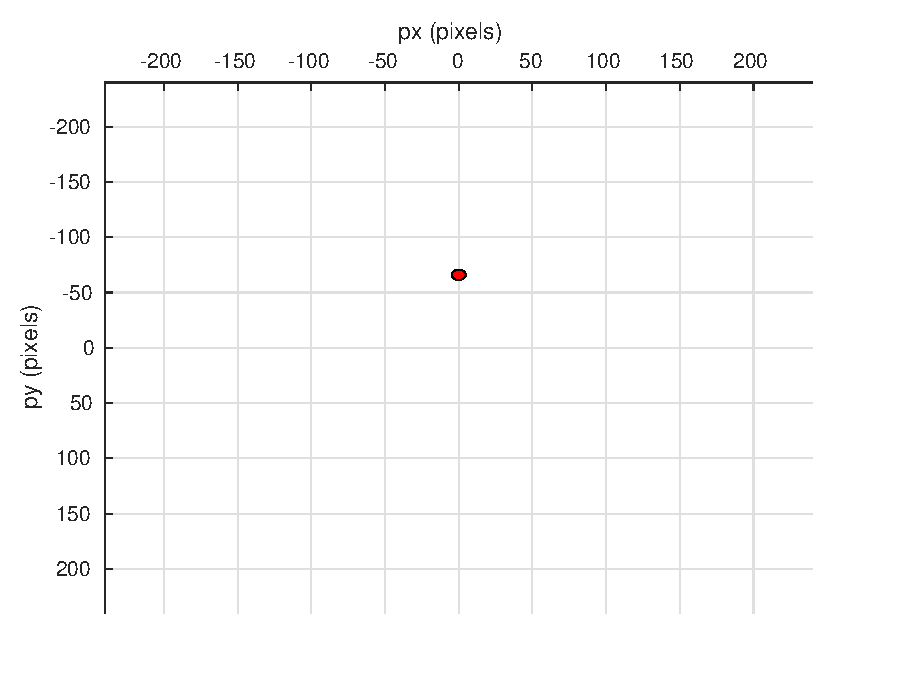
\includegraphics[width=\textwidth]{images/chapter4/image_camera_5mps}
		\caption{when $t=0s$}
	\end{subfigure}
	\begin{subfigure}[t]{0.32\linewidth}
		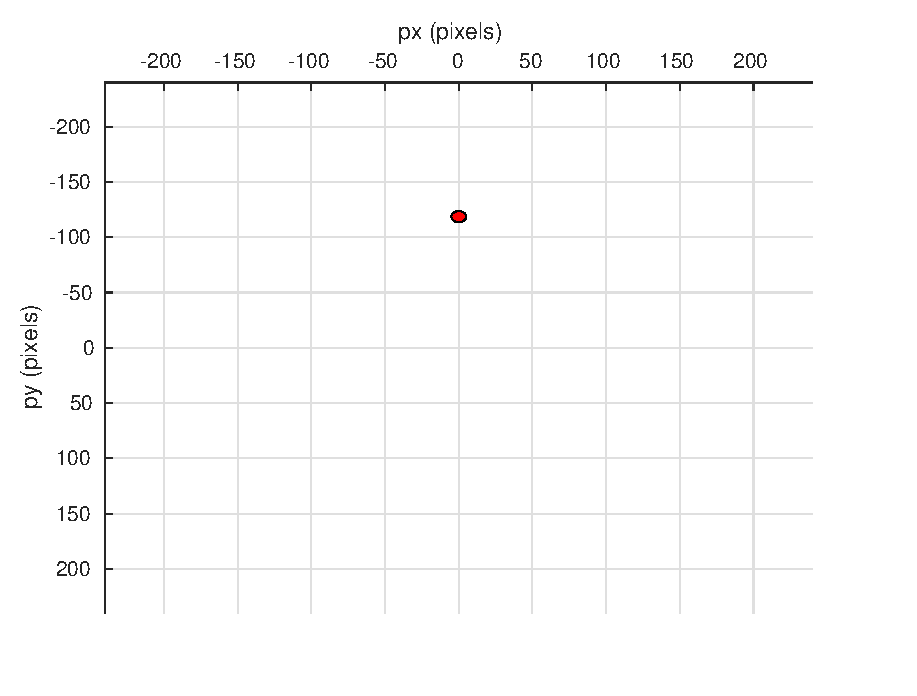
\includegraphics[width=\textwidth]{images/chapter4/image_camera_5mps_90s}
		\caption{when $t=90s$}
	\end{subfigure}
	\begin{subfigure}[t]{0.32\linewidth}
		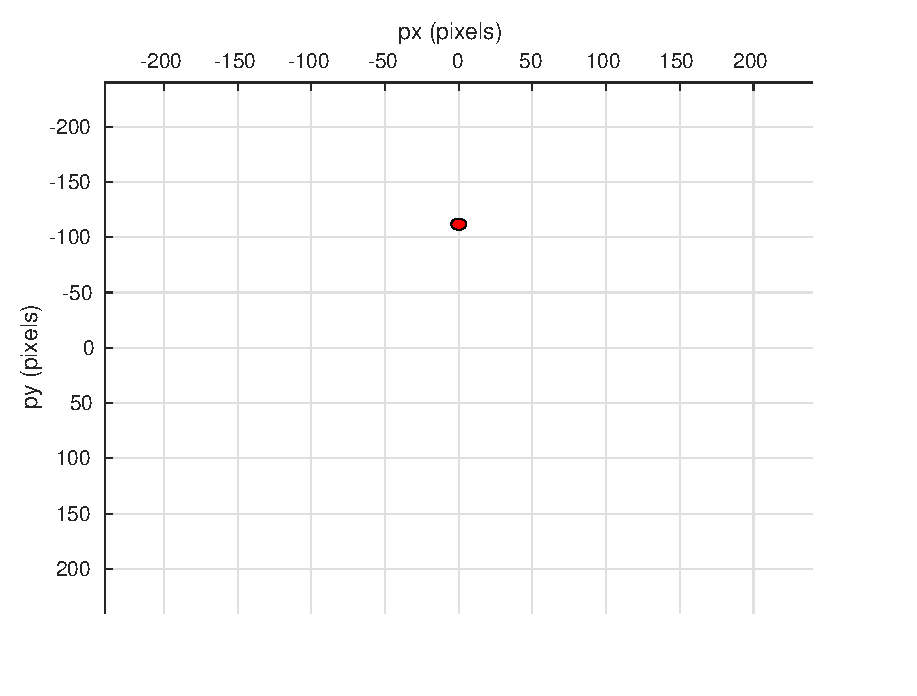
\includegraphics[width=\textwidth]{images/chapter4/image_camera_5mps_180s}
		\caption{when $t=180s$}
	\end{subfigure}	
	\begin{subfigure}[t]{0.8\linewidth}
		\centering
		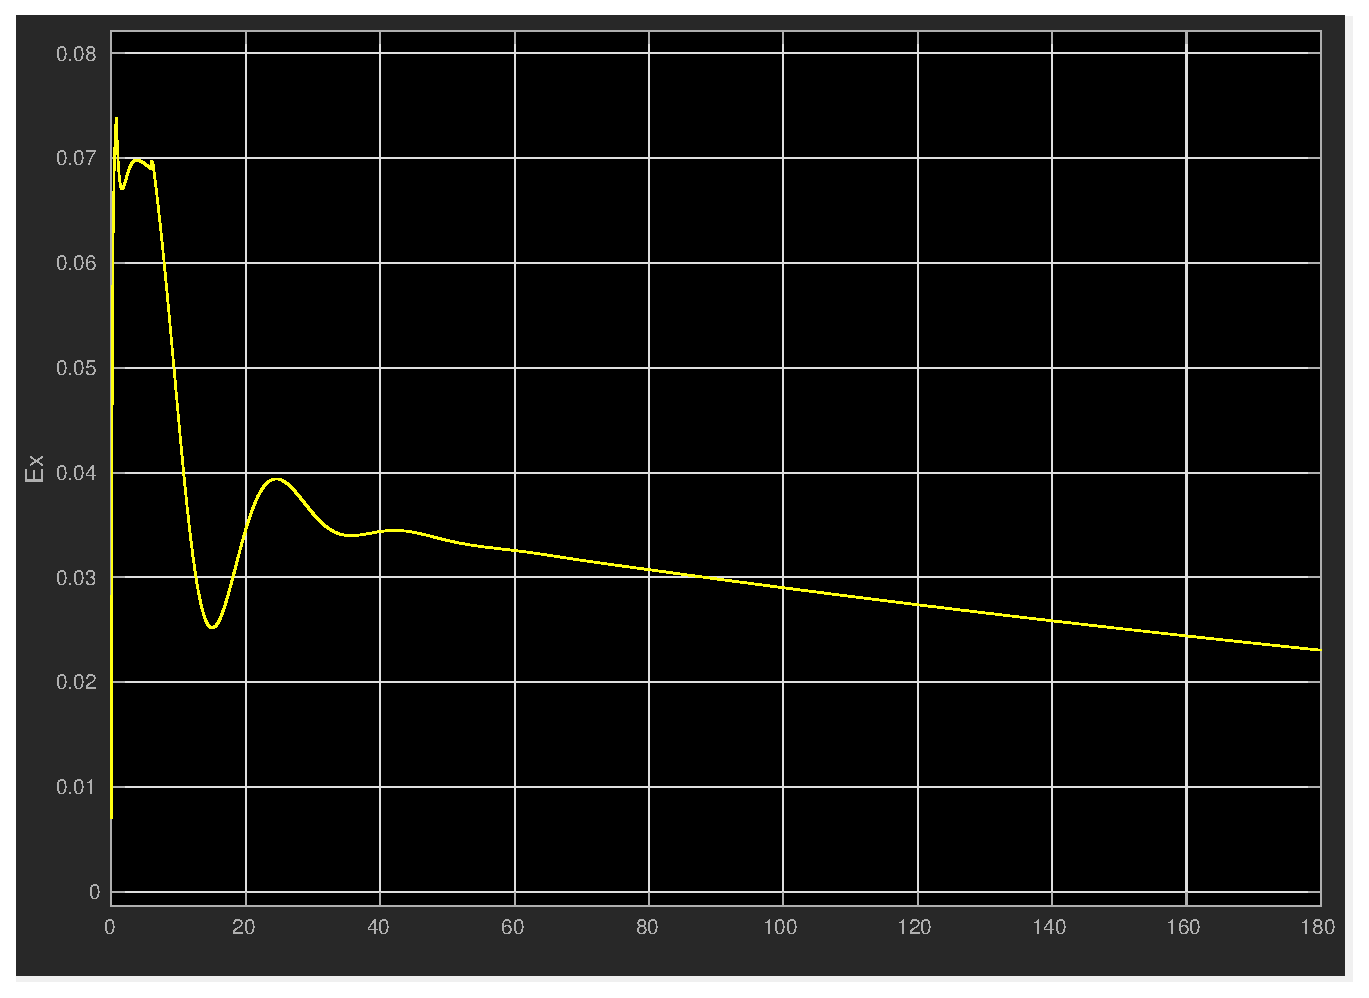
\includegraphics[width=0.5\textwidth]{images/chapter4/image_Ex_5mps}
		\caption{The horizontal error ($e_x$) between the normalized target pixel coordinates and the unit optical axis vector both in the vehicle-1 frame converges to zero. Note that the value is low-pass filtered.}
	\end{subfigure}	
	\caption{Simulation result for the backstepping control using the normalized target pixel coordinates. The ground target is moving at the speed of $5m/s$. The initial UAV and target positions are [-110, 0, -90] and [0, 0, 0] respectively. Tuning parameters are set to $k=0.12$, $k_1=1$, $k_2=1$, $k_3=1$, and $\Gamma=0.01*I_3$ (identity matrix). In this case, the target is not placed at the center of image because the horizontal error is computed in the vehicle-1 frame meaning that the pitch of multirotor is not compensated.}
	\label{image_5mps}
\end{figure}

\begin{figure}[htbp]
	\centering
	\begin{subfigure}[t]{0.32\linewidth}
		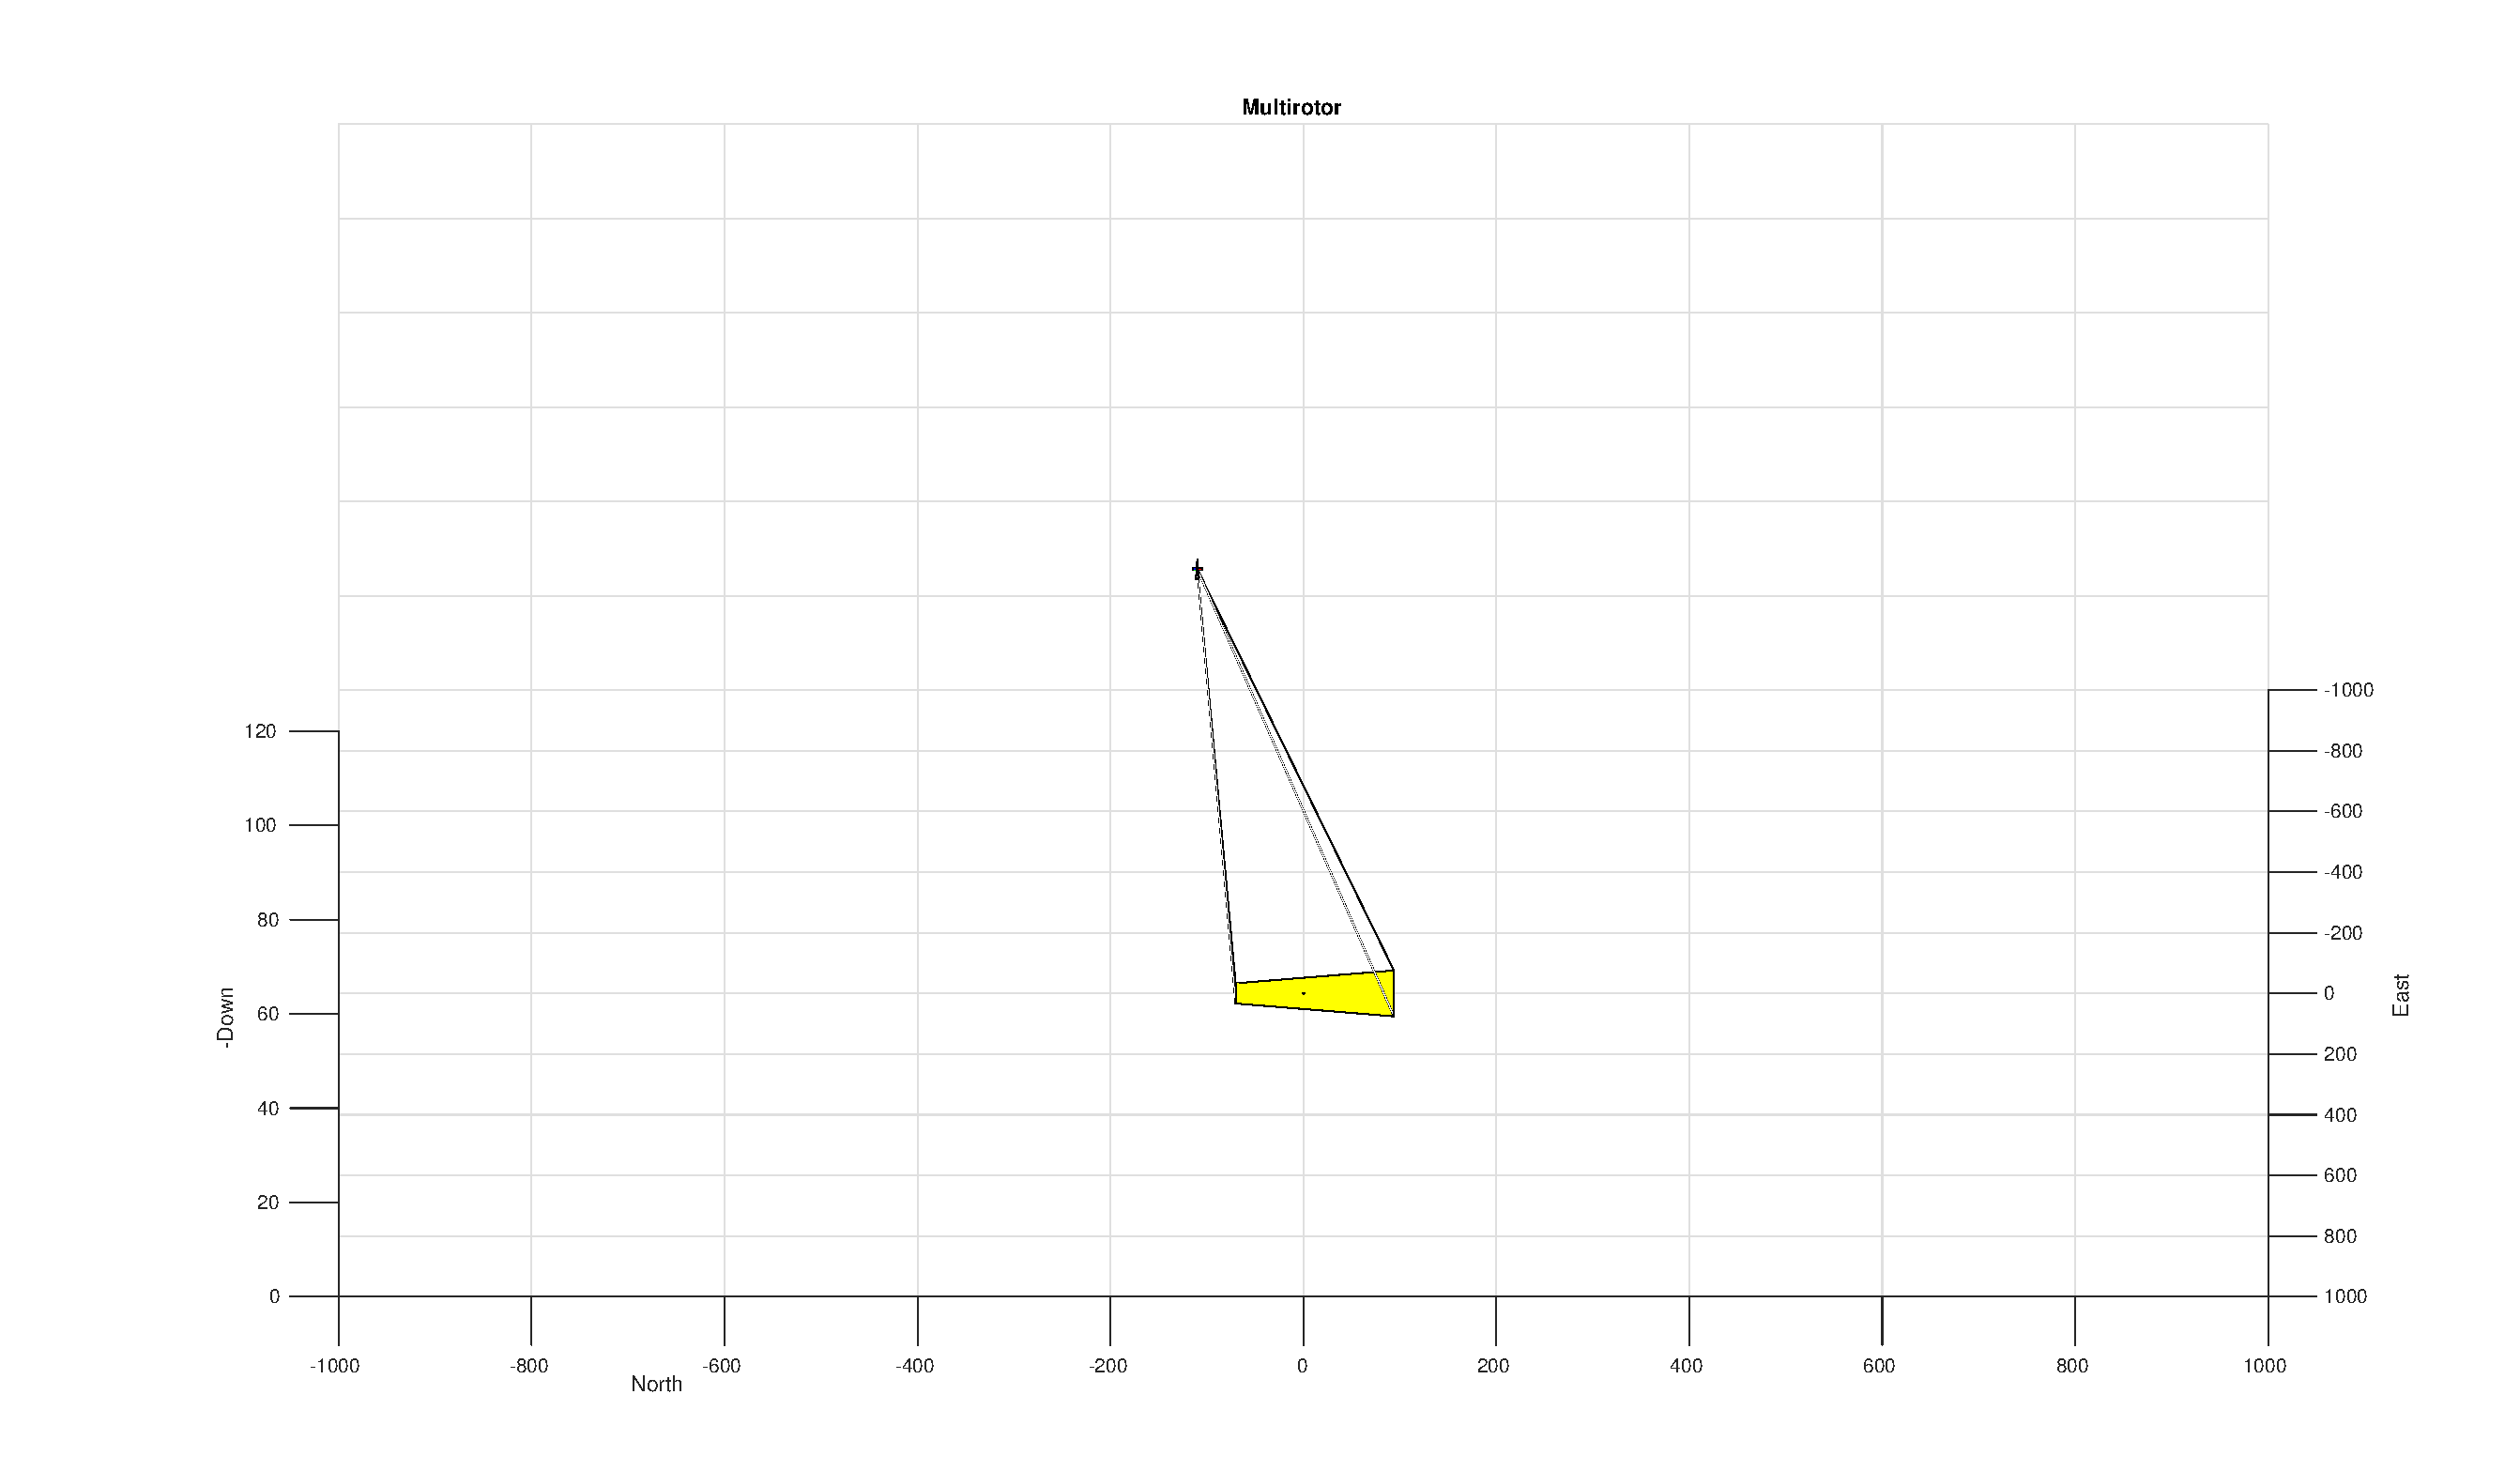
\includegraphics[width=\textwidth]{images/chapter4/image_UAV_-5mps}
		\caption{when $t=0s$}
	\end{subfigure}
	\begin{subfigure}[t]{0.32\linewidth}
		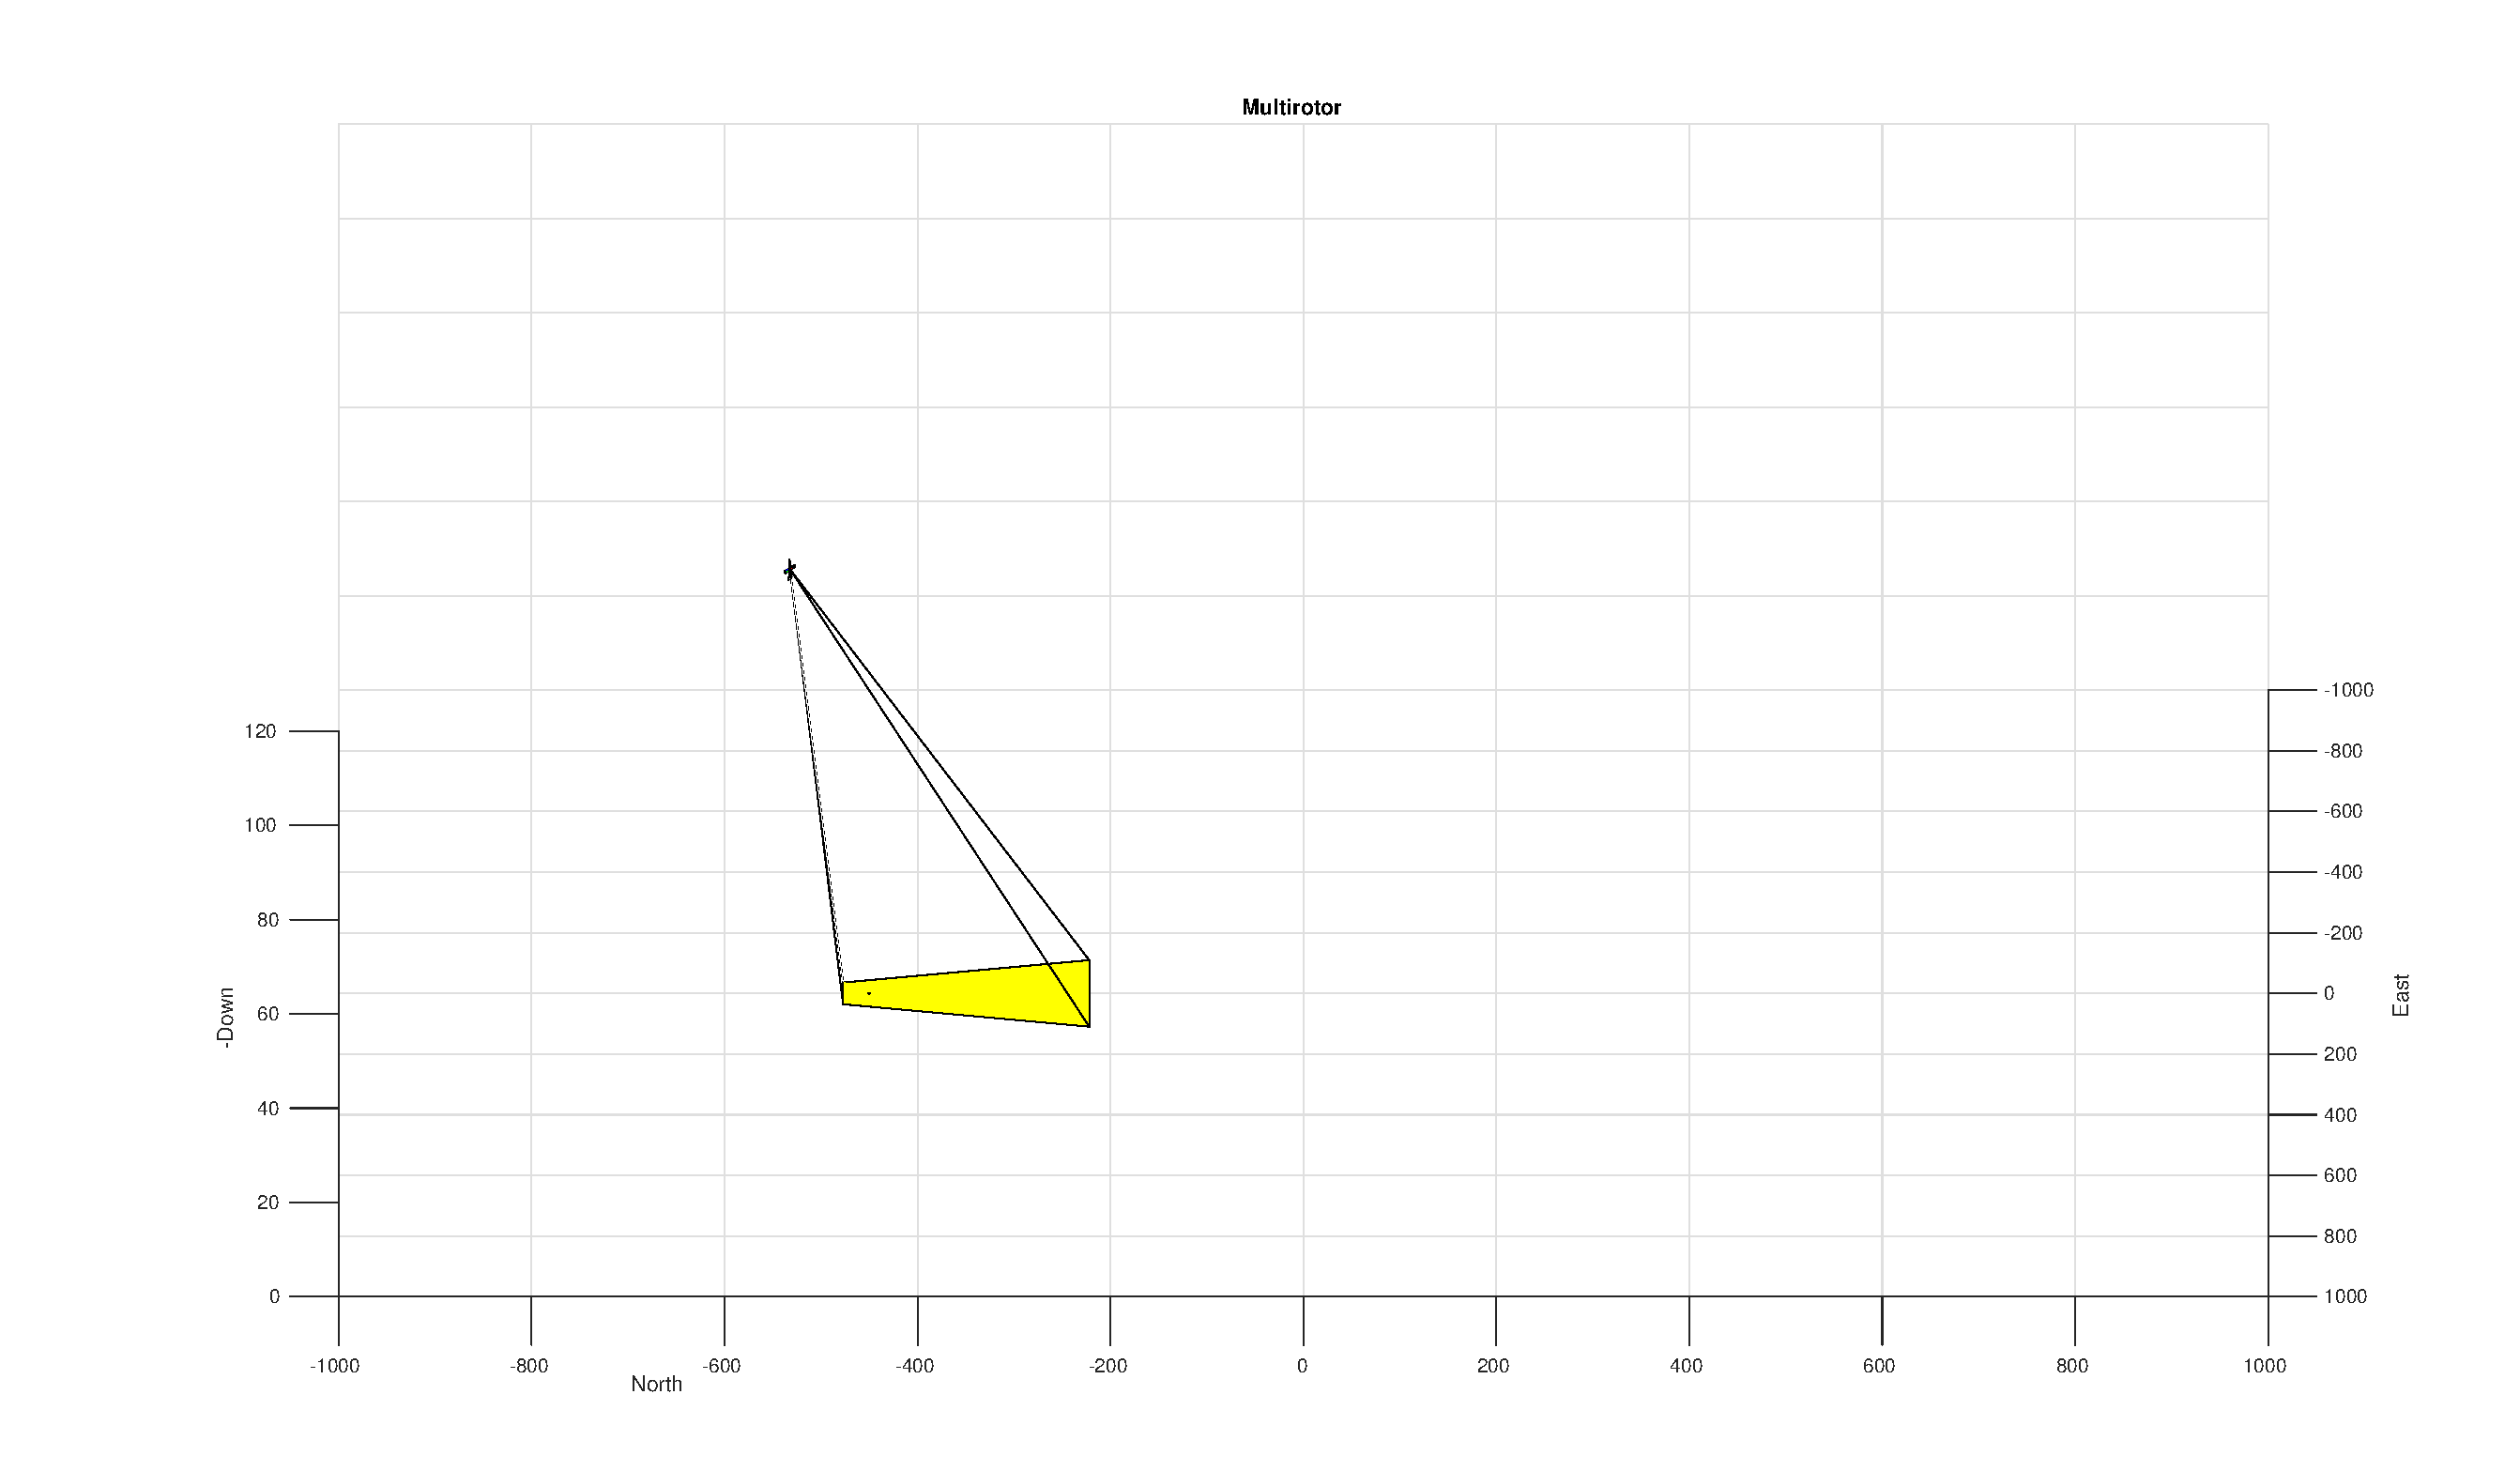
\includegraphics[width=\textwidth]{images/chapter4/image_UAV_-5mps_90s}
		\caption{when $t=90s$}
	\end{subfigure}
	\begin{subfigure}[t]{0.32\linewidth}
		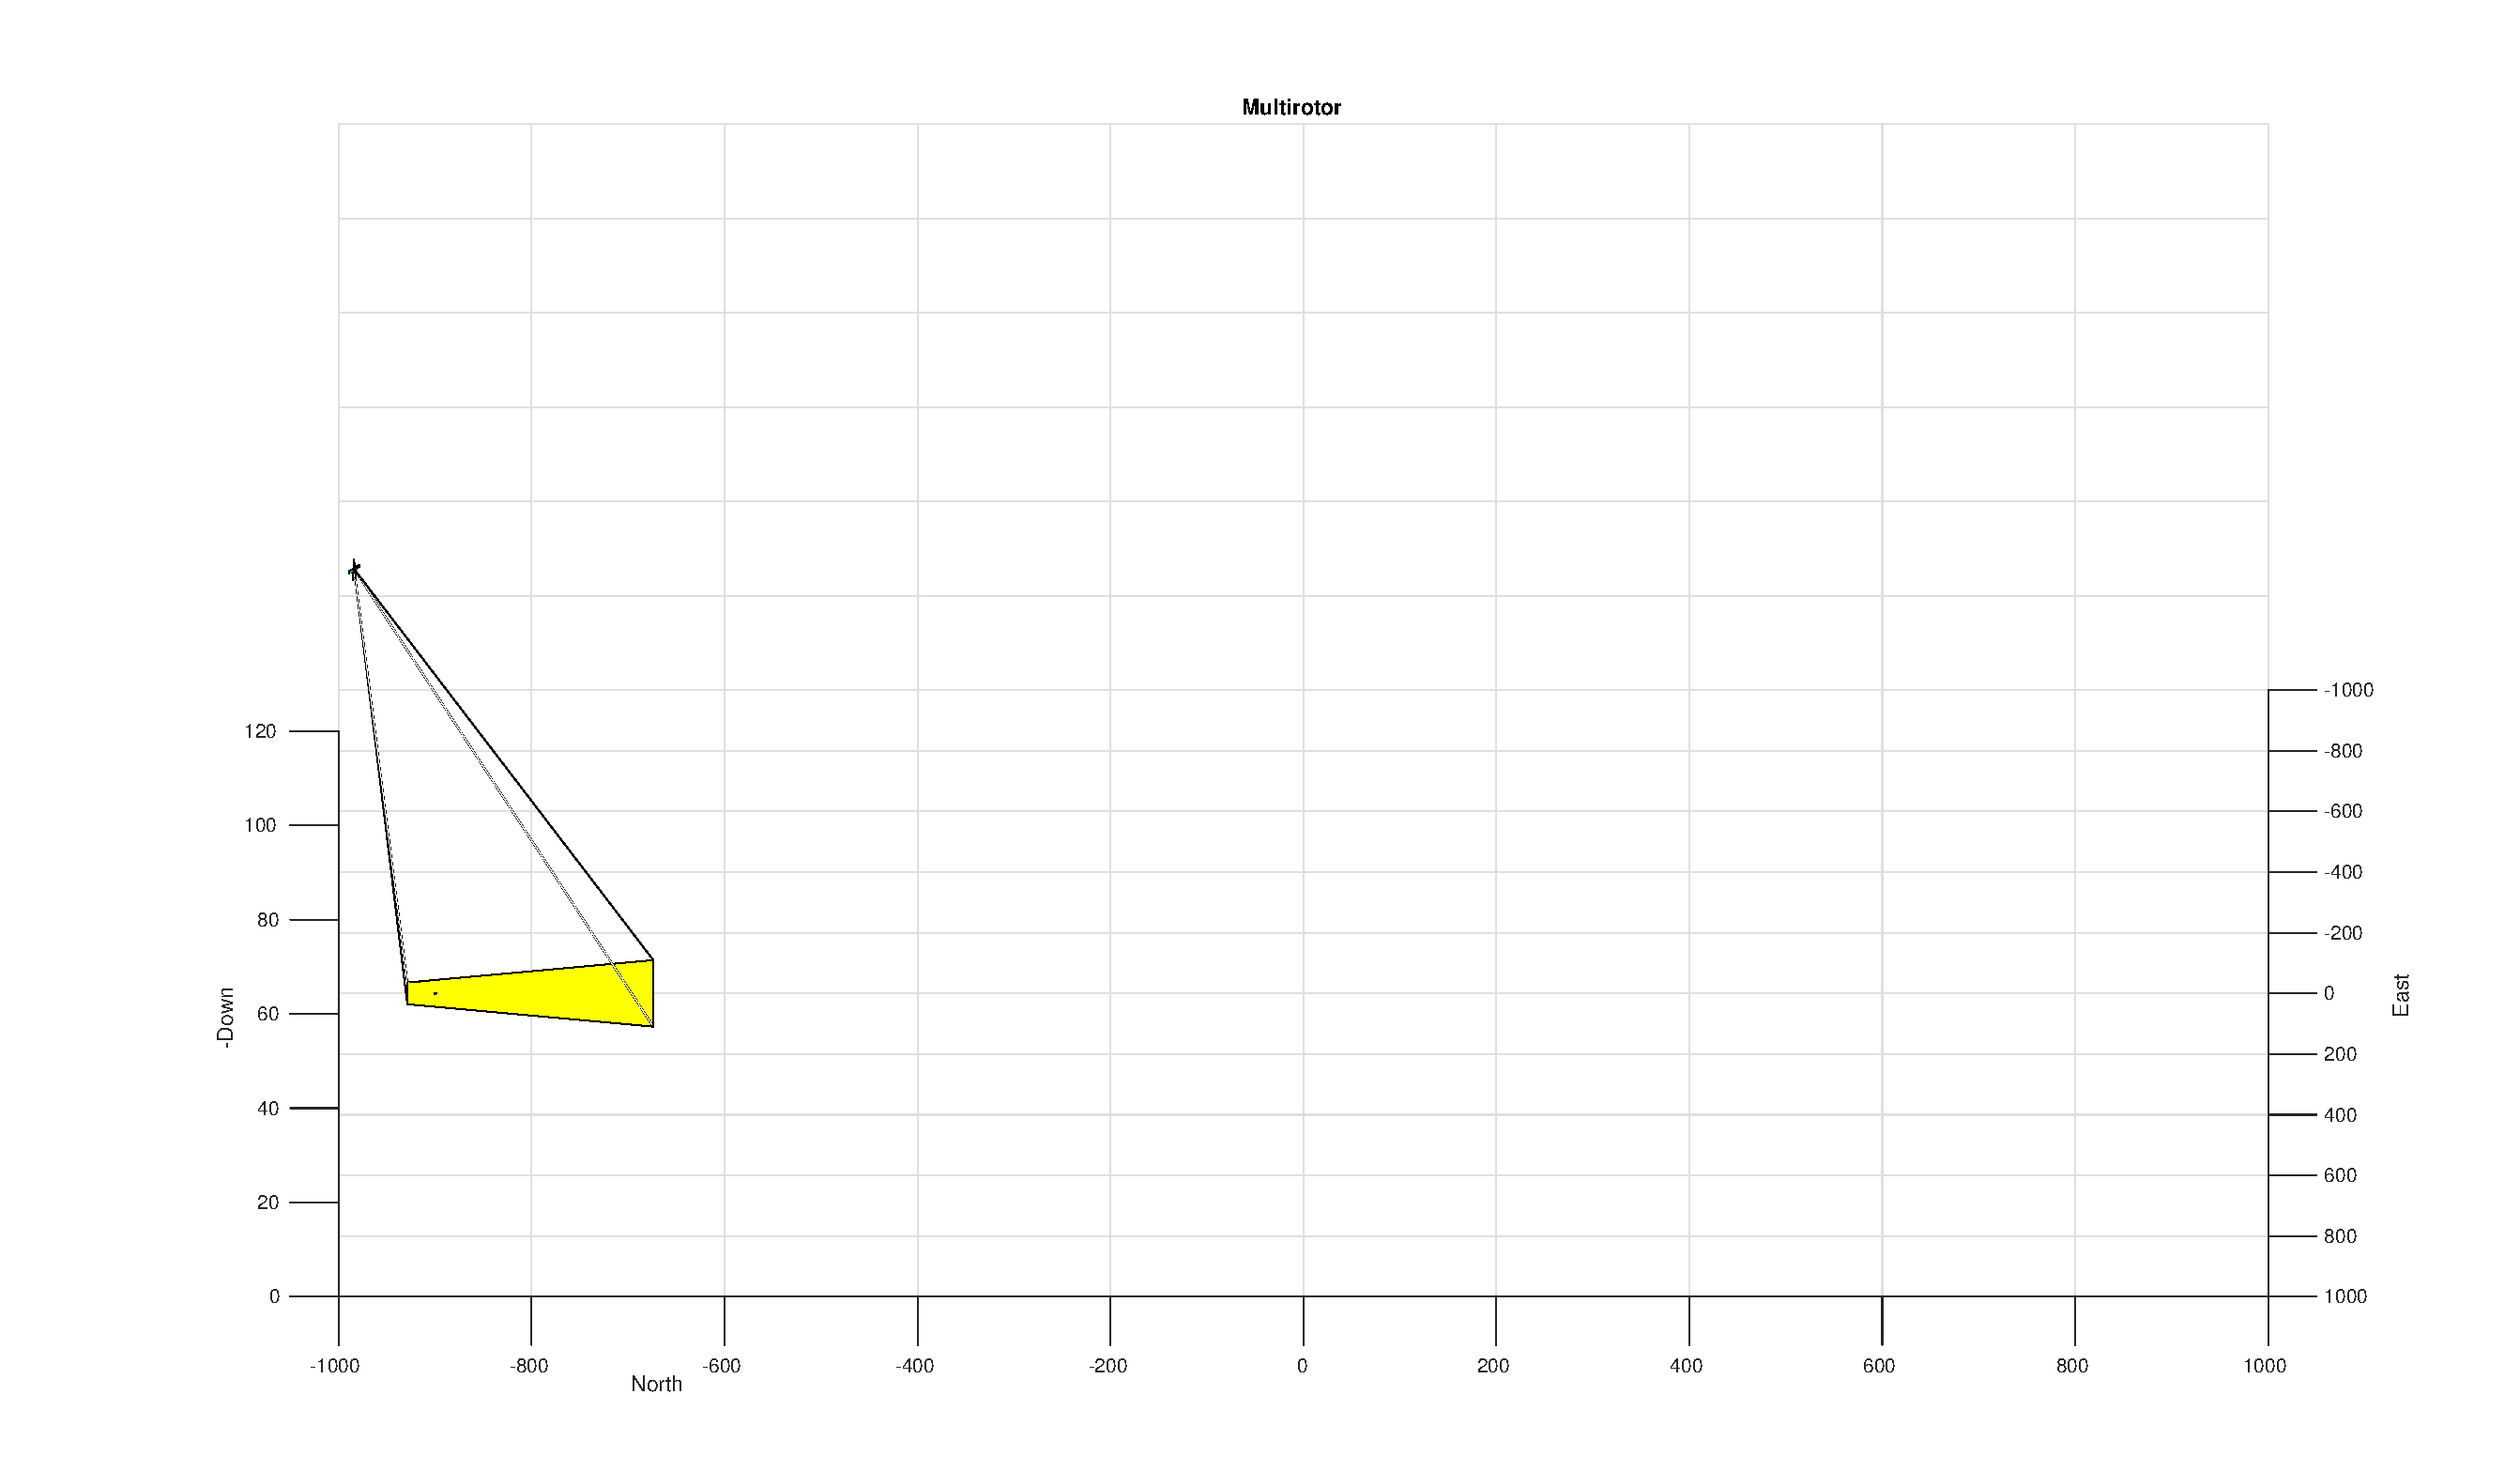
\includegraphics[width=\textwidth]{images/chapter4/image_UAV_-5mps_180s}
		\caption{when $t=180s$}
	\end{subfigure}
	\begin{subfigure}[t]{0.32\linewidth}
		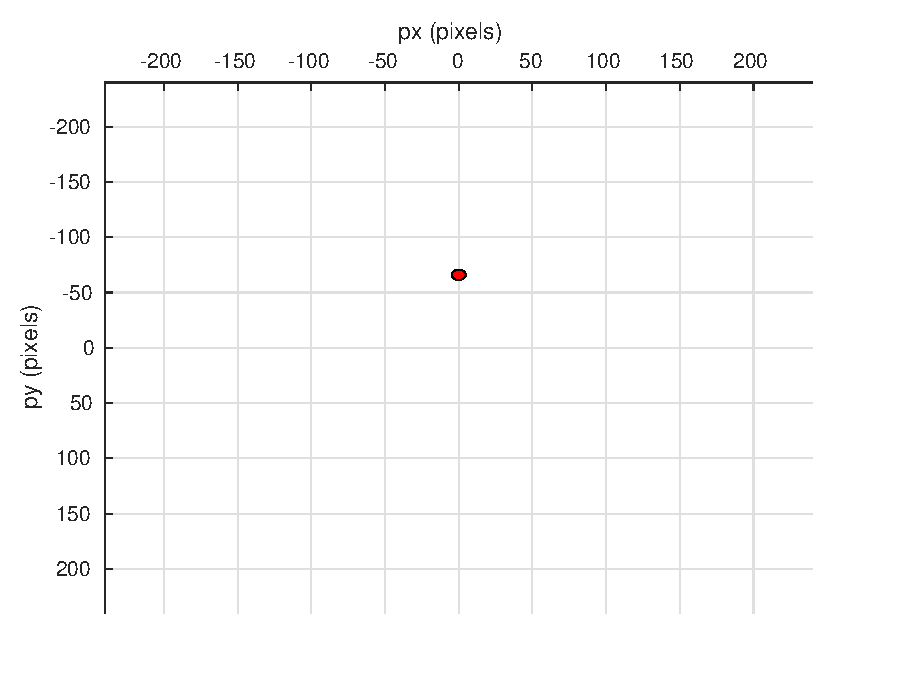
\includegraphics[width=\textwidth]{images/chapter4/image_camera_-5mps}
		\caption{when $t=0s$}
	\end{subfigure}
	\begin{subfigure}[t]{0.32\linewidth}
		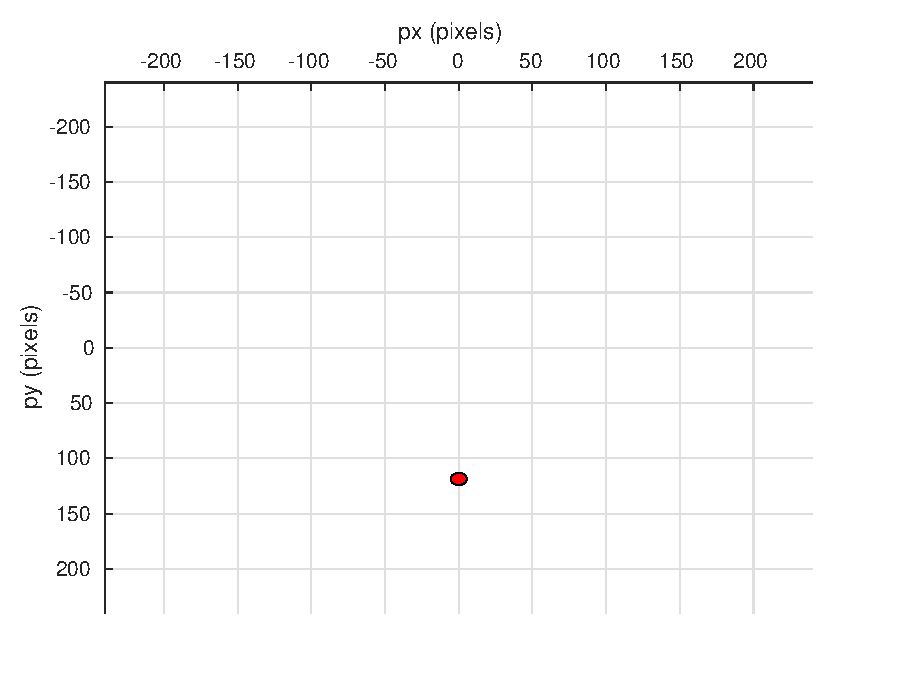
\includegraphics[width=\textwidth]{images/chapter4/image_camera_-5mps_90s}
		\caption{when $t=90s$}
	\end{subfigure}
	\begin{subfigure}[t]{0.32\linewidth}
		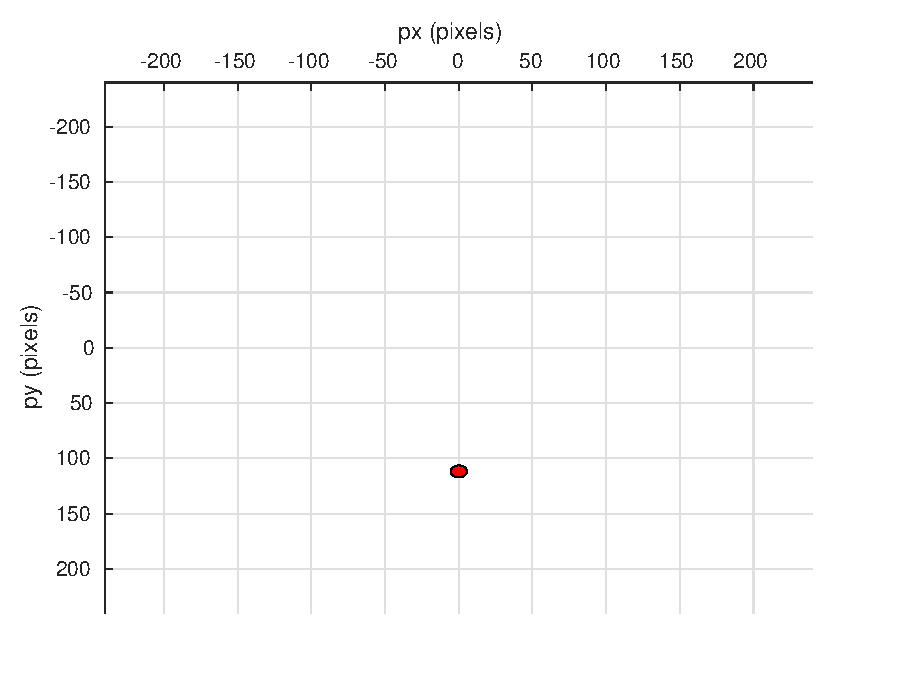
\includegraphics[width=\textwidth]{images/chapter4/image_camera_-5mps_180s}
		\caption{when $t=180s$}
	\end{subfigure}	
	\begin{subfigure}[t]{0.8\linewidth}
		\centering
		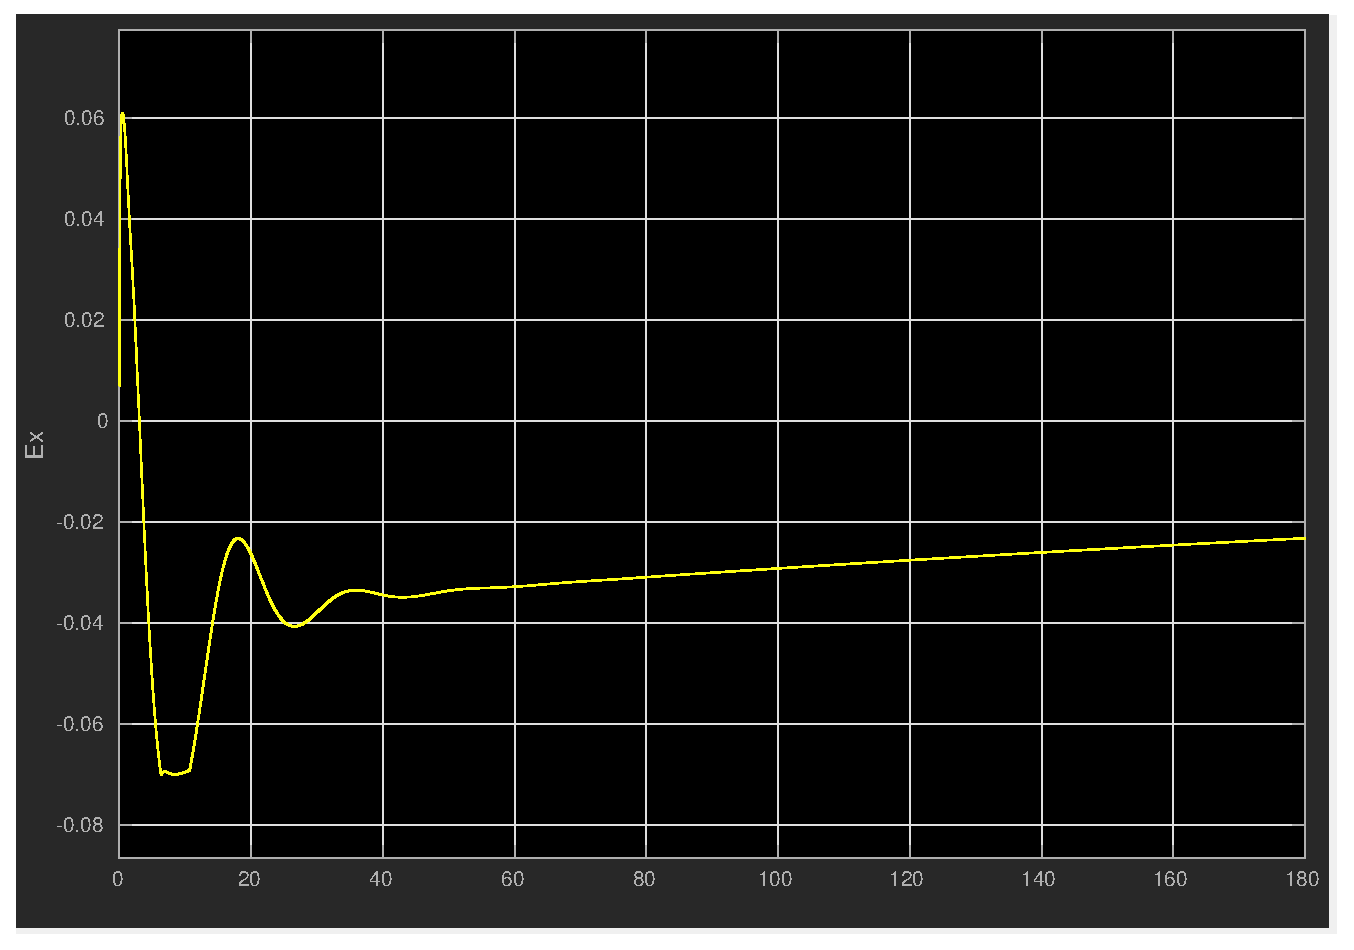
\includegraphics[width=0.5\textwidth]{images/chapter4/image_Ex_-5mps}
		\caption{The horizontal error ($e_x$) between the normalized target pixel coordinates and the unit optical axis vector both in the vehicle-1 frame converges to zero. Note that the value is low-pass filtered.}
	\end{subfigure}	
	\caption{Simulation result for the backstepping control using the normalized target pixel coordinates. The ground target is moving at the speed of $-5m/s$. The initial UAV and target positions are [-110, 0, -90] and [0, 0, 0] respectively. Tuning parameters are set to $k=0.12$, $k_1=1$, $k_2=1$, $k_3=1$, and $\Gamma=0.01*I_3$ (identity matrix). In this case, the target is not placed at the center of image because the horizontal error is computed in the vehicle-1 frame meaning that the pitch of multirotor is not compensated.}
	\label{image_-5mps}
\end{figure}